\documentclass[12pt, a4paper, reqno]{article}
\usepackage{preamble}

\title{\bf Билеты к устному экзамену \\ Введение в математический анализ}
\date{}
\author{by \href{https://github.com/KetchuppOfficial}{KetchuppOfficial}}

\begin{document}

\maketitle

\newpage
\tableofcontents
\newpage

\section{БИЛЕТ 1}

\subsection{Действительные числа}

    \textbf{Определение}: Сечением $\alpha$ множества $\mathbb{Q}$ называется такое
    разбиение $\mathbb{Q}$ на два непустых множества $A$ и $A'$ ($A \cap A' = \emptyset$,
    $A \cup A' = \mathbb{Q}$), что $\forall x \in A$, $\forall x' \in A'$ $\hookrightarrow$
    $x < x'$; множество $A$ называется нижним классом сечения, множество $A'$ -- верхним
    классом сечения; применяется обозначение $\alpha = A|A'$.

    Существуют сечения трёх типов:
    \begin{enumerate}
        \item В $A$ есть наибольший элемент, в $A'$ нет наименьшего элемент;
        \item В $A$ нет наибольшего элемента, в $A'$ есть наименьший элемент;
        \item В $A$ нет наибольшего элемента, в $A'$ нет наименьшего элемента.
    \end{enumerate}

    Сечений 4-го типа, когда в нижнем классе есть наибольший элемент, а в верхнем -- наименьший, нет.

    $\square$ Пусть $\exists r_1 \in A$, $\exists r_2 \in A'$ -- соответственно наибольший и
    наименьший элементы в этих классах. Рассмотрим $r_0 = \dfrac{r_1 + r_2}{2} \in \mathbb{Q}$. Так
    как $r_0 > r_1$, то $r_0 \not\in A$; так как $r_0 < r_2$, то $r_0 \not\in A'$
    $\implies r_0 \not\in \mathbb{Q}$ -- противоречие. $\blacksquare$

    \textbf{Определение}: иррациональным числом называется сечение III типа.

    \textbf{Определение}: действительным числом называется любое сечение II или III типа (в нижнем
    классе нет наибольшего элемента).

    \textbf{Определение}: два действительных числа $\alpha = A|A'$ и $\beta = B|B'$ называют равными,
    если $A = B$.

    \textbf{Определение}: рассмотрим два действительных числа $\alpha = A|A'$ и $\beta = B|B'$;
    говорят, что $\alpha < \beta$, если $A \subset B$, $\alpha > \beta$, если $A \supset B$
    (включения считаются строгими).

    \textbf{Теорема}: если действительные числа $\alpha \neq \beta$, то либо $\alpha < \beta$, либо
    $\alpha > \beta$.

    $\square$ Пусть $\alpha = A|A'$ и $\beta = B|B'$; $\alpha \neq \beta \implies A \neq B$.
    Нужно доказать, что либо $A \subset B$, либо $A \supset B$. Если не выполнено $A \subset B$, то
    $\exists r_1 \in \mathbb{Q}: r_1 \in A, r_1 \not\in B$. Если не выполнено $A \supset B$, то
    $\exists r_2 \in \mathbb{Q}: r_2 \in B, r_2 \not\in A$.
    \begin{equation*}
        r_1 \not\in B \implies r_1 \in B'
    \end{equation*}
    \begin{equation*}
        r_2 \not\in A \implies r_2 \in A'
    \end{equation*}
    \begin{equation*}
        r_1 \in A,\ r_2 \in A' \implies r_1 < r_2
    \end{equation*}
    \begin{equation*}
        r_1 \in B',\ r_2 \in B \implies r_1 > r_2
    \end{equation*}
    Получено противоречие. $\blacksquare$

    \textbf{Теорема (плотность рациональных чисел в $\mathbb{R}$)}: $\forall \alpha, \beta \in
    \mathbb{R}, \alpha > \beta \hookrightarrow \exists r \in \mathbb{Q}: \alpha > r > \beta$.

    $\square$ $\alpha > \beta \implies A \supset B \implies \exists r \in \mathbb{Q}: r \in A,
    r \not\in B$. У действительных чисел в нижнем классе нет наибольшего элемента $\implies \alpha >
    r \geq \beta$. Если $\beta \in \mathbb{R}\backslash \mathbb{Q}$, то $r \neq \beta \implies
    \alpha > r > \beta$; всё доказано. Если $\beta \in \mathbb{Q}$, то $r \in A \implies$ в качестве
    $r$ можно рассмотреть число из $A$, которое больше $\beta$ (оно существует так как включение
    $A \supset B$ нестрогое). $\blacksquare$

    \textbf{Теорема (принцип Архимеда)}: $\forall \alpha \in \mathbb{R} \hookrightarrow \exists n
    \in \mathbb{N}: n > \alpha$

    $\square$ Пусть $\alpha = A|A'$. Любое $r \in A'$ таково, что $r > \alpha$. Выберем $n \in
    \mathbb{N}: n > r$, тогда $n > \alpha$. $\blacksquare$

    \textbf{Лемма}: Пусть $\alpha, \beta \in \mathbb{R}$. Если $\forall \varepsilon\in\mathbb{Q},
    \varepsilon > 0 \hookrightarrow \exists s_1, s_2 \in\mathbb{Q}: s_1 \leq \alpha \leq s_2, s_1
    \leq \beta \leq s_2, s_2 - s_1 < \varepsilon$, то $\alpha = \beta$.

    $\square$ Пусть $\alpha \neq \beta$, для определённости $\alpha > \beta$. По плотности
    рациональных чисел в $\mathbb{R}$: $\exists r_1, r_2\in\mathbb{Q}: \alpha > r_1 > r_2 > \beta$.
    Рассмотрим $\varepsilon = r_2 - r_1 \in\mathbb{Q}, \varepsilon > 0$ и соответствующие ему по
    условию $s_1, s_2 \in\mathbb{Q}$.\\
    \begin{equation*}
    s_1 \leq \alpha \leq s_2, s_1 \leq \beta \leq s_2 \implies s_2 > r_2 > r_1 > s_1 \implies
    s_2 - s_1 > r_2 - r_1
    \end{equation*}
    Это что противоречит тому, что $s_2 - s_1 < \varepsilon$. $\blacksquare$

    \textbf{Определение}: Сечением множества $\mathbb{R}$ называется такое разбиение $\mathbb{R}$ на
    два непустых множества $\tilde{A}$ и $\tilde{A}'$ ($\tilde{A} \cap \tilde{A}' = \emptyset$,
    $\tilde{A} \cup \tilde{A}' = \mathbb{R}$), что $\forall x \in \tilde{A}$, $\forall x' \in
    \tilde{A}'$ $\hookrightarrow$ $x < x'$.

    \textbf{Теорема Дедекинда}: $\forall \tilde{A}|\tilde{A}'$ во множестве $\mathbb{R}$ $\exists
    \beta\in\mathbb{R}$, которое является либо наибольшим в $\tilde{A}$, либо наименьшим в
    $\tilde{A}'$.

    $\square$ Пусть $A = \tilde{A}\cap\mathbb{Q}$, $A' = \tilde{A}'\cap\mathbb{Q}$, тогда $A|A'$ --
    сечение в $\mathbb{Q}$, определяющее некоторое $\beta\in\mathbb{R}$. Значит, либо
    $\beta\in\tilde{A}$, либо $\beta\in\tilde{A}'$. Пусть для определённости $\beta\in\tilde{A}$.
    Покажем, что $\beta$ -- наибольший элемент в $A$ (если $\beta\in\tilde{A}'$, доказательство
    аналогично). \\
    Пусть $\beta$ не является наибольшим элементом в $A$, тогда
    $\exists\gamma > \beta: \gamma\in\tilde{A}$. По теореме о плотности рациональных чисел в
    $\mathbb{R}$: $\exists r\in\mathbb{Q}: \gamma > r > \beta$. Так как $\gamma\in\tilde{A}$ и
    $\beta\in\tilde{A}$, то $r\in\tilde{A}$. Далее, так как $r\in\tilde{A}$ и $r\in\mathbb{Q}$, то
    $r\in A$. $\beta = A|A'$, $r\in A$ $\implies \beta > r$, но $\beta < r$ -- противоречие.
    $\blacksquare$

\subsection{Точные верхняя и нижняя грани}

    \textbf{Определение}: множество $X \subset \mathbb{R}$ называется ограниченным сверху, если
    \begin{equation*}
        \exists M\in\mathbb{R}:\ \forall x\in X \hookrightarrow x \leq M\
        (M - \text{ верхняя граница } X).
    \end{equation*}

    \textbf{Определение}: множество $X \subset \mathbb{R}$ называется ограниченным снизу, если
    \begin{equation*}
        \exists m\in\mathbb{R}: \forall x\in X \hookrightarrow x \geq m\
        (m - \text{ нижняя граница } X).
    \end{equation*}

    \textbf{Определение}: множество $X \subset \mathbb{R}$ называется ограниченным, если оно
    ограничено и сверху, и снизу.

    \textbf{Определение}: $\alpha\in\mathbb{R}$ называется точной верхней гранью множества
    $X \subset \mathbb{R}$ $(\alpha = \sup X)$, если
    \begin{equation*}
        (\forall x\in X \hookrightarrow x \leq\alpha)\wedge
        (\forall\alpha' < \alpha \hookrightarrow \exists x\in X: x > \alpha')
    \end{equation*}

    \textbf{Определение}: $\beta\in\mathbb{R}$ называется точной нижней гранью множества
    $X \subset \mathbb{R}$ $(\beta = \inf X)$, если
    \begin{equation*}
        (\forall x\in X \hookrightarrow x \geq\beta)\wedge
        (\forall\beta' > \beta \hookrightarrow \exists x\in X: x < \beta')
    \end{equation*}

    \textbf{Лемма}: Если $X \subset \mathbb{R}$ имеет наибольший элемент $\alpha$, то $\alpha = \sup X$.
    Если $X \subset \mathbb{R}$ имеет наименьший элемент $\beta$, то $\beta = \inf X$.

    $\square$ Докажем для наибольшего элемента, для наименьшего доказательство аналогично.\\
    $\alpha$ -- наибольший элемент $X \implies \forall x\in X \hookrightarrow x \leq \alpha$. С другой
    стороны, $\forall\alpha' < \alpha \hookrightarrow \exists x\in X, x = \alpha: x > \alpha'$.
    Доказано, что $\alpha = \sup X$. $\blacksquare$

    \textbf{Теорема о точной верхней (нижней) грани}: $\forall X \subset \mathbb{R}, X \neq \emptyset$,
    ограниченного сверху, существует и единственна точная верхняя грань. $\forall X \subset
    \mathbb{R}, X \neq \emptyset$, ограниченного снизу, существует и единственна точная нижняя грань.

    $\square$ Докажем для точной верхней грани, для точной нижней грани доказательство аналогично.\\
    Пусть сначала ограниченное сверху множество $X \subset \mathbb{R}$ имеет наибольший элемент,
    тогда по лемме этот элемент является точной верхней гранью.\\
    Пусть теперь в $X$ нет наибольшего элемента. Рассмотрим множества: $\tilde{A}'$ -- все верхние
    границы $X$ (они существуют в силу ограниченности $X$), $\tilde{A}$ -- все остальные числа.\\
    Ясно, что $\tilde{A} \cap \tilde{A}' = \emptyset$, $\tilde{A} \cup\tilde{A}' = \mathbb{R}$,
    $\forall x \in\tilde{A}, \forall x' \in\tilde{A}' \hookrightarrow x < x'$ (по построению
    $x \neq x'$; если $x > x'$, то $x$ больше некоторой верхней границы $\implies$ $x$ -- верхняя
    граница, но это не так) $\implies$ $\tilde{A}|\tilde{A}'$ -- сечение в $\mathbb{R}$. Также
    $X \subset \tilde{A}$, так как если $\exists x\in X: x\in \tilde{A}'$, то $x$ -- верхняя граница
    $X$, а значит, $x$ -- наибольший элемент в $X$, но рассматривается случай, когда такого элемента
    нет.\\
    По теореме Дедекинда $\exists\alpha\in\mathbb{R}$ -- либо наибольшее в $\tilde{A}$, либо
    наименьшее в $\tilde{A}'$. Если $\alpha$ -- наибольшее в $\tilde{A}$, то, так как
    $X \subset \tilde{A}$, $\alpha$ -- верхняя граница $X$ $\implies$ $\alpha\in\tilde{A}'$ --
    противоречие. Значит, $\alpha$ -- наименьшее в $\tilde{A}'$.\\
    Итак, $\alpha$ -- верхняя граница, и никакое меньшее число верхней границей не является
    $\implies \alpha = \sup X$.\\
    Докажем теперь единственность точной верхней грани. Пусть $\alpha = \sup X$ и $\beta = \sup X$.
    Для определённости $\alpha < \beta$. Так как $\beta = \sup X$, $\alpha < \beta$, то $\exists x
    \in X: x > \alpha$. Это противоречит тому, что $\alpha = \sup X$. $\blacksquare$

    \textbf{Определение}: если множество $X \subset\mathbb{R}$ неограниченно сверху, то
    $\sup X = +\infty$; если множество $X \subset\mathbb{R}$ неограниченно снизу, то $\inf X = -\infty$.

\subsection{Счётность множества рациональных чисел, несчётность множества действительных чисел}

    \textbf{Определение}: два множества $A$ и $B$ называются эквивалентными (равномощными), если
    между ними можно установить биекцию.

    \textbf{Определение}: множество называется счётным, если оно эквивалентно множеству $\mathbb{N}$.

    \textbf{Лемма}: любое бесконечное множество содержит счётное подмножество.

    $\square$ Выберем $x_1\in A$, где $A$ -- бесконечное множество. Так как множество бесконечно, можно
    выбрать $x_2$ среди оставшихся элементов, $x_3$ среди оставшихся и т.д. Процесс никогда не
    закончится в силу бесконечности множества. Построено счётное множество
    $\{x_1, x_2, ..., x_n, ...\} \subseteq A$. $\blacksquare$

    \textbf{Лемма}: любое бесконечное подмножество счётного множества счётно.
    $\square$ Пусть $B \subset A$, где $A$ -- счётное множество, $B$ -- бесконечное множество. Пусть
    $A = \{a_1, a_2, ..., a_n, ...\}$. Выберем первый из этих элементов, принадлежащий $B$:
    $b_1 = a_{n_1}$. Из оставшихся номеров выберем первый $n_2: a_{n_2} \in B$, тогда $b_2 = a_{n_2}$
    ($n_2 > n_1$). Из оставшихся номеров выберем первый $n_3: a_{n_3} \in B$, тогда $b_3 = a_{n_3}$
    ($n_3 > n_2 > n_1$), и т.д. Каждый элемент $B$ имеется среди $a_n$, поэтому через конечное число
    шагов он будет обозначен $b_k = a_{n_k}$. Таким образом, все элементы $B$ занумерованы, и $B$
    счётно. $\blacksquare$

    \textbf{Лемма}: 1) объединение конечного и счётного множеств счётно; 2) объединение двух счётных
    множеств счётно.\\
    $\square$ 1) Пусть $A$ счётно, $B$ конечно. Если $A = \{a_1, a_2, ..., a_n, ...\}$,
    $B\backslash A = \{b_1, b_2, ..., b_k\}$ -- также конечно (может быть и пусто). Тогда
    $A\cup B = A\cup(B\backslash A) = \{b_1, b_2, ..., b_k, a_1, a_2, ..., a_n, ...\}$ -- счётное
    множество.\\
    2) Пусть $A$ и $B$ счётны. Если $B\backslash A$ конечно, то доказательство проходит, как в первом
    случае. Если $B\backslash A$ бесконечно, то оно счётно. Тогда $A = \{a_1, a_2, ..., a_n, ...\}$,
    $B =  \{b_1, b_2, ..., b_n, ...\}$ и
    $A\cup B = A\cup(B\backslash A) = \{a_1, b_1, a_2, b_2, ..., a_n, b_n, ...\}$ -- счётное
    множество. $\blacksquare$

    \textbf{Теорема}: множество $\mathbb{Q}$ счётно.

    $\square$ $\mathbb{Q} = \mathbb{Q}^{-}\cup\{0\}\cup\mathbb{Q}^{+}$, где $\mathbb{Q}^{-}$ --
    множество отрицательных рациональных чисел, $\mathbb{Q}^{+}$ -- множество положительных
    рациональных чисел. Достаточно доказать, что $\mathbb{Q}^{+}$ счётно, так как в таком случае
    $\mathbb{Q}^{-} \sim \mathbb{Q}^{+}$ также счётно $\implies \mathbb{Q}^{-}\cup\mathbb{Q}^{+}$
    счётно как объединение двух счётных множеств. Таким образом, множество
    $\mathbb{Q} = (\mathbb{Q}^{-}\cup\mathbb{Q}^{+})\cup\{0\}$ счётно как объединение счётного и
    конечного множеств.

    Занумеруем множество положительных обыкновенных дробей следующим образом:\\
    \begin{figure}[H]
        \centering
        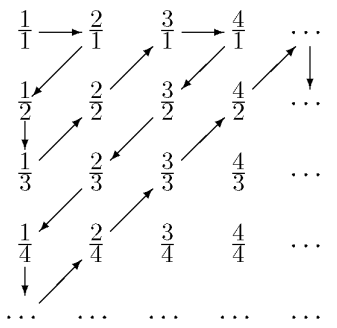
\includegraphics[width = 0.5\textwidth]{rational-numbers.png}
        \caption{Подсчёт обыкновенных дробей}
    \end{figure}

    $\mathbb{Q}^{+}$ -- бесконечное подмножество множества положительных обыкновенных дробей, которое
    счётно $\implies \mathbb{Q}^{+}$ счётно. $\blacksquare$

\newpage
\section{БИЛЕТ 2}

\subsection{Теорема Кантора о вложенных отрезках}

    \textbf{Теорема Кантора о вложенных отрезках}: Если $[a_1; b_1] \subset [a_2; b_2] \subset ...
    \subset [a_n; b_n] \subset ...$ -- бесконечная последовательность вложенных отрезков, то
    $\exists\gamma: \forall n \hookrightarrow a_n \leq \gamma \leq b_n$; если при этом
    $\lim\limits_{n\to \infty} (b_n - a_n) = 0$, то такая точка $\gamma$ единственна, и
    $\gamma = \lim\limits_{n\to\infty}a_n = \sup a_n = \lim\limits_{n\to\infty}b_n = \inf b_n$.

    $\square$ Так как $\forall n\in\mathbb{N} \hookrightarrow a_1 \leq a_2 \leq ... \leq a_n
    \leq ... \leq b_n \leq ... \leq b_2 \leq b_1$, то $\forall n, m\in\mathbb{N} \hookrightarrow
    a_n \leq b_m$.\\
    Рассмотрим множества $A = \{a_1, a_2, ..., a_n, ...\}$ и $B = \{b_1, b_2, ..., b_n, ...\}$.
    $\forall m\in\mathbb{N}$ множество $A$ ограничено сверху числом $b_m$ $\implies \exists
    \gamma_1 = \sup A = \sup a_n$. Так как $\forall m\in\mathbb{N} \hookrightarrow b_m$ -- верхняя
    граница множества $A$, то $\gamma_1 \leq b_m$. Аналогично множество $B$ ограничено снизу и
    $\exists \gamma_2 = \inf B = \inf b_n$; $\forall n\in\mathbb{N} \hookrightarrow a_n$ - нижняя
    граница $B$ $\implies \gamma_2 \geq a_n$. Так как $\gamma_2$ -- верхняя граница $a_n$, то
    $\gamma_2 \geq \sup a_n \implies \gamma_2 \geq \gamma_1$.\\
    Итак, $\forall n\in\mathbb{N} \hookrightarrow a_n \leq \gamma_1 \leq \gamma_2 \leq b_n$. Поэтому
    точки $\gamma_1$ и $\gamma_2$ (и весь отрезок $[\gamma_1; \gamma_2]$, если $\gamma_1 < \gamma_2$)
    принадлежат всем отрезкам $[a_n; b_n]$. Первая часть теоремы доказана.\\
    Пусть теперь $\lim\limits_{n\to \infty} (b_n - a_n) = 0$. Тогда $0 \leq |\gamma_2 - \gamma_1|
    \leq b_n - a_n$, и по теореме о двух милиционерах $\lim\limits_{n\to \infty} |\gamma_2 -
    \gamma_1| = 0 \implies |\gamma_2 - \gamma_1| = 0 \implies \gamma_1 = \gamma_2 = \gamma$. Тогда
    $\gamma = \sup a_n = \inf b_n$. Последовательность $a_n$ монотонно возрастает и ограничена сверху
    $\implies$ по теореме Вейерштрасса $\gamma = \lim\limits_{n\to\infty}a_n$. Аналогично $\gamma =
    \lim\limits_{n\to\infty}b_n$.\\
    Если $\exists\delta \neq \gamma: \forall n\in\mathbb{N} \hookrightarrow a_n \leq \delta
    \leq b_n$, то $|\gamma - \delta| \leq b_n - a_n \implies \delta = \gamma$. Единственность общей
    точки доказана. $\blacksquare$

    \textbf{Теорема о несчётности множества действительных чисел}: множество $\mathbb {R}$ является
    несчётным.

    $\square$ Докажем сначала несчётность множества чисел отрезка $[a; b]$. Предположим, что все
    точки отрезка удалось занумеровать в виде последовательности $x_1, x_2, ..., x_n, ...$  Пусть
    $[a_1; b_1] \subset [a; b]$ -- такой отрезок, что $x_1 \not\in [a_1; b_1]$; $[a_2; b_2] \subset
    [a_1; b_1]$ -- такой отрезок, что $x_2 \not\in [a_2; b_2]$ и т.д. Построенная последовательность
    вложенных отрезков имеет общую точку $\gamma$. Однако
    \begin{equation*}
        \forall n\in\mathbb{N} \hookrightarrow x_n \not\in [a_n; b_n] \implies x_n \neq \gamma
    \end{equation*}
    То есть $\gamma$ не является членом последовательности $x_n$ -- противоречие $\implies$ множество
    точек любого отрезка несчётно. Так как $[a; b] \subset \mathbb{R}$, то $\mathbb{R}$ также
    несчётно. $\blacksquare$

\newpage
\section{БИЛЕТ 3}

\subsection{Предел числовой последовательности}

    \textbf{Определение}: функцией $f$ с областью определения $X$ и областью значений из $Y$
    называется такое соответствие между $X$ и $Y$, что любому $x\in X$ соответствует единственный
    $y\in Y$.

    \textbf{Формальное определение}: бинарное отношение $f\subseteq X\times Y$ называется функцией,
    если из $(x, y)\in f$ и $(x, y')\in f$ следует, что $y = y'$.

    \textbf{Определение}: числовой последовательностью называется функция с областью определения
    $\mathbb{N}$ и множеством значений, принадлежащим $\mathbb{R}$.

    \textbf{Определение}: Пусть $E(f) \subseteq \mathbb{R}$. Функция $f$ называется ограниченной
    (ограниченной сверху/снизу) на множестве $X$, если $E(f)$ ограничено (ограничено сверху/снизу);
    точные верхняя и нижняя грани $E(f)$ называются точной верхней и нижней гранями $f$ на $X$ и
    обозначаются $\sup\limits_X f(x)$ и $\inf\limits_X f(x)$ соответственно. Числовая последовательность
    $x_n$ называется ограниченной (ограниченной сверху/снизу), если множество её значений ограничено
    (ограничено сверху/снизу); точные верхняя и нижняя грани этого множества называются точной
    верхней и нижней гранями $x_n$ и обозначаются $\sup x_n$ и $\inf x_n$ соответственно.

    \textbf{Лемма}: Функция $f(x)$ ограничена на множестве $X$ $\iff$ $\exists C > 0: \forall x\in X
    \hookrightarrow |f(x)| \leq C$.

    $\square$ $\boxed{\Leftarrow}$ $|f(x)| \leq C \iff -C \leq f(x) \leq C$. Так как это неравенство
    выполняется $\forall x$, то множество значений функции $f(x)$ ограничено.\\
    $\boxed{\Rightarrow}$ Функция ограничена на множестве $X$ $\implies\forall x\in X\hookrightarrow m
    \leq f(x) \leq M$, где $m = \inf\limits_X f(x)$, $M = \sup\limits_X f(x)$. Отсюда следует, что
    $|f(x)| \leq C$, где $C = max(|m|, |M|)$. $\blacksquare$

    \textbf{Определение}: $\varepsilon$-окрестностью $U_{\varepsilon}(\alpha)$ символа $\alpha$, где
    $\alpha$ -- один из 6 стандартных предельных символов $a$, $a + 0$, $a - 0$, $+\infty$, $-\infty$,
    $\infty$, называется одно из следующих 6 множеств:
    \begin{enumerate}
        \item $U_{\varepsilon}(a) = (a - \varepsilon; a + \varepsilon)$;
        \item $U_{\varepsilon}(a + 0) = [a; a + \varepsilon)$;
        \item $U_{\varepsilon}(a - 0) = (a - \varepsilon; a]$;
        \item $U_{\varepsilon}(+\infty) = (\varepsilon; +\infty)$;
        \item $U_{\varepsilon}(-\infty) = (-\infty; -\varepsilon)$;
        \item $U_{\varepsilon}(\infty) = (-\infty; -\varepsilon)\cup(\varepsilon; +\infty)$,
    \end{enumerate}
    где $a\in\mathbb{R}$, $\varepsilon > 0$.

    \textbf{Определение предела числовой последовательности}: символ $\alpha$ называется пределом
    числовой последовательности $x_n$, если
    \begin{equation*}
    \forall \varepsilon > 0 \hookrightarrow \exists n_0(\varepsilon)\in\mathbb{N}:
    \forall n \geq n_0 \hookrightarrow x_n\in U_{\varepsilon}(\alpha)
    \end{equation*}
    Обозначение предела: $\lim\limits_{n\to\infty} x_n = \alpha$.

    \textbf{Определение}: последовательность, имеющая конечный предел, называется сходящейся;
    последовательность, не имеющая конечного предела, называется расходящейся.

    \textbf{Лемма}: если последовательность $x_n$ ограничена при $n \geq n_0,\ n_0\in\mathbb{N}$ и
    определена $\forall n\in\mathbb{N}$, то она ограничена.

    $\square$ $x_n$ ограничена при $n \geq n_0,\ n_0\in\mathbb{N}$ $\iff$ $\exists m, M\in\mathbb{R}
    \forall n \geq n_0 \hookrightarrow m \leq x_n \leq M$. Вне отрезка $[m; M]$ имеется не более
    конечного числа членов последовательности $x_n$ (разве что $x_1, x_2, ..., x_{n_0 - 1}$).
    Рассмотрим $m_1 = min(x_1, x_2, ..., x_{n_0 - 1}, m)$, $M_1 = max(x_1, x_2, ..., x_{n_0 - 1}, M)$.
    Тогда $\forall n\in\mathbb{N} \hookrightarrow m_1 \leq x_n \leq M_1 \implies x_n$ ограничена.
    $\blacksquare$

    \textbf{Лемма}: сходящаяся последовательность ограничена.

    $\square$ Пусть $\lim\limits_{n\to\infty} x_n = a$. По определению предела последовательности
    при $\varepsilon = 1$:
    \begin{equation*}
    \exists n_0(\varepsilon)\in\mathbb{N}: \forall n \geq n_0 \hookrightarrow |x_n - a| < 1,
    \end{equation*}
    то есть $\forall n \geq n_0 \hookrightarrow a - 1 < x_n < a + 1$. Последовательность ограничена
    при $n \geq n_0 \implies$ последовательность ограничена. $\blacksquare$

\subsection{Единственность предела}

    \textbf{Лемма}: сходящаяся последовательность имеет единственный предел.

    $\square$ Пусть $\lim\limits_{n\to\infty} x_n = a$ и $\lim\limits_{n\to\infty} x_n = b$; для
    определённости $a < b$.\\
    Зафиксируем $\varepsilon > 0: U_{\varepsilon}(a)\cap U_{\varepsilon}(b) = \emptyset$, то есть
    $\varepsilon \leq \dfrac{b - a}{2}$. По определению предела:\\
    \begin{equation*}
        \exists n_1(\varepsilon)\in\mathbb{N}: \forall n\geq n_1 \hookrightarrow x_n\in U_{\varepsilon}(a)
    \end{equation*}
    \begin{equation*}
        \exists n_2(\varepsilon)\in\mathbb{N}: \forall n\geq n_2 \hookrightarrow x_n\in U_{\varepsilon}(b)
    \end{equation*}
    Тогда при $n \geq n_3 = max(n_1, n_2) \hookrightarrow x_n\in U_{\varepsilon}(a)\cap
    U_{\varepsilon}(b) = \emptyset$ -- противоречие. $\blacksquare$

\subsection{Бесконечно малые последовательности и их свойства}

    \textbf{Определение}: Последовательность называется бесконечно малой, если
    $\lim\limits_{n\to\infty} x_n = 0$.

    \textbf{Лемма}: $\lim\limits_{n\to\infty} x_n = a \iff x_n = a + \alpha_n$, где $\alpha_n$ --
    бесконечно малая последовательность.

    $\square$ Пусть $\alpha_n = x_n - a$, тогда:
    \begin{equation*}
    \lim\limits_{n\to\infty} x_n = a \iff \forall\varepsilon > 0 \hookrightarrow \exists
    n_0(\varepsilon)\in\mathbb{N}: \forall n \geq n_0 \hookrightarrow |x_n - a| < \varepsilon \iff
    \end{equation*}
    \begin{equation*}
    \iff \forall\varepsilon > 0 \hookrightarrow \exists n_0(\varepsilon)\in\mathbb{N}: \forall n
    \geq n_0 \hookrightarrow |\alpha_n| < \varepsilon \iff \lim\limits_{n\to\infty} \alpha_n = 0
    \end{equation*}
    $\blacksquare$

    \textbf{Лемма}: сумма двух бесконечно малых последовательностей является бесконечно малой
    последовательностью.

    $\square$ Пусть $\alpha_n$ и $\beta_n$ -- бесконечно малые последовательности. Тогда:
    \begin{equation*}
        \forall\varepsilon > 0 \hookrightarrow \exists n_1(\varepsilon)\in\mathbb{N}: \forall n
        \geq n_1 \hookrightarrow |\alpha_n| < \dfrac{\varepsilon}{2}
    \end{equation*}
    \begin{equation*}
        \forall\varepsilon > 0 \hookrightarrow \exists n_2(\varepsilon)\in\mathbb{N}: \forall n
        \geq n_2 \hookrightarrow |\beta_n| < \dfrac{\varepsilon}{2}
    \end{equation*}
    Тогда при $n \geq n_0 = max(n_1, n_2)$ выполняется $|\alpha_n + \beta_n|\leq |\alpha_n| +
    |\beta_n| < \dfrac{\varepsilon}{2} + \dfrac{\varepsilon}{2} = \varepsilon$, то есть $\alpha_n +
    \beta_n$ -- бесконечно малая. $\blacksquare$

    \textbf{Лемма}: произведение бесконечно малой последовательности на ограниченную является
    бесконечно малой последовательностью.

    $\square$ Если последовательность $\beta_n$ ограничена, то $\exists C > 0:
    \forall n\in\mathbb{N} \hookrightarrow |\beta_n|\leq C$. Если $\alpha_n$ -- бесконечно малая, то
    \begin{equation*}
        \forall\varepsilon > 0 \hookrightarrow \exists n_0(\varepsilon)\in\mathbb{N}: \forall n
        \geq n_0 \hookrightarrow |\alpha_n| < \dfrac{\varepsilon}{C}
    \end{equation*}
    Тогда при $n \geq n_0$ выполняется $|\alpha_n\beta_n| < \dfrac{\varepsilon}{C}\cdot C =
    \varepsilon$, то есть $\alpha_n\beta_n$ -- бесконечно малая. $\blacksquare$

    \textbf{Следствие 1}: если $\alpha_n$ -- бесконечно малая последовательность, $C\in\mathbb{R}$,
    то $x_n = C\alpha_n$ -- бесконечно малая последовательность.

    $\square$ Следует из того, что постоянная последовательность ограничена. $\blacksquare$

    \textbf{Следствие 2}: произведение двух бесконечно малых последовательностей является бесконечно
    малой последовательностью.

    $\square$ Следует из того, что одну из последовательностей можно рассматривать как имеющую
    конечный предел, следовательно, ограниченную. $\blacksquare$

\subsection{Свойства пределов, связанные с неравенствами}

    \textbf{Усиленная лемма о сохранении знака}: если $\lim\limits_{n\to\infty} x_n = a$, где
    $a \neq 0$, то
    \begin{equation*}
    \exists n_0\in\mathbb{N}: \forall n \geq n_0 \hookrightarrow |x_n| > \dfrac{|a|}{2},\
    sign(x_n) = sign(a)
    \end{equation*}

    $\square$ Пусть $a > 0$. Зафиксируем в определении предела $\varepsilon = \dfrac{a}{2}$, тогда:
    \begin{equation*}
        \exists n_1\in\mathbb{N}: \forall n \geq n_1 \hookrightarrow |x_n - a| < \dfrac{a}{2}
    \end{equation*}
    Следовательно, $x_n > \dfrac{a}{2}$. В качестве $n_0$ можно рассмотреть любое $n\in\mathbb{N}:
    n \geq n_1$. Случай $a < 0$ рассматривается аналогично $\left(\text{в определении предела берётся }
    \varepsilon = \dfrac{|a|}{2}\right)$. $\blacksquare$

    \textbf{Лемма о сохранении знака}: если $\lim\limits_{n\to\infty} x_n = a$, где $a \neq 0$, то
    \begin{equation*}
        \exists n_0\in\mathbb{N}: \forall n \geq n_0 \hookrightarrow sign(x_n) = sign(a)
    \end{equation*}

    $\square$ Напрямую следует из усиленной леммы о сохранении знака. $\blacksquare$

    \textbf{Теорема о предельном переходе в неравенстве}: если $\lim\limits_{n\to\infty} x_n = a$,
    $\lim\limits_{n\to\infty} y_n = b$, причём $\exists n_0\in\mathbb{N}: \forall n \geq n_0
    \hookrightarrow x_n \leq y_n$, то $a \leq b$.

    $\square$ Предположим, что $a > b$. Рассмотрим $\varepsilon > 0: U_{\varepsilon}(a)\cap
    U_{\varepsilon}(b) = \emptyset \left(\text{например, }\varepsilon = \dfrac{a - b}{2}\right)$,
    тогда:
    \begin{equation*}
        \exists n_1(\varepsilon)\in\mathbb{N}: \forall n\geq n_1 \hookrightarrow x_n\in
        U_{\varepsilon}(a)
    \end{equation*}
    \begin{equation*}
        \exists n_2(\varepsilon)\in\mathbb{N}: \forall n\geq n_2 \hookrightarrow y_n\in
        U_{\varepsilon}(b)
    \end{equation*}
    При $n \geq n_3 = max(n_0, n_1, n_2)$ выполняется $x_n > y_n$, что противоречит условию.
    $\blacksquare$

    \textit{Замечание}: если $\lim\limits_{n\to\infty} x_n = a$, $\lim\limits_{n\to\infty} y_n = b$,
    причём $\exists n_0\in\mathbb{N}: \forall n \geq n_0 \hookrightarrow x_n < y_n$, то $a \leq b$
    (возможно $a = b$). Например: $x_n = -\dfrac{1}{n} < y_n = \dfrac{1}{n}; \lim\limits_{n\to\infty}
    x_n = \lim\limits_{n\to\infty} y_n = 0$.

    \textbf{Следствие}: если $\exists n_0\in\mathbb{N}: \forall n \geq n_0 \hookrightarrow x_n \in
    [a; b]$ и $\lim\limits_{n\to\infty} x_n = c$, то $c \in [a; b]$.

    $\square$
    \begin{equation*}
        \forall n \geq n_0\in\mathbb{N} \hookrightarrow x_n \geq a \implies c \geq a
    \end{equation*}
    \begin{equation*}
        \forall n \geq n_0\in\mathbb{N} \hookrightarrow x_n \leq b \implies c \leq b
    \end{equation*}
    Тогда $(c \geq a) \wedge (c \leq b) \implies c \in [a; b].$ $\blacksquare$

    \textbf{Теорема о двух милиционерах}: если $\lim\limits_{n\to\infty} x_n =
    \lim\limits_{n\to\infty} z_n = a$ и
    \begin{equation*}
        \exists n_0\in\mathbb{N}: \forall n \geq n_0 \hookrightarrow x_n \leq y_n \leq z_n,
    \end{equation*}
    то $\lim\limits_{n\to\infty} y_n = a$.

    $\square$ По определению предела числовой последовательности:
    \begin{equation*}
        \forall \varepsilon > 0 \hookrightarrow \exists n_1(\varepsilon)\in\mathbb{N}: \forall n
        \geq n_1 \hookrightarrow x_n\in U_{\varepsilon}(a)
    \end{equation*}
    \begin{equation*}
        \forall \varepsilon > 0 \hookrightarrow \exists n_2(\varepsilon)\in\mathbb{N}: \forall n
        \geq n_2 \hookrightarrow z_n\in U_{\varepsilon}(a)
    \end{equation*}
    Тогда $\forall n \geq n_3 = max(n_0, n_1, n_2) \hookrightarrow a - \varepsilon < x_n \leq y_n
    \leq z_n < a + \varepsilon$, то есть
    \begin{equation*}
        \forall \varepsilon > 0 \hookrightarrow \exists n_3(\varepsilon)\in\mathbb{N}: \forall n
        \geq n_3 \hookrightarrow y_n\in U_{\varepsilon}(a)
    \end{equation*}
    Значит, $\lim\limits_{n\to\infty} y_n = a$. $\blacksquare$\\

    \subsection{Арифметические операции со сходящимися последовательностями}
    \textbf{Теорема}: пусть $\lim\limits_{n\to\infty} x_n = a\in\mathbb{R}$,
    $\lim\limits_{n\to\infty} y_n = b\in\mathbb{R}$, тогда:
    \begin{enumerate}
        \item $\lim\limits_{n\to\infty} (x_n + y_n) = a + b$;
        \item $\lim\limits_{n\to\infty} (x_n\cdot y_n) = ab$;
        \item Если $b \neq 0$, то $\lim\limits_{n\to\infty} \dfrac{x_n}{y_n} = \dfrac{a}{b}$.
    \end{enumerate}

    $\square$ $x_n = a + \alpha_n$, $y_n = b + \beta_n$, где $\alpha_n$, $\beta_n$ - бесконечно малые
    последовательности.

    1) $x_n + y_n = (a + \alpha_n) + (b + \beta_n) = (a + b) + (\alpha_n + \beta_n)$.

    $\alpha_n + \beta_n$ -- бесконечно малая как сумма двух бесконечно малых
    $\implies$$\lim\limits_{n\to\infty} (x_n + y_n) = a + b$.

    2) $x_n\cdot y_n = (a + \alpha_n)(b + \beta_n) = ab + (a\beta_n + b\alpha_n + \alpha_n\beta_n)$.

    $a\beta_n + b\alpha_n + \alpha_n\beta_n$ -- бесконечно малая как сумма двух произведений
    бесконечно малой на константу и произведения двух бесконечно малых $\implies
    \lim\limits_{n\to\infty} (x_n\cdot y_n) = ab$.

    3) Так как $b \neq 0$, то по лемме о сохранении знака
    \begin{equation*}
        \exists n_0\in\mathbb{N}: \forall n \geq n_0 \hookrightarrow y_n \neq 0
    \end{equation*}
    Значит, $\dfrac{x_n}{y_n}$ определена $\forall n \geq n_0$ и не нужно требовать $y_n \neq 0$.
    \begin{equation*}
        \dfrac{x_n}{y_n} - \dfrac{a}{b} = \dfrac{a + \alpha_n}{b + \beta_n} - \dfrac{a}{b} =
        \dfrac{ab + b\alpha_n - ab - a\beta_n}{b(b + \beta_n)} =
        \dfrac{b\alpha_n - a\beta_n}{b(b +\beta_n)} = \dfrac{1}{y_n}
        \left(\alpha_n - \dfrac{a}{b}\beta_n\right)
    \end{equation*}
    $\alpha_n - \dfrac{a}{b}\beta_n$ -- бесконечно малая как сумма бесконечно малой и произведения
    бесконечно малой на константу. Так как $b \neq 0$, то по усиленной лемме о сохранении знака
    \begin{equation*}
        \exists n_1\in\mathbb{N}: \forall n \geq n_1 \hookrightarrow |y_n| > \dfrac{|b|}{2} \implies
        \dfrac{1}{|y_n|} < \dfrac{2}{|b|}
    \end{equation*}
    Значит, $\dfrac{1}{y_n}$ ограничена при $n \geq n_1 \implies \dfrac{1}{y_n}$ ограничена.
    Таким образом, $\dfrac{1}{y_n}(\alpha_n - \dfrac{a}{b}\beta_n)$ -- бесконечно малая $\implies
    \lim\limits_{n\to\infty} \dfrac{x_n}{y_n} = \dfrac{a}{b}$. $\blacksquare$

    \textbf{Следствия (в обозначениях теоремы)}:
    \begin{enumerate}
        \item $\lim\limits_{n\to\infty} Cx_n = Ca$;
        \item $\lim\limits_{n\to\infty} (x_n - y_n) = a - b$;
        \item $\lim\limits_{n\to\infty} x_{n}^{k} = {a}^k$ (при $k\in\mathbb{N}$; если $a \neq 0$,
              то при $k\in\mathbb{Z}$);
        \item $\lim\limits_{n\to\infty} \dfrac{1}{n^k} = 0$ (при $k\in\mathbb{N}$), так как
              $\dfrac{1}{n^k} = \left(\dfrac{1}{n}\right)^k$ и $\lim\limits_{n\to\infty} \dfrac{1}{n}
              = 0$.
    \end{enumerate}

\subsection{Теорема Вейерштрасса о пределе монотонной ограниченной последовательности}

    \textbf{Определение}: последовательность $x_n$ называется
    \begin{enumerate}
        \item строго возрастающей, если $\forall n\in\mathbb{N} \hookrightarrow x_{n+1} > x_n$;
        \item строго убывающей, если $\forall n\in\mathbb{N} \hookrightarrow x_{n+1} < x_n$;
        \item нестрого возрастающей, если $\forall n\in\mathbb{N} \hookrightarrow x_{n+1} \geq x_n$;
        \item нестрого убывающей, если $\forall n\in\mathbb{N} \hookrightarrow x_{n+1} \leq x_n$;
    \end{enumerate}
    все такие последовательности называются монотонными.

    \textbf{Теорема Вейерштрасса}: если последовательность $x_n$ возрастает (строго или нестрого) и
    ограничена сверху, то $\exists\lim\limits_{n\to\infty} x_n = \sup x_n$; если последовательность
    $x_n$ убывает (строго или нестрого) и ограничена снизу, то $\exists\lim\limits_{n\to\infty}
    x_n = \inf x_n$.

    $\square$ Докажем первую часть теоремы. Вторая доказывается аналогично.\\
    По теореме о точной верхней грани $\exists\sup x_n = \alpha$. Тогда
    \begin{equation*}
        (\forall n\in\mathbb{N} \hookrightarrow x_n \leq \alpha)\wedge
        (\forall \alpha' < a \hookrightarrow \exists n_0(\alpha')\in\mathbb{N}: x_{n_0} > \alpha')
    \end{equation*}
    Введём обозначение: $\varepsilon = \alpha - \alpha'$, $\varepsilon > 0$. Последовательность
    $x_n$ монотонно возрастает, следовательно:
    \begin{equation*}
        \forall n \geq n_0 \hookrightarrow x_n \geq x_{n_0}
    \end{equation*}
    При этом также $x_n \leq \alpha$. Таким образом,
    \begin{equation*}
        \forall\varepsilon > 0 \hookrightarrow\exists n_0(\varepsilon(\alpha'))\in\mathbb{N}:
        \forall n \geq n_0 \hookrightarrow  \alpha- \varepsilon < x_{n_0} \leq x_n \leq \alpha
        \implies x_n\in U_{\varepsilon}(\alpha)
    \end{equation*}
    Отсюда следует, что $\lim\limits_{n\to\infty} x_n = \alpha = \sup x_n$. $\blacksquare$

\subsection{Число $e$}

    \textbf{Определение}: числом $e$ называется предел $\lim\limits_{n\to\infty}
    \left(1 + \dfrac{1}{n}\right)^n$.

    $\square$ Докажем корректность этого определения, то есть докажем существование такого предела.
    Пусть $x_n = \left(1 + \dfrac{1}{n}\right)^n$. Рассмотрим последовательность
    $y_n = \left(1 + \dfrac{1}{n}\right)^{n+1} = x_n\left(1 + \dfrac{1}{n}\right)$. Докажем, что
    $\exists\lim\limits_{n\to\infty} y_n$.
    \begin{equation*}
        \dfrac{y_n}{y_{n+1}} = \dfrac{(n+1)^{n+1}\cdot (n+1)^{n+2}}{n^{n+1}\cdot(n+2)^{n+2}} =
        \dfrac{(n+1)^{2n + 4}}{(n(n+2))^{n+2}}\cdot\dfrac{n}{n+1} =
        \left(\dfrac{n^2 + 2n + 1}{n^2 + 2n}\right)^{n + 2}\cdot\dfrac{n}{n+1} =
    \end{equation*}
    \begin{equation*}
        = \left(1 + \dfrac{1}{n^2 + 2n}\right)^{n+2}\cdot\dfrac{n}{n+1} \geq
        \left(1 + \dfrac{n+2}{n^2 + 2n}\right)\cdot\dfrac{n}{n+1} =
        \left(1 + \dfrac{1}{n}\right)\cdot\dfrac{n}{n+1} = 1
    \end{equation*}
    Итак, $y_{n+1} \leq y_n \implies$ последовательность $y_n$ нестрого убывает. Также
    $\forall n\in\mathbb{N} \hookrightarrow y_n > 1$. По теореме Вейерштрасса,
    $\lim\limits_{n\to\infty} y_n = \inf y_n$.
    \begin{equation*}
        x_n = \dfrac{y_n}{1 + \dfrac{1}{n}} \implies \lim\limits_{n\to\infty} x_n =
        \dfrac{\lim\limits_{n\to\infty} y_n}{\lim\limits_{n\to\infty} \left(1 + \dfrac{1}{n}\right)} =
        \dfrac{\lim\limits_{n\to\infty} y_n}{1} = \lim\limits_{n\to\infty} y_n
    \end{equation*}
    Обозначим $\lim\limits_{n\to\infty} x_n = \lim\limits_{n\to\infty} y_n = e$. $\blacksquare$

\subsection{Бесконечно малые и бесконечно большие последовательности и их свойства}

    \textbf{Определение}: последовательность $x_n$ называется бесконечно большой, если
    $\lim\limits_{n\to\infty} x_n = \infty$.

    \textbf{Лемма}: бесконечно большая последовательность является неограниченной.

    $\square$ Если $x_n$ неограниченна, то:
    \begin{equation*}
        \forall E > 0 \hookrightarrow \exists n(E)\in\mathbb{N}: |x_n| > E
    \end{equation*}
    Если $x_n$ является бесконечно большой, то:
    \begin{equation*}
        \forall E > 0 \hookrightarrow \exists n_0(E)\in\mathbb{N}: \forall n \geq n_0
        \hookrightarrow |x_n| > E
    \end{equation*}
    Условию неограниченности, например, удовлетворяет $n_0$, поэтому бесконечно большая
    последовательность неограниченна. $\blacksquare$

    \textbf{Лемма}: 1) если последовательность $x_n$ является бесконечно большой, то
    последовательность $y_n = \dfrac{1}{x_n}$ -- бесконечно малая;\\
    2) если последовательность $x_n$ бесконечно малая, и $\exists n_0\in\mathbb{N}: \forall n \geq
    n_0 \hookrightarrow x_n \neq 0$, то последовательность $y_n = \dfrac{1}{x_n}$ -- бесконечно
    большая.

    $\square$ По определению бесконечно большой последовательности:
    \begin{equation*}
        \forall E > 0 \hookrightarrow \exists n_0(E)\in\mathbb{N}: \forall n \geq n_0
        \hookrightarrow |x_n| > E
    \end{equation*}
    Тогда по $\forall n \geq n_0 \hookrightarrow x_n \neq 0 \implies$ последовательность $y_n$
    определена, и не нужно делать дополнительную оговорку, как во второй части леммы. $\forall E$
    рассмотрим $\varepsilon = \dfrac{1}{E}$. Тогда:
    \begin{equation*}
        \forall \varepsilon > 0 \hookrightarrow \exists n_0(\varepsilon(E))\in\mathbb{N}: \forall n
        \geq n_0 \hookrightarrow |x_n| > E \implies |y_n| = \dfrac{1}{|x_n|} < \dfrac{1}{E} =
        \varepsilon \implies \lim\limits_{n\to\infty} y_n = 0
    \end{equation*}
    То есть $y_n$ -- бесконечно малая.

    2) Доказательство аналогично. $\blacksquare$

    \textbf{Лемма}: 1) если $\lim\limits_{n\to\infty} x_n = +\infty$ и $\exists n_0\in\mathbb{N}:
    \forall n \geq n_0 \hookrightarrow y_n \geq x_n$, то $\lim\limits_{n\to\infty} y_n = +\infty$;\\
    2) если $\lim\limits_{n\to\infty} x_n = -\infty$ и $\exists n_0\in\mathbb{N}: \forall n \geq
    n_0 \hookrightarrow y_n \leq x_n$, то $\lim\limits_{n\to\infty} y_n = -\infty$.

    $\square$ 1) Так как $\lim\limits_{n\to\infty} x_n = +\infty$, то
    \begin{equation*}
        \forall E > 0 \hookrightarrow\exists n_1(E)\in\mathbb{N}: \forall n \geq n_1
        \hookrightarrow x_n > E
    \end{equation*}
    Пусть $n_2 = max(n_0, n_1)$, тогда
    \begin{equation*}
        \forall n \geq n_2 \hookrightarrow y_n \geq x_n > E \implies \lim\limits_{n\to\infty} y_n =
        +\infty
    \end{equation*}

    2) Доказательство аналогично. $\blacksquare$

    \textbf{Аналог теоремы Вейерштрасса для бесконечно больших последовательностей}:

    1) если последовательность $x_n$ возрастает (строго или нестрого) и неограниченна сверху, то
    \begin{equation*}
        \lim\limits_{n\to\infty} x_n = +\infty
    \end{equation*}

    2) если последовательность $x_n$ убывает (строго или нестрого) и неограниченна снизу, то
    \begin{equation*}
        \lim\limits_{n\to\infty} x_n = -\infty
    \end{equation*}

    $\square$ Докажем первую часть теоремы, вторая доказывается аналогично.

    Так как $x_n$ неограниченна сверху, то
    \begin{equation*}
        \forall E > 0 \hookrightarrow \exists n_0(E)\in\mathbb{N}: x_{n_0} > E
    \end{equation*}
    Последовательность монотонно возрастает $\implies \forall n \geq n_0 \hookrightarrow x_n\geq
    x_{n_0}$. Поэтому:
    \begin{equation*}
        \forall E > 0 \hookrightarrow \exists n_0(E)\in\mathbb{N}: \forall n \geq n_0
        \hookrightarrow x_n > E
    \end{equation*}
    Значит, $\lim\limits_{n\to\infty} x_n = +\infty$. $\blacksquare$

\newpage
\section{БИЛЕТ 4}

\subsection{Подпоследовательности, частичные пределы}

    \textbf{Определение}: пусть $x_n$ -- числовая последовательность, а $n_k$ -- строго возрастающая
    последовательность натуральных чисел, тогда последовательность $y_k = x_{n_k}$ называется
    подпоследовательностью последовательности $x_n$.

    \textbf{Определение}: число $a\in\mathbb{R}$ (или символ $+\infty$, $-\infty$) называется
    частичным пределом (предельной точкой) последовательности $x_n$, если существует такая строго
    возрастающая последовательность индексов $n_k$, что $\lim\limits_{k\to\infty} x_{n_k} = a$.

    \textbf{Лемма}: если $\lim\limits_{n\to\infty} x_n = \alpha$, где $\alpha$ -- один из 6 СПС, то
    $\forall x_{n_k} \hookrightarrow \lim\limits_{k\to\infty} x_{n_k} = \alpha$.

    $\square$ По определению предела, вне любой окрестности $U_{\varepsilon}(\alpha)$ содержится не
    более конечного числа членов $x_n$. Так как все $n_k$ различны, то вне любой
    $U_{\varepsilon}(\alpha)$ имеется не более конечного числа членов $x_{n_k} \implies
    \lim\limits_{k\to\infty} x_{n_k} = \alpha$. $\blacksquare$

    \textbf{Следствие}: если  $\lim\limits_{n\to\infty} x_n = a\in\mathbb{R}$, то $a$ -- единственный
    частичный предел $x_n$.

    $\square$ Так как все подпоследовательности имеют один и тот же предел, то он является единственным
    частичным пределом. $\blacksquare$

    \textbf{Критерий частичного предела}: пусть $\alpha$ -- один из символов $a$, $+\infty$, $-\infty$,
    тогда $\alpha$ является частичным пределом $\iff$ в любой $U_{\varepsilon}(\alpha)$ содержится
    бесконечно много членов $x_n$.

    $\square$ $\boxed{\Rightarrow}$ Если $\alpha$ -- частичный предел $x_n$, то существует подпоследовательность
    $x_{n_k}: \lim\limits_{k\to\infty} x_{n_k} = \alpha$. Тогда $\forall \varepsilon > 0$ внутри
    $U_{\varepsilon}(\alpha)$ содержатся все $x_{n_k}$, начиная с некоторого номера $k_0$, а значит,
    бесконечно много членов $x_n$.

    $\boxed{\Leftarrow}$ Сначала рассмотрим случай $a\in\mathbb{R}$. Возьмём $\varepsilon = 1$, $x_{n_1}$
    - некоторый член $x_n$ из $U_{1}(a)$. Возьмём теперь $\varepsilon = \dfrac{1}{2}$. Так как в
    $U_{\frac{1}{2}}(a)$ бесконечно много членов, то выберем $x_{n_2}\in U_{\frac{1}{2}}(a)$ так,
    что $n_2 > n_1$, и т.д. Пусть построены $x_{n_1}, x_{n_2}, ..., x_{n_k}$, где
    $n_1 < n_2 < ... < n_k$, $x_{n_k}\in U_{\frac{1}{k}}(a)$. Так как в $U_{\frac{1}{k+1}}(a)$
    бесконечно много членов $x_n$, то выберем $x_{k+1}\in U_{\frac{1}{k+1}}(a)$ так, чтобы
    $n_{k+1} > n_k$. Таким образом, построена бесконечная последовательность $x_{n_k}$, причём
    $n_1 < n_2 < ... < n_k < ...$, $\forall k\in\mathbb{N} \hookrightarrow x_{n_k}\in U_{\frac{1}{k}}(a)$.
    То есть $\forall k\in\mathbb{N} \hookrightarrow a - \dfrac{1}{k} < x_{n_k} < a + \dfrac{1}{k}$.
    По теореме о двух милиционерах: $\lim\limits_{k\to\infty} x_{n_k} = a$, то есть $a$ -- частичный
    предел $x_n$.

    Для $\alpha = +\infty$ и $\alpha = -\infty$ доказательство аналогично. Например, для
    $\alpha = +\infty$ нужно брать $\varepsilon = 1, 2, 3, ..., k, ...$; $x_{n_k}$ выбирать таким,
    что $x_{n_k}\in U_{k}(+\infty)$, то есть $x_{n_k} > k$. Тогда по аналогу теоремы о двух
    милиционерах для бесконечно больших последовательностей, $\lim\limits_{k\to\infty} x_{n_k} =
    +\infty$. $\blacksquare$

\subsection{Теорема Больцано-Вейерштрасса}

    \textbf{Теорема Больцано-Вейерштрасса}: любая ограниченная последовательность имеет сходящуюся
    подпоследовательность (то есть имеет конечный частичный предел).

    $\square$ Пусть $\forall n\in\mathbb{N} \hookrightarrow a \leq x_n \leq b$, где $a < b,
    a\in\mathbb{R}, b\in\mathbb{R}$. Выберем ту половину $\left[a; \dfrac{a + b}{2}\right]$ или
    $\left[\dfrac{a + b}{2}; b\right]$ отрезка $[a; b]$ (назовём её $\Delta_1$), где содержится
    бесконечно много $x_n$ (в обоих половинах конечного числа быть не может, так как в таком случае
    весь отрезок содержит конечное число членов последовательности, что неверно). Если обе половины
    содержат бесконечно много членов $x_n$, то $\Delta_1$ -- любая из половин. На отрезке $\Delta_1$
    аналогично выбираем половину $\Delta_2$, содержащую бесконечно много членов $x_n$, и т.д. На
    $k$-м шагу в $\Delta_k$ выбираем половину $\Delta_{k+1}$, содержащую бесконечно много членов
    $x_n$. Имеем последовательность вложенных отрезков $\Delta_1 \supset \Delta_2 \supset ...\supset
    \Delta_n \supset ...$, причём длина $n$-го отрезка равна $\dfrac{b-a}{2^n} =
    (b - a)\left(\dfrac{1}{2}\right)^n$ и стремится к нулю $(\lim\limits_{n\to\infty} \Delta_n = 0)$.
    По теореме Кантора о вложенных отрезка, $\exists! c: \forall n\in\mathbb{N} \hookrightarrow
    c\in\Delta_n$. Отсюда следует:
    \begin{equation*}
        \forall\varepsilon > 0 \hookrightarrow \exists n_0(\varepsilon)\in\mathbb{N}: \forall n \geq
        n_0 \hookrightarrow \Delta_n < \varepsilon \implies
        \forall n \geq n_0 \hookrightarrow \Delta_n \subset U_{\varepsilon}(c)
    \end{equation*}
    Значит, $U_{\varepsilon}(c)$ содержит бесконечно много членов $x_n$ $\implies$ по критерию
    частичного предела, $c$ -- частичный предел $x_n$. $\blacksquare$

    \textbf{Аналог теоремы Больцано-Вейерштрасса для неограниченных последовательностей}: если
    последовательность $x_n$ неограниченна сверху, то она имеет частичный предел $+\infty$; если
    последовательность $x_n$ неограниченна снизу, то она имеет частичный предел $-\infty$.

    $\square$ Докажем первую часть теоремы. Вторая доказывается аналогично.

    Зафиксируем $E > 0$. $x_n$ неограниченна $\implies \exists n_1(E)\in\mathbb{N}: x_{n_1} > E$.
    Теперь в качестве нового $E$ в определении неограниченности сверху рассмотрим $x_{n_1}$. Тогда
    $\exists n_2(x_{n_1})\in\mathbb{N}: x_{n_2} > x_{n_1}$ и т.д. Мы выбрали бесконечно много
    различных членов последовательности $x_n$ таких, что

    $x_{n_1} < x_{n_2} < ... < x_{n_k} < ...$ и $\forall k\in\mathbb{N} \hookrightarrow
    x_{n_k}\in U_{E}(+\infty) \implies$ по критерию частичного предела, $+\infty$ -- частичный предел
    последовательности $x_n$. $\blacksquare$

    \textbf{Теорема о единственном частичном пределе}: пусть последовательность $x_n$ ограничена и
    имеет единственный частичный предел, тогда $\lim\limits_{n\to\infty} x_n = a$.\\
    $\square$ Пусть $\forall n\in\mathbb{N} \hookrightarrow m
    \leq x_n \leq M$, где $m < M$, $m\in\mathbb{R}$, $M\in\mathbb{R}$. Так как для некоторой
    подпоследовательности $x_{n_k} \hookrightarrow \lim\limits_{k\to\infty} x_{n_k} = a$, и
    $\forall k \hookrightarrow m \leq x_{n_k} \leq M$, то по теореме о предельном переходе в
    неравенстве: $m \leq a \leq M$.

    Докажем, что $\exists\lim\limits_{n\to\infty} x_n = a$. Если это не так, то
    $\exists\varepsilon > 0:$ вне $U_{\varepsilon}(a)$ содержится бесконечно много членов $x_n$.
    Пусть для определённости бесконечно много членов $x_n$ справа от $U_{\varepsilon}(a)$, то есть
    на $[a + \varepsilon; M]$. По теореме Больцано-Вейерштрасса, на $[a + \varepsilon; M]$
    существует частичный предел $x_n$, отличный от $a$ -- противоречие. $\blacksquare$

\subsection{Критерий Коши существования конечного предела числовой последовательности}

    \textbf{Определение}: последовательность $x_n$ называется фундаментальной, если
    \begin{equation*}
        \forall\varepsilon > 0 \hookrightarrow \exists n_0(\varepsilon)\in\mathbb{N}: \forall n, m
        \geq n_0 \hookrightarrow |x_n - x_m| < \varepsilon
    \end{equation*}

    \textbf{Критерий Коши сходимости последовательности}: последовательность $x_n$ сходится $\iff$
    $x_n$ фундаментальна.

    $\square$ $\boxed{\Rightarrow}$ Пусть $\lim\limits_{n\to\infty} x_n = a\in\mathbb{R}$, тогда
    \begin{equation*}
        \forall\varepsilon > 0 \hookrightarrow \exists n_0(\varepsilon)\in\mathbb{N}: \forall n \geq
        n_0 \hookrightarrow |x_n - a| < \dfrac{\varepsilon}{2}
    \end{equation*}
    \begin{equation*}
        \forall\varepsilon > 0 \hookrightarrow \exists n_0(\varepsilon)\in\mathbb{N}: \forall m \geq
        n_0 \hookrightarrow |x_m - a| < \dfrac{\varepsilon}{2}
    \end{equation*}
    Тогда $\forall n, m \geq n_0$ выполняется
    \begin{equation*}
        |x_n - x_m| = |x_n - a + a - x_m| \leq |x_n - a| + |x_m - a| < \dfrac{\varepsilon}{2} +
        \dfrac{\varepsilon}{2} = \varepsilon.
    \end{equation*}
    Значит, последовательность $x_n$ фундаментальна.

    $\boxed{\Leftarrow}$ Пусть $x_n$ -- фундаментальная последовательность. Докажем сначала, что она
    ограничена. При $\varepsilon = 1$ имеем
    \begin{equation*}
        \exists n_0(1)\in\mathbb{N}: \forall n, m \geq n_0 \hookrightarrow |x_n - x_m| < 1
    \end{equation*}
    Зафиксируем $m = n_0$. Тогда
    \begin{equation*}
        \forall n \geq n_0 \hookrightarrow |x_n| = |x_n - x_m + x_m| \leq |x_n - x_m| + |x_m| <
        1 + |x_m| = 1 + |x_{n_0}|
    \end{equation*}
    Таким образом, последовательность $x_n$ ограничена при $n \geq n_0 \implies x_n$ ограничена.

    По теореме Больцано-Вейерштрасса последовательность $x_n$ имеет конечный частичный предел. В
    силу теоремы о единственном частичном пределе достаточно доказать, что других частичных пределов
    последовательность не имеет. Предположим, что это не так и существуют два различных частичных
    предела $a$ и $b$ (для определённости $a < b$). Возьмём в определении фундаментальности
    $\varepsilon = \dfrac{b - a}{3}$. Тогда для данного $\varepsilon$:
    \begin{equation*}
        \exists n_0\left(\dfrac{b - a}{3}\right)\in\mathbb{N}: \forall n, m \geq n_0
        \hookrightarrow|x_n - x_m| < \dfrac{b - a}{3}
    \end{equation*}
    В $U_{\varepsilon}(a)$ содержится бесконечно много членов $x_n$ по критерию частичного предела.
    Значит:
    \begin{equation*}
        \exists n_1\in\mathbb{N}, n_1 \geq n_0: x_{n_1}\in U_{\varepsilon}(a)
    \end{equation*}
    Аналогично:
    \begin{equation*}
        \exists n_2\in\mathbb{N}, n_2 \geq n_0: x_{n_2}\in U_{\varepsilon}(b)
    \end{equation*}
    Тогда $|x_{n_1} - x_{n_2}| > \dfrac{b - a}{3}$ -- противоречие определению фундаментальности.
    $\blacksquare$

\newpage
\section{БИЛЕТ 5}

\subsection{Определения предела числовой функции одной переменной по Коши и по Гейне, их эквивалентность}

    \textbf{Определение}: проколотой $\varepsilon$-окрестностью $\mathring U_{\varepsilon}(\alpha)$
    символа $\alpha$, где $\alpha$ -- один из 6 стандартных предельных символов ($a$, $a + 0$,
    $a - 0$, $+\infty$, $-\infty$, $\infty$), называется одно из следующих 6 множеств:
    \begin{enumerate}
        \item $\mathring U_{\varepsilon}(a) = (a - \varepsilon; a)\cup(a; a + \varepsilon)$;
        \item $\mathring U_{\varepsilon}(a + 0) = (a; a + \varepsilon)$;
        \item $\mathring U_{\varepsilon}(a - 0) = (a - \varepsilon; a)$;
        \item $\mathring U_{\varepsilon}(+\infty) = (\varepsilon; +\infty)$;
        \item $\mathring U_{\varepsilon}(-\infty) = (-\infty; -\varepsilon)$;
        \item $\mathring U_{\varepsilon}(\infty) = (-\infty; -\varepsilon)\cup(\varepsilon; +\infty)$,
    \end{enumerate}
    где $a\in\mathbb{R}, \varepsilon > 0$.

    \textbf{Определение предела функции по Гейне}: пусть функция $f$ определена в некоторой
    проколотой окрестности $\alpha$, где $\alpha$ -- один из 6 СПС, тогда говорят, что
    $\lim\limits_{x\to\alpha} f(x) = \beta$, где $\beta$ -- один из 6 СПС, если
    \begin{equation*}
        \forall x_n: \lim\limits_{n\to\infty} x_n = \alpha, \>x_n \neq \alpha \hookrightarrow
        \lim\limits_{n\to\infty} f(x_n) = \beta
    \end{equation*}

    \textbf{Определение предела функции по Коши}: пусть функция $f$ определена в некоторой
    проколотой окрестности $\alpha$, где $\alpha$ -- один из 6 СПС, тогда говорят, что
    $\lim\limits_{x\to\alpha} f(x) = \beta$, где $\beta$ -- один из 6 СПС, если
    \begin{equation*}
        \forall\varepsilon > 0 \hookrightarrow \exists\delta(\varepsilon) > 0: \forall x\in
        \mathring U_{\delta}(\alpha) \hookrightarrow f(x)\in U_{\varepsilon}(\beta)
    \end{equation*}

    \textbf{Теорема}: Пусть $\alpha, \beta$ каждый -- один из 6 СПС. Тогда $\lim\limits_{x\to\alpha}
    f(x) = \beta$ в смысле определения по Коши $\iff$ $\lim\limits_{x\to\alpha} f(x) = \beta$ в
    смысле определения по Гейне.

    $\square$ $\boxed{\Rightarrow}$ Пусть $\lim\limits_{x\to\alpha} f(x) = \beta$ по Коши, тогда:
    \begin{equation*}
        \forall\varepsilon > 0 \hookrightarrow \exists\delta(\varepsilon) > 0: \forall x\in
        \mathring U_{\delta}(\alpha) \hookrightarrow f(x)\in U_{\varepsilon}(\beta).
    \end{equation*}
    Рассмотрим любую последовательность $x_n: \lim\limits_{n\to\infty} x_n = \alpha, x_n \neq
    \alpha$.

    Для $\delta(\varepsilon)$ выберем $n_0(\delta)\in\mathbb{N}: \forall n \geq n_0 \hookrightarrow
    x_n\in \mathring U_{\delta}(\alpha)$. Тогда из определения предела по Коши следует, что
    $\forall n \geq n_0 \hookrightarrow f(x_n)\in U_{\varepsilon}(\beta)$. Итак,
    \begin{equation*}
        \forall\varepsilon > 0 \hookrightarrow\exists n_0(\delta(\varepsilon))\in\mathbb{N}:
        \forall n \geq n_0 \hookrightarrow f(x_n)\in U_{\varepsilon}(\beta) \implies
        \lim\limits_{n\to\infty}f(x_n) = \beta
    \end{equation*}
    Так как $x_n$ любая, то выполнено определение по Гейне.

    $\boxed{\Leftarrow}$ Пусть $\lim\limits_{x\to\alpha} f(x) = \beta$ по Гейне. Докажем от противного,
    что $\lim\limits_{x\to\alpha} f(x) = \beta$ по Коши. Если это не так, то
    \begin{equation*}
        \exists\varepsilon > 0: \forall\delta > 0 \hookrightarrow \exists x(\delta)\in \mathring
        U_{\delta}(\alpha): f(x) \not\in U_{\varepsilon}(\beta)
    \end{equation*}
    Рассмотрим сначала случай, когда $\alpha$ -- конечный символ ($a$, $a + 0$, $a - 0$;
    $a\in\mathbb{R}$). Возьмём $\delta = \dfrac{1}{n}, n\in\mathbb{N}$, тогда
    $x(\delta) = x\left(\dfrac{1}{n}\right) = x_n$ -- некоторая последовательность такая, что
    \begin{equation}\label{contradiction}
        \forall n\in\mathbb{N} \hookrightarrow \exists x_n\in \mathring U_{\frac{1}{n}}(\alpha):
        f(x_n) \not\in U_{\varepsilon}(\beta)
    \end{equation}
    Окрестность $\alpha$ является проколотой, поэтому $x_n \neq \alpha$. Также по теореме о двух
    милиционерах: $\lim\limits_{n\to\infty} x_n = \alpha$ (если $\alpha = a$, то $a - \dfrac{1}{n}
    < x_n < a + \dfrac{1}{n}$; если $\alpha = a - 0$, то $a - \dfrac{1}{n} < x_n < a$; если
    $\alpha = a + 0$, то $a < x_n < a + \dfrac{1}{n}$). Тогда в силу определения предела по Гейне
    имеем $\lim\limits_{n\to\infty} f(x_n) = \beta$, то есть
    \begin{equation*}
        \forall\varepsilon > 0 \hookrightarrow\exists n_0(\varepsilon)\in\mathbb{N}: \forall n
        \geq n_0 \hookrightarrow f(x_n)\in U_{\varepsilon}(\beta)
    \end{equation*}
    То есть возникло противоречие с утверждением \eqref{contradiction}. Значит,
    $\lim\limits_{x\to\alpha} f(x) = \beta$ по Коши.

    Если $\alpha = -\infty$, $+\infty$ или $\infty$, тогда берём $\delta = n, n\in\mathbb{N}$.
    Если $\alpha = \infty$, то $|x_n| > n$; если $\alpha = +\infty$, то $x_n > n$; если
    $\alpha = -\infty$, то $x_n < -n$. Значит, $\lim\limits_{n\to\infty} x_n = \alpha$, и завершение
    доказательства аналогично. $\blacksquare$

\subsection{Свойства предела функции}

    \textbf{Лемма о сохранении знака}: если $\lim\limits_{x\to\alpha} f(x) =
    b\in\mathbb{R}\backslash\{0\}$, где $\alpha$ -- один из 6 СПС, то $\exists\delta_0 > 0:
    \forall x\in \mathring U_{\delta_0}(\alpha) \hookrightarrow sign(f(x)) = sign(b)$.

    $\square$ Пусть $b > 0$, тогда, согласно определению предела по Коши, при $\varepsilon = b$
    имеем:
    \begin{equation*}
        \exists\delta(\varepsilon) > 0: \forall x\in \mathring U_{\delta}(\alpha) \hookrightarrow
        f(x)\in U_{b}(b)
    \end{equation*}
    Отсюда следует, что $\forall x\in \mathring U_{\delta}(\alpha) \hookrightarrow 0 < f(x) < 2b
    \implies \forall x\in \mathring U_{\delta}(\alpha) \hookrightarrow f(x) > 0$. В качестве
    $\delta_0$ можно выбрать $\delta(\varepsilon)$.

    Случай $b < 0$ рассматривается аналогично $(\varepsilon = -b)$. $\blacksquare$

    \textbf{Теорема о предельном переходе в неравенстве для функций}: если $\lim\limits_{x\to\alpha}
    f(x) = b\in\mathbb{R}$, $\lim\limits_{x\to\alpha} g(x) = c\in\mathbb{R}$, $\alpha$ -- один из 6
    СПС, причём $\exists\delta_0 > 0: \forall x\in \mathring U_{\delta_0}(\alpha) \hookrightarrow
    f(x)\leq g(x)$, то $b \leq c$.

    $\square$ Рассмотрим любую последовательность $x_n: \lim\limits_{n\to\infty} x_n = \alpha$, $x_n
    \neq \alpha$. Возьмём в определении предела последовательности $\varepsilon = \delta_0$, тогда:
    \begin{equation*}
        \exists n_0(\delta_0)\in\mathbb{N}: \forall n\geq n_0\hookrightarrow x_n\in \mathring
        U_{\delta_0}(\alpha)
    \end{equation*}
    Значит, $\forall n\geq n_0\hookrightarrow f(x_n) \leq g(x_n)$.

    Из определения предела по Гейне следует, что $\lim\limits_{n\to\infty} f(x_n) = b$,
    $\lim\limits_{n\to\infty} g(x_n) = c$. Тогда по теореме о предельном переходе в неравенстве для
    последовательностей: $b \leq c$. $\blacksquare$

    \textbf{Теорема о двух милиционерах для функций}: если $\lim\limits_{x\to\alpha} f(x) =
    \lim\limits_{x\to\alpha} g(x) = b\in\mathbb{R}$, $\alpha$ -- один из 6 СПС, причём
    $\exists\delta_0 > 0: \forall x\in\mathring U_{\delta_0}(\alpha) \hookrightarrow f(x) \leq h(x)
    \leq g(x)$, то $\lim\limits_{x\to\alpha} h(x) = b$.

    $\square$ Рассмотрим любую последовательность $x_n: \lim\limits_{n\to\infty} x_n = \alpha$,
    $x_n\neq \alpha$. Возьмём в определении предела последовательности $\varepsilon = \delta_0$,
    тогда:
    \begin{equation*}
        \exists n_0(\delta_0)\in\mathbb{N}: \forall n\geq n_0\hookrightarrow x_n\in \mathring
        U_{\delta_0}(\alpha)
    \end{equation*}
    Значит, $\forall n\geq n_0 \hookrightarrow f(x_n) \leq h(x_n) \leq g(x_n)$.

    Из определения предела по Гейне следует, что $\lim\limits_{n\to\infty} f(x_n) =
    \lim\limits_{n\to\infty} g(x_n) = b$. Тогда по теореме о двух милиционерах для
    последовательностей: $\lim\limits_{n\to\infty} h(x_n) = b$. Так как $x_n$ любая, то
    $\lim\limits_{x\to\alpha} h(x) = b$. $\blacksquare$

    \textbf{Аналог теоремы о двух милиционерах для бесконечно больших функций}:

    1) если $\lim\limits_{x\to\alpha} f(x) = +\infty$, и $\exists\delta_0 > 0: \forall x\in\mathring
    U_{\delta_0}(\alpha)\hookrightarrow g(x) \geq f(x)$, то $\lim\limits_{x\to\alpha} g(x) =
    +\infty$;

    2) если $\lim\limits_{x\to\alpha} f(x) = -\infty$, и $\exists\delta_0 > 0: \forall x\in\mathring
    U_{\delta_0}(\alpha)\hookrightarrow g(x) \leq f(x)$, то $\lim\limits_{x\to\alpha} g(x) =
    -\infty$.

    $\square$ 1) Рассмотрим любую последовательность $x_n: \lim\limits_{n\to\infty} x_n = \alpha$,
    $x_n \neq \alpha$. Возьмём в определении предела последовательности $\varepsilon = \delta_0$,
    тогда:
    \begin{equation*}
        \exists n_0(\delta_0)\in\mathbb{N}: \forall n\geq n_0\hookrightarrow x_n\in \mathring
        U_{\delta_0}(\alpha).
    \end{equation*}
    Значит, $\forall n\geq n_0\hookrightarrow g(x_n) \geq f(x_n)$. Согласно определению предела
    функции по Гейне, $\lim\limits_{n\to\infty} f(x_n) = +\infty$, поэтому по одноимённой теореме
    для последовательностей: $\lim\limits_{n\to\infty} g(x_n) = +\infty$. Так как $x_n$ любая, то
    $\lim\limits_{x\to\alpha} g(x) = +\infty$.

    2) Доказательство аналогично. $\blacksquare$

    \textbf{Лемма}: если $\lim\limits_{x\to\alpha} f(x) = b\in\mathbb{R}$, $\alpha$ - один из 6 СПС,
    то $\exists\delta_0 > 0: f$ ограничена в $\mathring U_{\delta_0}(\alpha)$.

    $\square$ Возьмём в определении предела по Коши $\varepsilon = 1$, тогда:
    \begin{equation*}
        \exists\delta(1) > 0: \forall x\in\mathring U_{\delta}(\alpha) \hookrightarrow
        |f(x) - b| < 1
    \end{equation*}
    Отсюда следует, что $\forall x\in\mathring U_{\delta}(\alpha) \hookrightarrow b - 1 < f(x) <
    b + 1 \implies f$ ограничена в $\mathring U_{\delta}(\alpha)$. В качестве $\delta_0$ можно взять
    $\delta(1)$. $\blacksquare$

    \textbf{Лемма}: $\lim\limits_{x\to a} f(x) = \beta$, $a\in\mathbb{R}$ $\iff$
    $\lim\limits_{x\to a-0} f(x) = \lim\limits_{x\to a+0} f(x) = \beta$, где $\beta$ -- один из 6 СПС.

    $\square$ $\boxed{\Rightarrow}$ Если $\forall x\in\mathring U_{\delta}(a) \hookrightarrow f(x)\in
    U_{\varepsilon}(\beta)$, то $\forall x\in \mathring U_{\delta}(a-0), \forall x\in \mathring
    U_{\delta}(a+0) \hookrightarrow f(x)\in U_{\varepsilon}(\beta)$, так как $\mathring
    U_{\delta}(a) = \mathring U_{\delta}(a-0)\cup \mathring U_{\delta}(a+0)$.

    $\boxed{\Leftarrow}$ Пусть $\lim\limits_{x\to a-0} f(x) = \lim\limits_{x\to a+0} f(x) = \beta$, тогда:
    \begin{equation*}
        \forall\varepsilon > 0 \hookrightarrow\exists\delta_1(\varepsilon) > 0:
        \forall x\in (a - \delta_1; a) \hookrightarrow f(x)\in U_{\varepsilon}(\beta)
    \end{equation*}
    \begin{equation*}
        \forall\varepsilon > 0 \hookrightarrow\exists\delta_2(\varepsilon) > 0: \forall x\in (a;
        a + \delta_2) \hookrightarrow f(x)\in U_{\varepsilon}(\beta)
    \end{equation*}
    Если взять $\delta = min(\delta_1, \delta_2)$, то $\forall x\in \mathring U_{\delta}(a)
    \hookrightarrow f(x)\in U_{\varepsilon}(\beta) \implies \lim\limits_{x\to a} f(x) = \beta$.
    $\blacksquare$

    \textbf{Лемма}: $\lim\limits_{x\to\infty} f(x) = \beta \iff \lim\limits_{x\to -\infty} f(x) =
    \lim\limits_{x\to +\infty} f(x) = \beta$, где $\beta$ -- один из 6 СПС.

    $\square$ Доказывается аналогично предыдущей лемме, но нужно взять $\Delta = max(\Delta_1,
    \Delta_2)$. $\blacksquare$

    \textbf{Определение}: функция $f$ называется бесконечно малой при $x\to\alpha$, где $\alpha$ --
    один из 6 СПС, если $\lim\limits_{x\to\alpha} f(x) = 0$; функция $f$ называется бесконечно
    большой при $x\to\alpha$, где $\alpha$ -- один из 6 СПС, если $\lim\limits_{x\to\alpha}
    f(x) = \infty$.

    \textbf{Лемма}: пусть функция $f(x)$ ограничена в некоторой $\mathring U_{\delta_0}(\alpha)$,
    $\delta_0 > 0$, а функция $g(x)$ -- бесконечно малая при $x\to\alpha$, тогда $f(x)g(x)$ --
    бесконечно малая при $x\to\alpha$.

    $\square$ Рассмотрим любую последовательность $x_n: \lim\limits_{n\to\infty} x_n = \alpha$,
    $x_n \neq \alpha$. Возьмём в определении предела последовательности $\varepsilon = \delta_0$,
    тогда:
    \begin{equation*}
        \exists n_0(\delta_0)\in\mathbb{N}: \forall n\geq n_0\hookrightarrow x_n\in \mathring
        U_{\delta_0}(\alpha).
    \end{equation*}
    Отсюда следует, что последовательность $f(x_n)$ ограничена при $n \geq n_0 \implies$
    последовательность $f(x_n)$ ограничена. Далее, из определения предела функции по Гейне следует,
    что $\lim\limits_{n\to\infty} g(x_n) = 0$. Поэтому $\lim\limits_{n\to\infty} f(x_n)g(x_n) = 0$
    (произведение бесконечно малой последовательности на ограниченную). Так как $x_n$ любая, то
    $\lim\limits_{x\to\alpha} f(x)g(x) = 0$, то есть $f(x)g(x)$ -- бесконечно малая при
    $x\to\alpha$. $\blacksquare$

    \textbf{Лемма}: 1) если функция $f(x)$ -- бесконечно большая при $x\to\alpha$, то функция
    $g(x) = \dfrac{1}{f(x)}$ -- бесконечно малая при $x\to\alpha$;

    2) если функция $f(x)$ -- бесконечно малая при $x\to\alpha$, и $\exists\delta_0 > 0: \forall
    x\in\mathring U_{\delta_0}(\alpha) \hookrightarrow f(x) \neq 0$, то функция $g(x) =
    \dfrac{1}{f(x)}$ -- бесконечно большая при $x\to\alpha$.

    $\square$ Докажем сначала вторую часть леммы. Рассмотрим любую последовательность $x_n:
    \lim\limits_{n\to\infty} x_n = \alpha$, $x_n \neq \alpha$. Возьмём в определении предела
    последовательности $\varepsilon = \delta_0$, тогда:
    \begin{equation*}
        \exists n_0(\delta_0)\in\mathbb{N}: \forall n\geq n_0\hookrightarrow x_n\in \mathring
        U_{\delta_0}(\alpha).
    \end{equation*}
    Отсюда следует, что $\forall n\geq n_0\hookrightarrow f(x_n) \neq 0$. Согласно определению
    предела функции по Гейне, $\lim\limits_{n\to\infty} f(x_n) = 0$. Поскольку $\forall n\geq
    n_0\hookrightarrow f(x_n) \neq 0$ и $\lim\limits_{n\to\infty} f(x_n) = 0$, то $g(x_n) =
    \dfrac{1}{x_n}$ -- бесконечно большая последовательность. Так как $x_n$ любая, то
    $\lim\limits_{x\to\alpha} g(x) = \infty \implies g(x)$ -- бесконечно большая при $x\to\alpha$.

    Теперь докажем первую часть теоремы. В определении предела $\lim\limits_{x\to\alpha} f(x) =
    \infty$ по Коши возьмём $\varepsilon = 1$:
    \begin{equation*}
        \exists\delta(1) > 0: \forall x\in\mathring U_{\delta}(\alpha)\hookrightarrow |f(x)| > 1
    \end{equation*}
    то есть заведомо $f(x) \neq 0$ в $\mathring U_{\delta}(\alpha)$. Далее доказательство аналогично
    первому пункту. $\blacksquare$

    \textbf{Теорема об арифметических операциях с пределами функции}: пусть $\lim\limits_{x\to\alpha}
    f(x) = b\in\mathbb{R}$, $\lim\limits_{x\to\alpha} g(x) = c\in\mathbb{R}$, где $\alpha$ -- один
    из 6 СПС, тогда:
    \begin{enumerate}
        \item $\lim\limits_{x\to\alpha} (f(x) + g(x)) = b + c$;
        \item $\lim\limits_{x\to\alpha} f(x)g(x) = bc$;
        \item Если $c\neq 0$, то $\lim\limits_{x\to\alpha} \dfrac{f(x)}{g(x)} = \dfrac{b}{c}$.
    \end{enumerate}

    $\square$ Докажем 3-й пункт теоремы, остальные доказываются аналогично.

    Так как $c\neq 0$, то по лемме о сохранении знака: $\exists\delta_0 > 0: \forall x\in\mathring
    U_{\delta_0}(\alpha)\hookrightarrow g(x)\neq 0$ и $g(x)$ определена в $\mathring
    U_{\delta_0}(\alpha)$.

    Рассмотрим любую последовательность $x_n: \lim\limits_{n\to\infty} x_n = \alpha$, $x_n \neq
    \alpha$. Согласно определению предела функции по Гейне, $\lim\limits_{n\to\infty} f(x_n) = b$,
    $\lim\limits_{n\to\infty} g(x_n) = c\neq 0 \implies \lim\limits_{n\to\infty}
    \dfrac{f(x_n)}{g(x_n)} = \dfrac{b}{c}$. Так как $x_n$ любая, то $\lim\limits_{x\to\alpha}
    \dfrac{f(x)}{g(x)} = \dfrac{b}{c}$. $\blacksquare$

    \textbf{Следствия (в обозначениях теоремы)}:
    \begin{enumerate}
        \item $\lim\limits_{x\to\alpha} Cf(x) = Cb$;
        \item $\lim\limits_{x\to\alpha} (f(x) - g(x)) = b - c$;
        \item $\lim\limits_{x\to\alpha} (f(x))^k = b^k$ (при $k\in\mathbb{N}$; если $b \neq 0$, то
              при $k\in\mathbb{Z}$);
        \item $\lim\limits_{x\to a} x^k = a^k$, если $a\in\mathbb{R}$ (при $k\in\mathbb{N}$; если
              $a \neq 0$, то при $k\in\mathbb{Z}$).
    \end{enumerate}

\subsection{Критерий Коши существования конечного предела функции}

    \textbf{Критерий Коши существования конечного предела функции}: пусть $f(x)$ определена в
    некоторой проколотой окрестности $\alpha$, где $\alpha$ -- один из 6 СПС, тогда
    \begin{equation*}
        \exists\lim\limits_{x\to\alpha} f(x) \in\mathbb{R} \iff \forall\varepsilon > 0
        \hookrightarrow\exists\delta(\varepsilon) > 0: \forall x', x'' \in \mathring
        U_{\delta}(\alpha) \hookrightarrow |f(x') - f(x'')| < \varepsilon
    \end{equation*}

    $\square$ $\boxed{\Rightarrow}$ Пусть $\lim\limits_{x\to\alpha} f(x) = b\in\mathbb{R}$, тогда:
    \begin{equation*}
        \forall\varepsilon > 0\hookrightarrow \exists\delta(\varepsilon) > 0: \forall
        x'\in\mathring U_{\delta}(\alpha)\hookrightarrow |f(x') - b| < \dfrac{\varepsilon}{2}
    \end{equation*}
    \begin{equation*}
        \forall\varepsilon > 0\hookrightarrow \exists\delta(\varepsilon) > 0: \forall
        x''\in\mathring U_{\delta}(\alpha)\hookrightarrow |f(x'') - b| < \dfrac{\varepsilon}{2}
    \end{equation*}
    Таким образом,
    \begin{equation*}
        \forall x', x''\in\mathring U_{\delta}(\alpha)\hookrightarrow |f(x') - f(x'')| =
        |f(x') - b + b - f(x'')| \leq |f(x') - b| + |f(x'') - b| < \dfrac{\varepsilon}{2} +
        \dfrac{\varepsilon}{2} = \varepsilon
    \end{equation*}
    Условие Коши выполнено.

    $\boxed{\Leftarrow}$ Пусть выполнено условие Коши. Рассмотрим любую последовательность $x_n:
    \lim\limits_{n\to\infty} x_n = \alpha$, $x_n \neq \alpha$. Возьмём в определении предела
    последовательности $\varepsilon = \delta(\varepsilon)$ (здесь $\varepsilon$ слева -- из условия
    Коши, справа -- из определения предела последовательности), тогда:
    \begin{equation*}
        \exists n_0(\delta(\varepsilon))\in\mathbb{N}: (\forall n\geq n_0\hookrightarrow x_n\in
        \mathring U_{\delta}(\alpha))\wedge(\forall m\geq n_0\hookrightarrow x_m\in \mathring
        U_{\delta}(\alpha))
    \end{equation*}
    Тогда из условия Коши получим:
    \begin{equation*}
        \forall\varepsilon > 0\hookrightarrow\exists n_0(\varepsilon)\in\mathbb{R}: \forall n, m
        \geq n_0 \hookrightarrow |f(x_n) - f(x_m)| < \varepsilon
    \end{equation*}
    Таким образом, последовательность $f(x_n)$ фундаментальна, и по критерию Коши сходится. Остаётся
    доказать, что $\forall x_n: \lim\limits_{n\to\infty} x_n = \alpha$ предел
    $\lim\limits_{n\to\infty} f(x_n)$ один и тот же.

    Пусть для двух таких последовательностей $x_{n}'$ и $x_{n}''$ выполняется:
    $\lim\limits_{n\to\infty} f(x_{n}') = a$, $\lim\limits_{n\to\infty} f(x_{n}'') = b$, $a\neq b$.

    Рассмотрим последовательность $\gamma_n = \{x_{1}', x_{1}'', x_{2}', x_{2}'', ..., x_{n}',
    x_{n}'', ...\}$. Так как вне любой проколотой окрестности $\alpha$ содержится не более конечного
    числа членов $x_{n}'$ и не более конечного числа членов $x_{n}''$, значит, и не более конечного
    числа членов $\gamma_n$ $\implies$ $\lim\limits_{n\to\infty} \gamma_n = \alpha$, $\gamma_n \neq
    \alpha$. Следовательно, $f(\gamma_n)$ также фундаментальна и сходится.

    Однако последовательность $f(\gamma_n)$ имеет два конечных частичных предела $a$ и $b$ --
    противоречие. $\blacksquare$

\subsection{Теорема о замене переменной под знаком предела}

    \textbf{Теорема о замене переменной под знаком предела}: пусть $\lim\limits_{x\to\alpha} f(x) =
    \beta$ и $f(x) \neq \beta$ в некоторой $\mathring U_{\delta_0}(\alpha)$, и пусть
    $\lim\limits_{u\to\beta} g(u) = \gamma$, тогда $\lim\limits_{x\to\alpha} g(f(x)) = \gamma$.

    $\square$ Рассмотрим любую последовательность $x_n: \lim\limits_{n\to\infty} x_n = \alpha$,
    $x_n \neq \alpha$. Возьмём в определении предела последовательности $\varepsilon = \delta_0$,
    тогда:
    \begin{equation*}
        \exists n_0(\delta_0)\in\mathbb{N}: \forall n\geq n_0\hookrightarrow x_n\in \mathring
        U_{\delta_0}(\alpha)
    \end{equation*}
    Значит $\forall n\geq n_0\hookrightarrow f(x_n) \neq \beta$. Согласно определению предела
    функции по Гейне, $\lim\limits_{n\to\infty} f(x_n) = \beta$. Рассмотрим последовательность
    $u_n = f(x_n)$; $\lim\limits_{n\to\infty} u_n = \beta$, $\forall n\geq n_0\hookrightarrow u_n
    \neq \beta$. Тогда $\lim\limits_{n\to\infty}g(u_n) = \gamma$, то есть
    $\lim\limits_{n\to\infty}g(f(x_n)) = \gamma$. Так как $x_n$ -- любая, то
    $\lim\limits_{x\to\alpha}g(f(x)) = \gamma$. $\blacksquare$

    \textbf{Контрпример на существенность условия $f(x) \neq \beta$}:
    \begin{equation*}
        f(x) = 0;
    \end{equation*}
    \begin{equation*}
        g(u) =
        \begin{cases}
            0,\ u\neq 0 \\
            1,\ u = 0
        \end{cases}
    \end{equation*}

\subsection{Существование односторонних пределов у монотонных функций}

    \textbf{Определение}: 1) функция $f(x)$ называется строго (или нестрого) возрастающей на множестве
    $X\subset\mathbb{R}$, если $\forall x_1, x_2\in X: x_1 < x_2\hookrightarrow f(x_1) < f(x_2)$
    (соответственно, $f(x_1) \leq f(x_2)$);

    2) функция $f(x)$ называется строго (или нестрого)
    убывающей на множестве $X\subset\mathbb{R}$, если $\forall x_1, x_2\in X: x_1 < x_2
    \hookrightarrow f(x_1) > f(x_2)$ (соответственно $f(x_1) \geq f(x_2)$).

    Все такие функции называются монотонными на множестве $X$.

    \textbf{Теорема о пределах монотонных функций}:

    1) Пусть функция $f(x)$ возрастает (строго или нестрого) на $(a; b)$, где
    $a\in\mathbb{R}\cup\{-\infty\}$, $b\in\mathbb{R}\cup\{+\infty\}$. Тогда
    $\exists\lim\limits_{x\to b - 0} f(x) = \sup\limits_{(a; b)} f(x)$; если $f(x)$ ограничена
    сверху на $(a; b)$, то предел конечен, если нет -- равен $+\infty$. Также
    $\exists\lim\limits_{x\to a + 0} f(x) = \inf\limits_{(a; b)} f(x)$; если $f(x)$ ограничена снизу
    на $(a; b)$, то он конечен, если нет -- равен $-\infty$.

    2) Пусть функция $f(x)$ убывает (строго или нестрого) на $(a; b)$, где
    $a\in\mathbb{R}\cup\{-\infty\}$, $b\in\mathbb{R}\cup\{+\infty\}$. Тогда
    $\exists\lim\limits_{x\to b - 0} f(x) = \inf\limits_{(a; b)} f(x)$ и
    $\exists\lim\limits_{x\to a + 0} f(x) = \sup\limits_{(a; b)} f(x)$ (с аналогичными оговорками).

    \textit{Замечание}: Если $b = +\infty$, то под $b - 0$ понимаем $+\infty$; если $a = -\infty$,
    то под $a + 0$ понимаем $-\infty$.

    $\square$ Доказательство проведено для случая возрастающей функции и $x\to b - 0$, остальные
    случаи доказываются аналогично.

    Рассмотрим любую последовательность $x_n: \lim\limits_{n\to\infty} x_n = b - 0$ ($x_n < b$,
    если $b\in\mathbb{R}$). Нужно доказать, что $\lim\limits_{n\to\infty} f(x_n) = M =
    \sup\limits_{(a; b)} f(x)$.

    1) Пусть $M\in\mathbb{R}$, то есть $f(x)$ ограничена сверху на $(a; b)$. Тогда по определению
    точной верхней грани:
    \begin{equation*}
        \forall x\in (a; b)\hookrightarrow (f(x)\leq M)\wedge(\forall\varepsilon > 0 \hookrightarrow
        \exists x'(\varepsilon)\in(a; b): f(x') > M - \varepsilon)
    \end{equation*}
    Так как $\lim\limits_{n\to\infty} x_n = b - 0$, то
    \begin{equation*}
        \forall x'\in(a; b)\hookrightarrow \exists n_0(x'(\varepsilon))\in\mathbb{N}: \forall n \geq
        n_0 \hookrightarrow x_n\in (x'; b)
    \end{equation*}
    Тогда в силу монотонности возрастания:
    \begin{equation*}
        \forall n \geq n_0\hookrightarrow f(x_n) \geq f(x') > M - \varepsilon.
    \end{equation*}
    Также $\forall n\in\mathbb{N}\hookrightarrow f(x_n)\leq M$. Окончательно:
    \begin{equation*}
        \forall\varepsilon > 0\hookrightarrow\exists n_0(\varepsilon)\in\mathbb{N}: \forall n \geq
        n_0\hookrightarrow f(x_n) \in (M - \varepsilon; M] \implies
    \end{equation*}
    \begin{equation*}
        \implies \forall n \geq n_0\hookrightarrow f(x_n)\in U_{\varepsilon}(M) \implies
        \lim\limits_{n\to\infty} f(x_n) = M
    \end{equation*}
    Всё доказано.

    2) Пусть $M = +\infty$, то есть $f(x)$ неограниченна сверху на $(a; b)$. Тогда
    \begin{equation*}
        \forall E > 0 \hookrightarrow\exists x'(E)\in(a; b): f(x') > E
    \end{equation*}
    Так как $\lim\limits_{n\to\infty} x_n = b - 0$, то
    \begin{equation*}
        \forall x'\in(a; b)\hookrightarrow \exists n_0(x'(E))\in\mathbb{N}: \forall n \geq n_0
        \hookrightarrow x_n\in (x'; b)
    \end{equation*}
    Тогда в силу монотонности возрастания: $\forall n \geq n_0 \hookrightarrow f(x_n) \geq f(x')>
    E$. Окончательно:
    \begin{equation*}
        \forall E > 0\hookrightarrow\exists n_0(E)\in\mathbb{N}: \forall n \geq n_0 \hookrightarrow
        f(x_n) > E \implies \lim\limits_{n\to\infty} f(x_n) = +\infty = M
    \end{equation*}
    Всё доказано. $\blacksquare$

\newpage
\section{БИЛЕТ 6}

\subsection{Непрерывность функции в точке}

    \textbf{Определение}: пусть функция $f(x)$ определена в некоторой окрестности точки
    $a\in\mathbb{R}$, тогда $f(x)$ называется непрерывной в точке $a$, если
    $\exists\lim\limits_{x\to a} f(x) = f(a)$.

    \textbf{Определение}: пусть функция $f(x)$ определена в некоторой окрестности $a + 0$ (или
    $a - 0$), $a\in\mathbb{R}$, тогда $f(x)$ называется непрерывной справа (соответственно слева) в
    точке $a$, если $\exists\lim\limits_{x\to a + 0} f(x) = f(a)$ (соответственно
    $\exists\lim\limits_{x\to a - 0} f(x) = f(a)$).

    \textbf{Определение}: функция $f(x)$ называется разрывной в точке $a\in\mathbb{R}$, если она
    определена в некоторой проколотой окрестности точки $a$ и не является непрерывной в этой точке;
    точка $a$ при этом называется точкой разрыва функции $f(x)$.

    \textbf{Определение}: если в точке разрыва $a$ функции $f(x)$ $\exists f(a + 0)\in\mathbb{R}$,
    $\exists f(a - 0)\in\mathbb{R}$, то эта точка называется точкой разрыва первого рода. Величина
    $d = f(a + 0) - f(a - 0)$ называется скачком функции $f(x)$ в точке $a$. Если в точке разрыва
    первого рода $f(a + 0) = f(a - 0)$, то разрыв называется устранимым. Точка разрыва, не
    являющаяся точкой разрыва первого рода, называется точкой разрыва второго рода.

\subsection{Свойства функций, непрерывных в точке}

    \textbf{Теорема}: если функции $f(x)$ и $g(x)$ непрерывны в точке $a$, то функции $f(x) + g(x)$,
    $f(x)g(x)$ непрерывны в точке $a$; если при этом $g(a) \neq 0$, то функция $\dfrac{f(x)}{g(x)}$
    непрерывна в точке $a$.

    $\square$ Следует из теоремы об арифметических операциях с пределами функций. $\blacksquare$

    \textbf{Теорема о переходе к пределу под знаком непрерывной функции}: пусть
    $\lim\limits_{x\to\alpha} f(x) = b\in\mathbb{R}$, а функция $g(x)$ непрерывна в точке $b$, тогда
    $\lim\limits_{x\to\alpha} g(f(x)) = g(b)$.

    $\square$ Рассмотрим любую последовательность $x_n: \lim\limits_{n\to\infty} x_n = \alpha$,
    $x_n \neq \alpha$. Согласно определению предела функции по Гейне: $\lim\limits_{n\to\infty}
    f(x_n) = b$. Рассмотрим последовательность $u_n = f(x_n)$; $\lim\limits_{n\to\infty} u_n = b$.
    В силу определения непрерывности по Гейне: $\lim\limits_{n\to\infty} g(u_n) = g(b)$, то есть
    $\lim\limits_{n\to\infty} g(f(x_n)) = g(b)$. Так как последовательность $x_n$ любая, то
    $\lim\limits_{x\to\alpha} g(f(x)) = g(b)$. $\blacksquare$

    \textbf{Следствие (непрерывность сложной функции)}: если функция $f(x)$ непрерывна в точке
    $c\in\mathbb{R}$, а функция $g(x)$ непрерывна в точке $b = f(c)$, то сложная функция $g(f(x))$
    непрерывна в точке $c$.

    $\square$ По предыдущей теореме: $\lim\limits_{x\to c} g(f(x)) = g(\lim\limits_{x\to c} f(x))
    = g(b) = g(f(c))$. $\blacksquare$

\subsection{Разрывы монотонных функций}

    \textbf{Лемма}: если функция $f(x)$ монотонна на интервале $(a; b)$ (конечном или бесконечном),
    то её разрывы во внутренних точках $(a; b)$ могут быть только первого рода.

    $\square$ Пусть для определённости $f(x)$ возрастает на $(a; b)$ (строго или нестрого),
    $x_0\in(a; b)$. Тогда $f(x)$ возрастает и ограничена сверху на $(a; x_0)$, так как $\forall
    x\in(a; x_0)\hookrightarrow f(x) \leq f(x_0)$. По теореме о пределе монотонных функций
    $\exists \lim\limits_{x\to x_0 - 0} f(x)$. Аналогично $\exists\lim\limits_{x\to x_0 + 0} f(x)$.
    Поэтому если $x_0$ -- точка разрыва, то первого рода. $\blacksquare$

    \textbf{Лемма}: функция $f(x)$, монотонная на интервале $(a; b)$ (конечном или бесконечном), не
    может иметь точек устранимого разрыва на $(a; b)$.

    $\square$ Пусть для определённости $f(x)$ возрастает на $(a; b)$ (строго или нестрого),
    $x_0\in(a; b)$, то есть $\forall x\in(a; x_0)\hookrightarrow f(x) \leq f(x_0)$. Тогда по теореме о
    переходе к пределу в неравенстве: $\lim\limits_{x\to x_0 - 0} f(x) \leq
    \lim\limits_{x\to x_0 - 0} f(x_0)$, то есть $f(x_0 - 0) \leq f(x_0)$ (предел $f(x_0 - 0)$
    существует по теореме о пределах монотонных функций). Аналогично $f(x_0) \leq f(x_0 + 0)$.
    Поэтому если $f(x_0 - 0) = f(x_0 + 0)$, то $f(x_0)$ равно их общему значению, и $f(x)$
    непрерывна в точке $x_0$. $\blacksquare$

    \textbf{Теорема}: множество точек разрыва функции $f(x)$, монотонной на интервале $(a; b)$
    (конечном или бесконечном), не более чем счётно.

    $\square$ По предыдущим двум леммам, каждая точка разрыва -- первого рода и неустранимая, поэтому
    ей соответствует интервал $(f(x_0 - 0); f(x_0 + 0))$ в множестве $E(f)$. В силу монотонности
    функции $f(x)$ все такие интервалы, соответствующие различным точкам разрыва, не пересекаются.
    Выберем в каждом из них рациональную точку (по теореме о плотности рациональных чисел в
    $\mathbb{R}$). Все эти рациональных точки различны. Получим биекцию между множеством точек
    разрыва функции $f(x)$ и подмножеством $\mathbb{Q}$, которое не более чем счётно. $\blacksquare$

\newpage
\section{БИЛЕТ 7}

\subsection{Свойства функций, непрерывных на отрезке}

    \textbf{Определение}: функция называется непрерывной на отрезке $[a; b]$, если она определена в
    каждой его точке, непрерывна во всех точках интервала $(a; b)$, непрерывна справа в точке $a$,
    непрерывна слева в точке $b$.

    \textbf{Первая теорема Вейерштрасса}: если функция $f(x)$ непрерывна на отрезке $[a; b]$, то она
    ограничена на этом отрезке.

    $\square$ Пусть $f(x)$ не является ограниченной на $[a; b]$, тогда
    \begin{equation*}
        \forall E > 0\hookrightarrow \exists x(E)\in[a; b]: |f(x)| > E
    \end{equation*}
    Возьмём $E = 1, 2, 3, ..., n, ...$. Тогда полученные значения $x(E)$ образуют последовательность
    $x_n: \forall n\in\mathbb{N}\hookrightarrow x_n\in[a; b]$. Тогда также
    $\forall n\in\mathbb{N}\hookrightarrow |f(x_n)| > n$. По теореме Больцано-Вейерштрасса можно
    выделить сходящуюся подпоследовательность $x_{n_k}: \lim\limits_{k\to\infty} x_{n_k} = x_0$. Так
    как $\forall k\in\mathbb{N}\hookrightarrow x_{n_k}\in[a; b]$, то по следствию из теоремы о
    переходе к пределу в неравенстве: $x_0\in[a; b]$.

    $f(x)$ непрерывна в точке $x_0$ $\implies$ $\lim\limits_{k\to\infty} f(x_{n_k}) = f(x_0)$. Если
    $x_0$ -- один из концов отрезка, например, $x_0 = a$, то
    $\lim\limits_{k\to\infty} x_{n_k} = a + 0$, $f(x)$ непрерывна справа в точке $x_0$, и равенство
    $\lim\limits_{k\to\infty} f(x_{n_k}) = f(x_0)$ сохраняется.

    Так как $\forall k\in\mathbb{N} \hookrightarrow|f(x_{n_k})| > n_k$ и
    $1\leq n_1 < n_2 < ... < n_k < ...$, то $\forall k\in\mathbb{N}\hookrightarrow
    |f(x_{n_k})| > k$ $\implies \lim\limits_{k\to\infty} f(x_{n_k}) = \infty$ -- противоречие. Таким
    образом, $f(x)$ ограничена на $[a; b]$. $\blacksquare$

    \textbf{Вторая теорема Вейерштрасса}: если функция $f(x)$ непрерывна на отрезке $[a; b]$, то
    \begin{equation*}
        \exists x_1, x_2\in[a; b]: f(x_1) = \sup\limits_{[a; b]} f(x), f(x_2) = \inf\limits_{[a; b]} f(x).
    \end{equation*}

    $\square$ Докажем, что достигается $M = \sup\limits_{[a; b]} f(x)$. Для точной нижней грани
    доказательство аналогично.

    По определению точной верхней грани, которая существует по первой теореме Вейерштрасса:
    \begin{equation*}
        (\forall x\in[a; b]\hookrightarrow f(x)\leq M)\wedge(\forall M' < M\hookrightarrow
        \exists x(M')\in[a; b]: f(x) > M')
    \end{equation*}
    Рассмотрим $M' = M - \dfrac{1}{n}$, тогда $x(M') = x\left(M - \dfrac{1}{n}\right) = x_n: \forall
    n\in\mathbb{N}\hookrightarrow x_n\in[a; b]$. Отсюда следует, что $\forall n\in\mathbb{N}
    \hookrightarrow M - \dfrac{1}{n} < f(x_n) \leq M$. По теореме о двух милиционерах:
    $\lim\limits_{n\to\infty} f(x_n) = M$.

    По теореме Больцано-Вейерштрасса можно выделить сходящуюся подпоследовательность $x_{n_k}:
    \lim\limits_{k\to\infty} x_{n_k} = x_0\in[a; b]$. Функция $f(x)$ непрерывна в точке $x_0$
    $\implies$ $\lim\limits_{k\to\infty}f(x_{n_k}) = f(x_0)$. Случай, когда $x_0$ -- один из концов
    отрезка, разбирается так же, как и в доказательстве первой теоремы Вейерштрасса. С другой
    стороны: $\lim\limits_{k\to\infty}f(x_{n_k}) = M$. Значит, $M = f(x_0)$, то есть $x_0$ -- точка,
    в которой достигается точная верхняя грань $f(x)$ на $[a; b]$. $\blacksquare$

\subsubsection{Теорема о промежуточных значениях непрерывных функций}

    \textbf{Теорема Больцано-Коши}: если функция $f(x)$ непрерывна на отрезке $[a; b]$ и принимаем в
    точках $a$ и $b$ значения разного знака (то есть $f(a)f(b) < 0$), то $\exists c\in(a; b):
    f(c) = 0$.

    $\square$ Рассмотрим точку $x_1 = \dfrac{a+b}{2}$ -- середину отрезка $[a; b]$. Если $f(x_1) = 0$,
    то искомая точка найдена. Если нет, то выберем $\Delta_1$ -- ту из половин отрезка $[a; b]$, на
    концах которой $f(x)$ принимает значения разных знаков. Рассмотрим теперь точку $x_2$ -- середину
    отрезка $\Delta_1$. Если $f(x_2) = 0$, то искомая точка найдена. Если нет, то выберем $\Delta_2$
    -- ту из половин $\Delta_1$, на концах которой $f(x)$ принимает значения разных знаков, и т.д.
    Если на $n$-м шаге $f(x_n) = 0$, то искомая точка найдена.

    В противном случае получим бесконечную последовательность вложенных отрезков $\Delta_1 \supset
    \Delta_2 \supset ... \supset \Delta_n \supset ...$ такую, что на концах каждого из отрезков
    $\Delta_n$ функция $f(x)$ принимает значения разных знаков. Длина $n$-го отрезка равна
    $\dfrac{b - a}{2^n} = (b - a)\left(\dfrac{1}{2}\right)^n$ -- стремится к нулю.

    По теореме Кантора о вложенных отрезках $\exists!c: \forall n\in\mathbb{R}\hookrightarrow
    c\in\Delta_n$. Ясно, что $c\in[a; b]$, так как каждый из отрезков $\Delta_n$ принадлежит
    $[a; b]$. Докажем, что $f(c) = 0$. Пусть это не так, и, например, $f(c) > 0$, тогда по лемме о
    сохранении знака для предела $\lim\limits_{x\to c} f(x) = f(c) > 0$, верного в силу
    непрерывности $f(x)$:
    \begin{equation*}
        \exists\delta_0 > 0: \forall x\in U_{\delta_0}(c)\hookrightarrow f(x) > 0
    \end{equation*}
    (в самой точке равенство выполняется, так как по договорённости $f(c) > 0$; если $c$ -- один из
    концов отрезка, то соответствующая окрестность односторонняя).

    По определению предела последовательности длин отрезков $\Delta_n$ для $\varepsilon = \delta_0$:
    \begin{equation*}
        \exists n_0(\delta_0)\in\mathbb{N}: \forall n\geq n_0\hookrightarrow \Delta_n < \delta_0
    \end{equation*}
    Отсюда следует, что $\forall n \geq n_0\hookrightarrow \Delta_n\in U_{\delta_0}(c) \implies
    \forall n \geq n_0\hookrightarrow f(x) > 0$ в каждой точке $\Delta_n$. Это противоречит тому,
    что на концах $\Delta_n$ функция принимает значения разных знаков. Значит, $f(c) = 0$. Также в
    силу того, что $f(a) \neq 0$, $f(b) \neq 0$, выполняется $c\in(a; b)$. $\blacksquare$

    \textbf{Теорема о промежуточных значениях непрерывной функции}: если функция $f(x)$ непрерывна
    на отрезке $[a; b]$, то $\forall y_0$, заключённого между $f(a)$ и $f(b)$, $\exists x_0\in
    [a; b]: f(x_0) = y_0$.

    $\square$ Если $y_0 = f(a)$ или $y_0 = f(b)$, то $x_0 = a$ или $x_0 = b$ соответственно.

    В противном случае рассмотрим функцию $g(x) = f(x) - y_0$. Тогда числа $g(a)$ и $g(b)$ имеют
    разный знак, и по теореме Больцано-Коши $\exists x_0\in(a; b): g(x_0) = 0$, то есть $f(x_0) =
    y_0$. $\blacksquare$

\subsection{Равномерная непрерывность функции, непрерывной на отрезке}

    \textbf{Определение}: функция называется равномерно непрерывной на множестве
    $X\subset\mathbb{R}$, если
    \begin{equation*}
        \forall\varepsilon > 0\hookrightarrow \exists\delta(\varepsilon) > 0: \forall x', x''\in X,
        |x' - x''| < \delta \hookrightarrow |f(x') - f(x'')| < \varepsilon.
    \end{equation*}

    \textbf{Теорема Кантора}: если функция $f(x)$ непрерывна на отрезке $[a; b]$, то она равномерно
    непрерывна на нём.

    $\square$ Пусть $f(x)$ не является равномерно непрерывной на $[a; b]$, тогда
    \begin{equation*}
        \exists\varepsilon > 0: \forall\delta > 0 \hookrightarrow \exists x'(\delta), x''(\delta)
        \in[a; b], |x' - x''| < \delta: |f(x') - f(x'')| \geq \varepsilon
    \end{equation*}
    Возьмём $\delta = \dfrac{1}{k}$, $k\in\mathbb{N}$, тогда $x'(\delta) =
    x'\left(\dfrac{1}{k}\right) = x'_k$ -- последовательность. Аналогично, $x''_k$ --
    последовательность. Так как $x'_k\in[a; b]$, то по теореме Больцано-Вейерштрасса можно выделить
    подпоследовательность $x_{k_m}: \lim\limits_{m\to\infty} x'_{k_m} = x_0$. По следствию из
    теоремы о переходе к пределу в неравенстве получаем, что $x_0\in[a; b]$.

    Далее,
    \begin{equation*}
        |x_0 - x''_{k_m}| = |x_0 - x'_{k_m} + x'_{k_m} - x''_{k_m}| \leq |x_0 - x'_{k_m}| +
        |x'_{k_m} - x''_{k_m}| < |x_0 - x'_{k_m}| + \dfrac{1}{k_m}
    \end{equation*}

    Так как $1\leq k_1 < k_2 < ... < k_m < ...$, то $k_m \geq m$ $\implies$ $\lim\limits_{m\to\infty}
    \dfrac{1}{k_m} = 0$. Также $\lim\limits_{m\to\infty} |x_0 - x'_{k_m}| = 0$. Тогда по теореме о
    предельном переходе в неравенстве: $\lim\limits_{m\to\infty} |x_0 - x''_{k_m}| = 0$, то есть
    $\lim\limits_{m\to\infty} x''_{k_m} = x_0$.

    Так как $f(x)$ непрерывна в точке $x_0\in[a; b]$, то $\lim\limits_{m\to\infty} f(x'_{k_m}) =
    \lim\limits_{m\to\infty} f(x''_{k_m}) = f(x_0)$. Таким образом, выполняется
    $\lim\limits_{m\to\infty} |f(x'_{k_m}) - f(x''_{k_m})| = 0$, что противоречит тому, что
    $\forall m\in\mathbb{N}\hookrightarrow |f(x'_{k_m}) - f(x''_{k_m})| \geq \varepsilon$.
    $\blacksquare$

\subsection{Теорема об обратной функции}

    \textbf{Определение}: промежутком называется содержащее более одной точки множество
    $X\subset\mathbb{R}$, которое вместе с любыми двумя точками содержит целиком отрезок с концами в
    этих точках.

    \textbf{Определение}: функция $f(x)$ называется непрерывной на промежутке $I$, если она
    определена на этом промежутке, непрерывна во всех его внутренних точках, а в концах промежутка,
    если они ему принадлежат, имеет место соответствующая односторонняя непрерывность.

    \textbf{Лемма 1}: если функция $f(x)$ непрерывна на промежутке $I$, то её множество значений
    $E(f) = f(I)$ -- также промежуток или состоит из одной точки (для постоянной функции).

    $\square$ Пусть $y_1, y_2\in f(I)$, тогда $\exists x_1, x_2\in I: f(x_1) = y_1, f(x_2) = y_2$.
    Так как $f(x)$ непрерывна на $I$, то по теореме о промежуточных значениях непрерывной функции
    выполняется:
    \begin{equation*}
        \forall y_0\in[y_1; y_2]\hookrightarrow \exists x_0\in[x_1, x_2]: f(x_0) = y_0
    \end{equation*}
    Отсюда следует, что $y_0\in f(I)$. Значит, $f(I)$ -- промежуток. $\blacksquare$

    \textbf{Лемма 2}: пусть функция $f(x)$ нестрого монотонна и не является постоянной на промежутке
    $I$, тогда $f(x)$ непрерывна на $I$ $\iff$ $f(I)$ -- промежуток.

    $\square$ $\boxed{\Rightarrow}$ Следует из предыдущей леммы.

    $\boxed{\Leftarrow}$ Для определённости считаем, что $f(x)$ возрастает на $I$. Пусть $f(x)$
    разрывна во внутренней точке $x_0$ промежутка $I$. Так как разрыв первого рода и неустранимый,
    то $f(x_0 + 0) > f(x_0 - 0)$ (соответствующие леммы можно применять для промежутка, так как,
    точка разрыва внутренняя, а значит, от рассмотрения разрывов на промежутке можно перейти к
    рассмотрению разрывов на интервале, получаемом из промежутка удалением  концов, если они ему
    принадлежат).

    Рассмотрим точки $x_1, x_2\in I: x_1 < x_0 < x_2$, тогда $y_1 = f(x_1) \leq f(x_0 - 0) <
    f(x_0 + 0) \leq f(x_2) = y_2$. Ясно, что $y_1, y_2\in f(I)$, но весь отрезок
    $[y_1, y_2]\not\subset f(I)$, так как из всех точек интервала $(f(x_0 - 0); f(x_0 + 0))$
    множеству $f(I)$ принадлежит разве что точка $f(x_0)$. Значит, $f(I)$ не является промежутком --
    противоречие.

    Теперь рассмотрим случай разрыва в конце промежутка $I$, если этот конец принадлежит промежутку.
    Пусть, например, левый конец $a\in I$ и в этой точке $f(x)$ не является непрерывной справа.
    Рассмотрим точку $x_2\in I: x_2 > a$, тогда $f(a) < f(a + 0) \leq f(x_2) = y_2$. $f(a), y_2\in
    f(I)$, но $[f(a); y_2]\not\subset f(I)$. Значит, $f(I)$ не является промежутком -- противоречие.
    $\blacksquare$\\

    \textbf{Определение}: пусть $f(x)$ -- функция с областью определения $X = D(f)$ и множеством
    значение $Y = E(f)$, причём $f: X\to Y$ -- биекция, тогда функция $f(x)$ называется обратимой на
    множестве $X$; обратное соответствие определяет функцию с областью определения $Y$ и множеством
    значений $X$, которая называется обратной к функции $f(x)$ и обозначается $f^{-1}(y)$.

    \textbf{Теорема об обратной функции}: пусть функция $f(x)$ строго монотонна и непрерывна на
    промежутке $I$, тогда на промежутке $J = f(I)$ определена, строго монотонна в ту же сторону и
    непрерывна обратная функция $f^{-1}(y)$.

    $\square$ Пусть для определённости $f(x)$ строго возрастает на $I$. Так как $f(x)$ непрерывна на
    $I$, то $J$ -- промежуток по лемме 1.

    Покажем, что $f(x)$ осуществляет взаимно однозначное соответствие между $I$ и $J$. Пусть это не
    так, то есть $\exists x_1, x_2\in I: x_1\neq x_2,\ f(x_1) = f(x_2)$. Но если для определённости
    $x_1 < x_2$, то $f(x_1) < f(x_2)$ (в силу строгого возрастания) -- противоречие. Значит,
    $\exists f^{-1}(y)$. При этом $D(f) = E(f^{-1}) = I$, $E(f) = D(f^{-1}) = J$.

    Покажем, что $f^{-1}(y)$ строго возрастает на $J$. Пусть $y_1, y_2\in J$,\ $y_1 < y_2$. Докажем,
    что $f^{-1}(y_1) < f^{-1}(y_2)$. Пусть это не так, то есть $x_1 = f^{-1}(y_1) \geq f^{-1}(y_2) =
    x_2$, тогда в силу строгого возрастания $f(x)$: $y_1 = f(x_1) \geq f(x_2) = y_2$ --
    противоречие.

    Так как $E(f^{-1}) = I$ -- промежуток, и $f^{-1}(y)$ монотонна на $J$, то $f^{-1}(y)$ непрерывна
    на $J$ по лемме 2. $\blacksquare$

\newpage
\section{БИЛЕТ 8}

\subsection{Непрерывность элементарных функций}

\subsubsection{Степенная функция с натуральным или рациональным показателем}

    Функция $f(x) = x$ непрерывна в каждой точке (очень просто доказать по Гейне).

    Функция $f(x) = x^n$, где $n\in\mathbb{Z}\backslash\{0\}$ непрерывна в каждой точке как
    произведение/отношение непрерывных функций.

    Функция $f(x) = \sqrt[n]{x}$, где $n\in\mathbb{N}$, $x \geq 0$ при чётных $n$ или
    $x\in\mathbb{R}$ при нечётных $n$, непрерывна в каждой точке как обратная к $f(x) = x^n$ на
    соответствующем промежутке.

    Функция $f(x) = x^{\dfrac{m}{n}} = (\sqrt[n]{x})^m$, где $m\in\mathbb{Z}, n\in\mathbb{N}, x > 0$
    непрерывна в каждой точке как произведение непрерывных функций $g(x) = \sqrt[n]{x}$.

    Функция $f(x) = x^\alpha$, где $\alpha\in\mathbb{R}$ непрерывна, так как $f(x) = x^\alpha =
    e^{\alpha \ln{x}}$.

\subsubsection{Тригонометрические функции}

    \textbf{Лемма}: $\forall x\in\mathbb{R}\hookrightarrow |\sin{x}| \leq |x|$; если $x\neq 0$, то
    $|\sin{x}| < |x|$.

    $\square$ Если $x = 0$, то по определению функции $\sin{x}$: $\sin{0} = 0$. Рассмотрим случай
    $x\neq 0$. В силу нечётности функций $x$ и $\sin{x}$ достаточно доказать, что $|\sin{x}| < x$
    при $x > 0$. Если $x \geq \dfrac{\pi}{2}$, то $|\sin{x}| \leq 1 < \dfrac{\pi}{2} \leq x$. Если
    $x < \dfrac{\pi}{2}$, то $0 < \sin{x} = P_xH_x < P_xP_0 < \cup P_xP_0 = x$
    \begin{figure}[H]
        \centering
        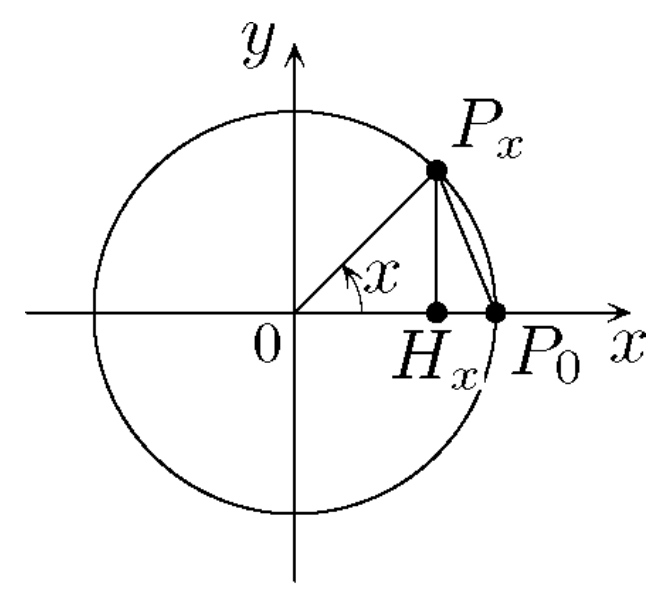
\includegraphics[width = 8cm]{inequality.png}
        \caption{Связь синуса и его аргумента}
    \end{figure}
    Всё доказано. $\blacksquare$

    \textbf{Теорема}: функции $\sin{x}$, $\cos{x}$, $\tg x$, $\ctg x$ непрерывны каждая на своей
    области определения.
    $\square$ В силу леммы:
    \begin{equation*}
        |\sin{x} - \sin{a}| = \left|2\sin{\dfrac{x - a}{2}}\cos{\dfrac{x + a}{2}}\right| \leq
        2\cdot\left|\dfrac{x - a}{2}\right|\cdot 1 = |x - a|
    \end{equation*}
    Поэтому $\forall a\in\mathbb{R}$ выполняется:
    \begin{equation*}
        \forall\varepsilon > 0\hookrightarrow\exists\delta(\varepsilon) = \varepsilon: \forall x,
        |x - a| < \delta\hookrightarrow |\sin{x} - \sin{a}| < \varepsilon.
    \end{equation*}
    Таким образом, $\sin{x}$ непрерывна в каждой точке. Непрерывность $\cos{x}$ доказывается
    аналогично. $\tg x$ и $\ctg x$ непрерывны на своих областях определения как отношения
    непрерывных функций. $\blacksquare$

    Функции $\arcsin{x}$, $\arccos{x}$, $\arctg x$, $\arcctg x$ непрерывны как обратные функции
    соответственно к $\sin{x}$, $\cos{x}$, $\tg x$, $\ctg x$ на соответствующих промежутках.

\subsection{Определение и свойства показательной функции}

    \textbf{Определение}: пусть $a > 1$, $x\in\mathbb{R}$, тогда значение $a^x$ определяется как
    $\lim\limits_{n\to\infty} a^{r_n}$, где $r_n$ -- произвольная последовательность рациональных
    чисел такая, что $\lim\limits_{n\to\infty} r_n = x$.

    Установим корректность этого определения:

    $\square$ I) \textit{Существование}:

    Предварительно докажем, что $\forall a > 0\hookrightarrow \lim\limits_{n\to\infty} \sqrt[n]{a} =
    \lim\limits_{n\to\infty} a^{\frac{1}{n}} = 1$.

    Если $a > 1$, то в силу того, что $\sqrt[n]{a} > 1$, выполняется $\sqrt[n]{a} = 1 + \beta_n$,
    где $\beta_n > 0$. Тогда:
    \begin{equation*}
        a = (1 + \beta_n)^n \geq 1 + n\beta_n > n\beta_n \implies 0 < \beta_n < \dfrac{a}{n}.
    \end{equation*}
    По теореме о двух милиционерах, $\lim\limits_{n\to\infty} \beta_n = 0 \implies
    \lim\limits_{n\to\infty} \sqrt[n]{a} = 1$.

    Если $0 < a < 1$, то $b = \dfrac{1}{a} > 1$. Тогда из предыдущего предела следует, что
    \begin{equation*}
        \lim\limits_{n\to\infty} \sqrt[n]{a} = \dfrac{1}{\lim\limits_{n\to\infty} \sqrt[n]{b}} = 1.
    \end{equation*}
    При $a = 1$ последовательность постоянна, и утверждение очевидно. Теперь перейдём к
    доказательству корректности определения.

    Так как $\lim\limits_{n\to\infty} a^{\frac{1}{n}} = 1$, то $\lim\limits_{n\to\infty}
    a^{-\frac{1}{n}} = \dfrac{1}{\lim\limits_{n\to\infty} a^{\frac{1}{n}}} = 1$. Значит:
    \begin{equation*}
        \forall\varepsilon > 0\hookrightarrow\exists k(\varepsilon)\in\mathbb{N}: -\varepsilon <
        a^{-\frac{1}{k}} - 1 < a^{\frac{1}{k}} - 1 < \varepsilon
    \end{equation*}
    (указанное неравенство выполняется при всех $k \geq k_0(\varepsilon)$, но для доказательства
    достаточно одного такого числа).

    Пусть теперь $r_n$ -- произвольная сходящаяся последовательность рациональных чисел. Докажем,
    что последовательность $y_n = a^{r_n}$ также сходится. Для произвольных $n, m\in\mathbb{N}$
    имеем:
    \begin{equation*}
        |y_n - y_m| = |a^{r_n} - a^{r_m}| = a^{r_m}|a^{r_n - r_m} - 1|
    \end{equation*}
    Так как $r_n$ сходится, то она ограничена сверху: $\exists C\in\mathbb{N}: \forall m \in
    \mathbb{N}\hookrightarrow r_m \leq C$. Значит, $a^{r_m} \leq a^C$. Так как последовательность
    $r_n$ сходится, то она фундаментальна $\implies$ для числа $k(\varepsilon)$:
    \begin{equation*}
        \exists n_0(k(\varepsilon))\in\mathbb{N}: \forall n, m \geq n_0 \hookrightarrow |r_n - r_m|
        < \dfrac{1}{k} \implies \forall n, m \geq n_0 \hookrightarrow -\dfrac{1}{k} < r_n - r_m <
        \dfrac{1}{k} \implies
    \end{equation*}
    \begin{equation*}
        \implies \forall n, m \geq n_0\hookrightarrow a^{-\frac{1}{k}} - 1 < a^{r_n - r_m} - 1 <
        a^{\frac{1}{n}} - 1
    \end{equation*}
    Отсюда следует, что $\forall n, m \geq n_0\hookrightarrow -\varepsilon < a^{r_n - r_m} - 1 <
    \varepsilon$. Окончательно имеем:
    \begin{equation*}
        \forall\varepsilon > 0\hookrightarrow \exists n_0(\varepsilon)\in\mathbb{N}: \forall n, m
        \geq n_0 \hookrightarrow a^{r_m}|a^{r_n - r_m} - 1| < a^C\cdot\varepsilon \implies \forall
        n, m \geq n_0 \hookrightarrow |y_n - y_m| < a^C\cdot\varepsilon
    \end{equation*}
    Таким образом, последовательность $y_n$ фундаментальна, следовательно, сходится.

    II) \textit{Единственность}:

    Доказано, что $\forall r_n\in\mathbb{Q}: \lim\limits_{n\to\infty} r_n = x\in\mathbb{R}
    \hookrightarrow \exists \lim\limits_{n\to\infty} a^{r_n}\in\mathbb{R}$.

    Пусть $\exists r'_n\in\mathbb{Q}, r''_n\in\mathbb{Q}: \lim\limits_{n\to\infty} r'_n =
    \lim\limits_{n\to\infty} r''_n = x$, но $\lim\limits_{n\to\infty} a^{r'_n} = y\neq z =
    \lim\limits_{n\to\infty} a^{r''_n}$.

    Рассмотрим последовательность $\gamma_n = \{r'_1, r''_1, r'_2, r''_2, ..., r'_n, r''_n, ...\}$.
    Ясно, что $\lim\limits_{n\to\infty} \gamma_n = x$ (вне любой $U_{\delta}(x)$ не более конечного
    числа членов $r'_n$ и не более конечного числа членов $r''_n$, значит, не более конечного числа
    членов $\gamma_n$). Однако последовательность $a^{\gamma_n}$ имеет два различных частичных
    предела, а значит, расходится -- противоречие.

    III) \textit{Преемственность}:

    Докажем, что если $x\in\mathbb{Q}$, то $a^x$ в смысле возведения в действительную степень
    совпадает с $a^x$ в смысле возведения в рациональную степень.

    Рассмотрим последовательность $r'_n: \forall n\in\mathbb{N}\hookrightarrow r'_n = x$, тогда
    $\lim\limits_{n\to\infty} r'_n = x$. В силу доказанной единственности, $a^x =
    \lim\limits_{n\to\infty} a^{r'_n} = a^{r'_n}$. $\blacksquare$

    При $a = 1$ определим $a^x = 1, \forall x\in\mathbb{R}$. При $0 < a < 1$ определим $a^x =
    \dfrac{1}{\left(\dfrac{1}{a}\right)^x}$; это можно сделать, так как $\dfrac{1}{a} > 1$. Таким
    образом, определена функция $f(x) = a^x$, $a > 0$, $x\in\mathbb{R}$.

    \textbf{Лемма}: $\forall x\in\mathbb{R}\hookrightarrow a^x > 0$; если $a > 1$, то $a^x$ строго
    возрастает на $\mathbb{R}$; если $0 < a < 1$, то $a^x$ строго убывает на $\mathbb{R}$.

    $\square$ Докажем сначала, что если $a > 1$, то $a^x$ строго возрастает на $\mathbb{R}$.

    Пусть $x_1 < x_2$. Рассмотрим $r', r''\in\mathbb{Q}: x_1 < r' < r'' < x_2$. $\forall n\in
    \mathbb{N}$ выберем $r_n\in\mathbb{Q}: r_n\in\left(x_1; x_1 + \dfrac{1}{n}\right)$.

    По теореме о двух милиционерах: $\lim\limits_{n\to\infty} r_n = x_1$. Тогда по определению
    возведения в действительную степень: $\lim\limits_{n\to\infty} a^{r_n} = a^{x_1}$. Так как
    $x_1 < r'$, то
    \begin{equation*}
        \exists n_0\in\mathbb{N}: \forall n\geq n_0\hookrightarrow r_n < r' \implies
        \forall n\geq n_0\hookrightarrow a^{r_n} < a^{r'}
    \end{equation*}
    Тогда по теореме о переходе к пределу в
    неравенстве: $\lim\limits_{n\to\infty} a^{r_n} = a^{x_1} \leq a^{r'}$. Аналогично, $a^{r''}
    \leq a^{x_2}$. Так как $a^{r'} < a^{r''}$, то $a^{x_1} < a^{x_2}$, то есть $a^x$ строго
    возрастает на $\mathbb{R}$ при $a > 1$. По принципу Архимеда:
    \begin{equation*}
        \forall x\in\mathbb{R}\hookrightarrow\exists k\in\mathbb{N}: k > x \iff
        \exists k\in\mathbb{N}: -x > -k \implies
    \end{equation*}
    \begin{equation*}
        \implies \forall x\in\mathbb{R}\hookrightarrow\exists k\in
        \mathbb{N}: x > -k \implies a^x > a^{-k} > 0
    \end{equation*}
    Лемма доказана для $a > 1$.

    Если $0 < a < 1$, то $\dfrac{1}{a} > 1$. Значит, $\forall x\in\mathbb{R}\hookrightarrow a^x =
    \dfrac{1}{\left(\dfrac{1}{a}\right)^x} > 0$ и строго убывает на $\mathbb{R}$.

    \textbf{Теорема}: $\forall a > 0$ функция $a^x$ непрерывна на $\mathbb{R}$.

    $\square$ В силу соотношения $a^x = \dfrac{1}{\left(\dfrac{1}{a}\right)^x}$ теорему достаточно
    доказать при $a > 1$.

    Рассмотрим любую последовательность $x_n\in\mathbb{R}: \lim\limits_{n\to\infty} x_n = x_0$,
    $x_0 < x_n$. Тогда найдётся последовательность $r_n\in\mathbb{Q}: x_0 < x_n < r_n$ (достаточно
    выбрать $\forall n\in\mathbb{N}$ рациональную точку $r_n\in\left(x_n; x_n + \dfrac{1}{n}\right)$).

    Ясно, что $0 < r_n - x_0 < x_n - x_0 + \dfrac{1}{n}$. Так как $\lim\limits_{n\to\infty} x_n =
    x_0$, то $\lim\limits_{n\to\infty} (x_n - x_0) = 0$. Поэтому $\lim\limits_{n\to\infty} \left(x_n
    - x_0 + \dfrac{1}{n}\right) = 0$. По теореме о двух милиционерах: $\lim\limits_{n\to\infty} r_n
    = x_0$.

    Так как $x_0 < x_n < r_n$, то $a^{x_0} < a^{x_n} < a^{r_n}$. По определению степени с
    действительным показателем: $\lim\limits_{n\to\infty} a^{r_n} = a^{x_0}$. Тогда по теореме о
    двух милиционерах: $\lim\limits_{n\to\infty} a^{x_n} = a^{x_0}$. Так как последовательность
    $x_n$ любая, то $\lim\limits_{x\to x_0 + 0}a^x = a^x_0$. Аналогично
    $\lim\limits_{x\to x_0 - 0}a^x = a^x_0$. Таким образом, $\lim\limits_{x\to x_0}a^x = a^{x_0}$.
    Значит, $a^x$ непрерывная в любой точке $x_0\in\mathbb{R}$. $\blacksquare$

    \textbf{Лемма}: 1) $\lim\limits_{x\to +\infty} a^x = +\infty$, $\lim\limits_{x\to -\infty}
    a^x = +0$, если $a > 1$; 2) $\lim\limits_{x\to +\infty} a^x = +0$, $\lim\limits_{x\to -\infty}
    a^x = +\infty$, если $0< a < 1$.

    $\square$ В силу соотношения $a^x = \dfrac{1}{\left(\dfrac{1}{a}\right)^x}$ достаточно доказать первую
    часть леммы.

    Так как при $a > 1$ функция $a^x$ строго возрастает на $\mathbb{R}$, то по теореме о пределах
    монотонных функций: $\exists \lim\limits_{x\to +\infty} a^x$ (конечный или $+\infty$). Достаточно
    доказать, что хотя бы для одной последовательности $x_n: \lim\limits_{n\to\infty} x_n = +\infty
    \hookrightarrow \lim\limits_{n\to\infty} a^{x_n} = +\infty$. Тогда для любой другой
    последовательности это также будет верно. Рассмотрим $x_n = n$. Так как $\lim\limits_{n\to\infty}
    \left(\dfrac{1}{a}\right)^n = +0$, то $\lim\limits_{n\to\infty} a^n = +\infty$. Значит,
    $\lim\limits_{x\to +\infty} a^x = +\infty$. Аналогично при $x_n = -n$ выполняются равенства
    $\lim\limits_{n\to\infty} x_n = -\infty \implies \lim\limits_{n\to\infty} a^{x_n} =
    \lim\limits_{n\to\infty} \left(\dfrac{1}{a}\right)^n = +0 \implies \lim\limits_{x\to -\infty}
    a^x = +0$. $\blacksquare$

    \textbf{Лемма}: $\forall a, b > 0,\ \forall x, y\in\mathbb{R}$ выполняются следующие равенства:
    \begin{enumerate}
        \item $(ab)^x = a^xb^x$;
        \item $\left(\dfrac{a}{b}\right)^x = \dfrac{a^x}{b^x}$;
        \item $a^{x+y} = a^xa^y$;
        \item $(a^x)^y = a^{xy}$.
    \end{enumerate}
    $\square$ Докажем свойство 3.

    Рассмотрим любые последовательности $x_n, y_n\in\mathbb{Q}:
    \lim\limits_{n\to\infty} x_n = x, \lim\limits_{n\to\infty} y_n = y$. Тогда $a^{x_n + y_n} =
    a^{x_n}a^{y_n}$ и $\lim\limits_{n\to\infty} (x_n + y_n) = x + y$. По определению непрерывности
    по Гейне:
    \begin{equation*}
        a^{x + y} = \lim\limits_{n\to\infty} a^{x_n + y_n} = \lim\limits_{n\to\infty} a^{x_n}\cdot
        \lim\limits_{n\to\infty} a^{y_n} = a^x\cdot a^y
    \end{equation*}
    Свойства 1, 2, 4 доказываются аналогично.

    Докажем свойство 5.
    Пусть сначала $y = r\in\mathbb{Q}$. Докажем, что $\forall x\in\mathbb{R}\hookrightarrow (a^x)^r
    = a^{xr}$.

    Рассмотрим произвольную последовательность $x_n\in\mathbb{Q}: \lim\limits_{n\to\infty} x_n = x$,
    тогда $\lim\limits_{n\to\infty} x_nr = xr$. В силу непрерывности функции $a^x$:
    \begin{equation*}
        \lim\limits_{n\to\infty} a^{x_n} = a^x,\ \lim\limits_{n\to\infty} a^{x_nr} = a^{xr}.
    \end{equation*}
    Так как $a^{x_nr} = (a^{x_n})^r$, то в силу непрерывности функции $x^r$ в точке $a^x > 0$ имеем:
    \begin{equation*}
        \lim\limits_{n\to\infty} a^{x_nr} = \lim\limits_{n\to\infty} (a^{x_n})^r = (a^x)^r.
    \end{equation*}
    Пусть теперь $y\in\mathbb{R}$. Рассмотрим произвольную последовательность $r_n\in\mathbb{Q}:
    \lim\limits_{n\to\infty} r_n = y$. В силу доказанного выше соотношения имеем: $(a^x)^{r_n} =
    a^{xr_n}$.

    Так как при фиксированном $x$ функция $f(y) = (a^x)^y$ непрерывна по $y$, то
    $\lim\limits_{n\to\infty} (a^x)^{r_n} = (a^x)^y$.

    Также $\lim\limits_{n\to\infty} xr_n = xy$ и $\lim\limits_{n\to\infty} a^{xr_n} = a^{xy}$ в силу
    непрерывности функции $a^x$.

    Так как $(a^x)^{r_n} = a^{xr_n}$, то $\lim\limits_{n\to\infty} (a^x)^{r_n} =
    \lim\limits_{n\to\infty} a^{xr_n}$ $\implies$ $(a^x)^y = a^{xy}$. $\blacksquare$

\subsection{Замечательные пределы}

    \textbf{Теорема (первый замечательный предел)}:
    \begin{equation*}
        \lim\limits_{x\to 0} \dfrac{\sin{x}}{x} = 1
    \end{equation*}

    $\square$ Функция $\dfrac{\sin{x}}{x}$ определена при $x\neq 0$. Если $0 < x < \dfrac{\pi}{2}$,
    то $\sin{x} < x$.
    \begin{figure}[H]
        \centering
        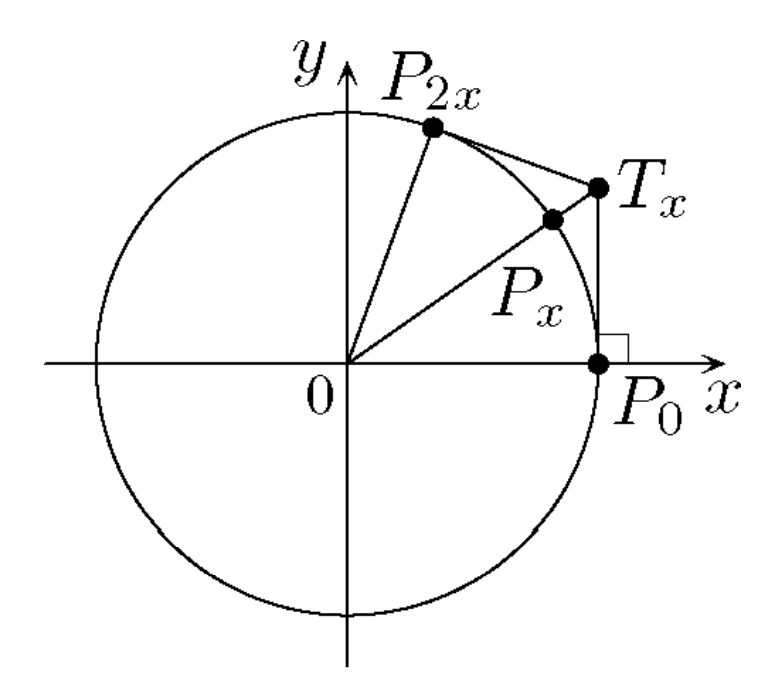
\includegraphics[width = 7.2cm]{limit.png}
        \caption{Первый замечательный предел}
    \end{figure}
    $\tg x = P_0T_x$. Далее, $P_0T_x + T_xP_{2x} > \cup P_0P_{2x}$. В силу симметрии относительно
    прямой $OP_x$, имеет место неравенство $P_0T_x > \cup P_0P_x$, то есть $\tg x > x$.

    Итак, при $0 < x < \dfrac{\pi}{2}$ имеет место неравенство:
    \begin{equation*}
        \sin{x} < x < \tg x \implies 1 < \dfrac{x}{\sin{x}} < \dfrac{1}{\cos{x}} \implies
        \cos{x} < \dfrac{\sin{x}}{x} < 1.
    \end{equation*}
    В силу чётности функций $\cos{x}$ и $\dfrac{\sin{x}}{x}$ последнее неравенство выполняется при
    $|x| < \dfrac{\pi}{2}$, $x\neq 0$, то есть в $\mathring U_{\frac{\pi}{2}}(0)$. Так как
    $\cos{x}$ непрерывна в точке $x = 0$, то $\lim\limits_{x\to 0}\cos{x} = \cos{0} = 1$.

    По теореме о двух милиционерах: $\lim\limits_{x\to 0} \dfrac{\sin{x}}{x} = 1$. $\blacksquare$

    \textbf{Теорема (второй замечательный предел)}:
    \begin{equation*}
        \lim\limits_{x\to 0} (1 + x)^{\dfrac{1}{x}} = e
    \end{equation*}

    $\square$ По определению: $e = \lim\limits_{n\to\infty} a_n$, где
    $a_n = \left(1 +\dfrac{1}{n}\right)^n$. Рассмотрим последовательность $n_k\in\mathbb{N}:
    \lim\limits_{k\to\infty} n_k = +\infty$. Вне любой $U_{\varepsilon}(e)$ содержится не более
    конечного числа членов $a_n$. Пусть $n_0(\varepsilon)$ -- наибольший из их номеров. Так как
    $\lim\limits_{k\to\infty} n_k = +\infty$, то среди членов $n_k$ лишь конечное число не
    превосходит $n_0(\varepsilon)$. Значит, вне $U_{\varepsilon}(e)$ содержится лишь конечное число
    членов $a_{n_k}$. Поэтому
    \begin{equation}\label{condition}
        \lim\limits_{k\to\infty} (1 + \dfrac{1}{n_k})^{n_k} = e
    \end{equation}
    Рассмотрим теперь последовательности $x_k\in\mathbb{R}: \lim\limits_{k\to\infty} x_k = 0$,
    $x_k > 0$ и $n_k = [\dfrac{1}{x_k}]$.

    По определению целой части числа: $\forall k\in\mathbb{N}\hookrightarrow n_k \leq \dfrac{1}{x_k}
    < n_k + 1$. Отсюда следует, что $\lim\limits_{k\to\infty} n_k = +\infty$ $\implies$ имеет место
    \eqref{condition}. Также $\dfrac{1}{n_k + 1} < x_k \leq \dfrac{1}{n_k}$. Поэтому:
    \begin{equation*}
        \left(1 + \dfrac{1}{n_k + 1}\right)^{n_k} < (1 + x_k)^{\frac{1}{x_k}} <
        \left(1 + \dfrac{1}{n_k}\right)^{n_k + 1}
    \end{equation*}
    Правая часть неравенств:
    \begin{equation*}
        \lim\limits_{k\to\infty} \left(1 + \dfrac{1}{n_k}\right)^{n_k + 1} =
        \lim\limits_{k\to\infty} \left(1 + \dfrac{1}{n_k}\right)^{n_k}\cdot
        \left(1 + \dfrac{1}{n_k}\right) = e\cdot 1 = e
    \end{equation*}
    Левая часть неравенств (следует из \eqref{condition}):
    \begin{equation*}
        \lim\limits_{k\to\infty} \left(1 + \dfrac{1}{n_k + 1}\right)^{n_k} =
        \lim\limits_{k\to\infty} \dfrac{\left(1 + \dfrac{1}{n_k + 1}\right)^{n_k + 1}}
        {1 + \dfrac{1}{n_k + 1}} = \dfrac{e}{1} = e
    \end{equation*}
    По теореме о двух милиционерах: $\lim\limits_{k\to\infty} (1 + x_k)^{\frac{1}{x_k}} = e$. Так
    как $x_k$ любая, то $\lim\limits_{x\to +0} (1 + x)^{\frac{1}{x}} = e$.

    Теперь найдём предел слева. Сначала сделаем замену $y = -x$: если $x\to -0$, то $y\to +0$, и
    $y\neq 0$ при $x\neq 0$. Имеем:
    \begin{equation*}
        \lim\limits_{x\to -0} (1 + x)^{\frac{1}{x}} = \lim\limits_{y\to +0} (1 - y)^{-\frac{1}{y}}
    \end{equation*}
    Теперь сделаем замену $z = \dfrac{y}{1 - y}$: если $y\to +0$, то $z\to +0$, и $z\neq 0$ при
    $y\neq 0$. При этом $y = \dfrac{z}{1 + z}$. Имеем:
    \begin{equation*}
        \lim\limits_{y\to +0} (1 - y)^{-\frac{1}{y}} =
        \lim\limits_{z\to +0} {\left(1 - \dfrac{z}{1 + z}\right)}^{-\frac{1+z}{z}} =
        \lim\limits_{z\to +0} \left(\dfrac{1}{1 + z}\right)^{-\left(1 + \frac{1}{z}\right)} =
    \end{equation*}
    \begin{equation*}
        = \lim\limits_{z\to +0} (1 + z)^{1 + \frac{1}{z}} =
        \lim\limits_{z\to +0} (1 + z)^{\frac{1}{z}}\cdot\lim\limits_{z\to +0} (1 + z) =
        e\cdot 1 = e
    \end{equation*}
    Таким образом, $\lim\limits_{x\to -0} (1 + x)^{\frac{1}{x}} = e$.

    Итак, $\lim\limits_{x\to +0} (1 + x)^{\frac{1}{x}} = \lim\limits_{x\to -0} (1 + x)^{\frac{1}{x}}
    = e$ $\implies$ $\lim\limits_{x\to 0} (1 + x)^{\frac{1}{x}} = e$. $\blacksquare$

    \textbf{Пример 1}:
    \begin{equation*}
        \lim\limits_{x\to 0} \dfrac{\ln{(1 + x)}}{x} = 1
    \end{equation*}

    $\square$ Так как $g(u) = \ln{(u)}$ непрерывна в точке $u = e$, то по теореме о переходе к
    пределу под знаком непрерывной функции:
    \begin{equation*}
        \lim\limits_{x\to 0} \dfrac{\ln{(1 + x)}}{x} = \lim\limits_{x\to 0}
        (\ln{(1 + x)})^{\frac{1}{x}} = \ln{\left(\lim\limits_{x\to 0} (1 + x)^{\frac{1}{x}}\right)}
        = \ln{e} = 1
    \end{equation*}
    $\blacksquare$

    \textbf{Пример 2}:
    \begin{equation*}
        \lim\limits_{x\to 0} \dfrac{e^x - 1}{x} = 1
    \end{equation*}
    $\square$ В пределе $\lim\limits_{u\to 0} \dfrac{\ln{(1 + u)}}{u} = 1$ сделаем замену
    $u = e^x - 1$: если $x\to 0$, то $u\to 0$, и $u\neq 0$ при $x\neq 0$. Предел примет вид:
    \begin{equation*}
        \lim\limits_{x\to 0} \dfrac{\ln{(1 + e^x - 1)}}{e^x - 1} = 1 \iff \lim\limits_{x\to 0}
        \dfrac{x}{e^x - 1} = 1
    \end{equation*}
    Таким образом, $\lim\limits_{x\to 0} \dfrac{e^x - 1}{x} = 1$. $\blacksquare$

\newpage
\section{БИЛЕТ 9}

\subsection{Производная функции одной переменной. Односторонние производные. Непрерывность функции,
            имеющей производную}

    \textbf{Определение}: производной функции $f(x)$ в точке $x_0$ называется предел
    \begin{equation*}
        \lim\limits_{x\to x_0} \dfrac{f(x) - f(x_0)}{x - x_0},
    \end{equation*}
    если этот предел конечен или равен $+\infty$ или $-\infty$; обозначается производная в точке
    $x_0$ как $f'(x_0)$.

    Равносильная запись предела: $\lim\limits_{\Delta x\to 0} \dfrac{f(x_0 + \Delta x) -
    f(x_0)}{\Delta x}$.

    \textbf{Определение}: правой (левой) производной функции $f(x)$ в точке $x_0$ называется предел
    \begin{equation*}
        \lim\limits_{x\to x_0 + 0} \dfrac{f(x) - f(x_0)}{x - x_0}\ \left(\text{соответственно, }
        \lim\limits_{x\to x_0 - 0} \dfrac{f(x) - f(x_0)}{x - x_0}\right),
    \end{equation*}
    если этот предел конечен или равен
    $+\infty$ или $-\infty$; обозначается правая (левая) производная в точке $x_0$ как $f'_{+}(x_0)$
    (соответственно, $f'_{-}(x_0)$).

    \textbf{Теорема}: если функция $f(x)$ имеет конечную производную (правую производную, левую
    производную) в точке $x_0$, то эта функция непрерывна (соответственно, непрерывна справа,
    непрерывна слева) в этой точке.

    $\square$ Докажем для обычной производной, для односторонних производных доказательство аналогично.
    Если $\lim\limits_{x\to x_0} \dfrac{f(x) - f(x_0)}{x - x_0} = A\in\mathbb{R}$, то $\dfrac{f(x) -
    f(x_0)}{x - x_0} = A + \alpha(x)$, где $\lim\limits_{x\to x_0} \alpha(x) = 0$.

    Тогда $f(x) = f(x_0) + (A + \alpha(x))(x - x_0) \implies \lim\limits_{x\to x_0} f(x) = f(x_0)$,
    то есть функция $f(x)$ непрерывна в точке $x_0$. $\blacksquare$

\subsection{Производная суммы, произведения, частного двух функций}

    \textbf{Теорема}: пусть функции $f(x)$ и $g(x)$ имеют конечные производные в точке $x_0$, тогда
    функции $f(x) + g(x)$, $f(x)g(x)$, $\dfrac{f(x)}{g(x)}$ имеют конечные производные в точке $x_0$
    (в последнем случае нужно требовать $g'(x_0)\neq 0$), причём в точке $x_0$ выполняются равенства:
    \begin{enumerate}
    \item $(f(x) + g(x))' = f'(x) + g'(x)$;
    \item $(f(x)g(x))' = f'(x)g(x) + f(x)g'(x)$;
    \item $\left(\dfrac{f(x)}{g(x)}\right)' = \dfrac{f'(x)g(x) - f(x)g'(x)}{g(x)^2}$.
    \end{enumerate}

    $\square$
    1)
    \begin{equation*}
        (f(x_0) + g(x_0))' = \lim\limits_{t\to 0}\dfrac{f(x_0 + t) + g(x_0 + t) - f(x_0) - g(x_0)}{t} =
    \end{equation*}
    \begin{equation*}
        = \lim\limits_{t\to 0} \dfrac{f(x_0 + t) - f(x_0)}{t} + \lim\limits_{t\to 0}
        \dfrac{g(x_0 + t) - g(x_0)}{t} = f'(x_0) + g'(x_0)
    \end{equation*}

    2)
    \begin{equation*}
        (f(x_0)g(x_0))' =
        \lim\limits_{t\to 0} \dfrac{f(x_0 + t)g(x_0 + t) - f(x_0)g(x_0)}{t} =
    \end{equation*}
    \begin{equation*}
        \lim\limits_{t\to 0} \left(\dfrac{f(x_0 + t)g(x_0 + t) - f(x_0)g(x_0 + t)}{t} +
                                   \dfrac{f(x_0)g(x_0 + t) - f(x_0)g(x_0)}{t}\right) =
    \end{equation*}
    \begin{equation*}
        = \lim\limits_{t\to 0} g(x_0 + t)\cdot\lim\limits_{t\to 0} \dfrac{f(x_0 + t) - f(x_0)}{t} +
          f(x_0)\lim\limits_{t\to 0} \dfrac{g(x_0 + t) - g(x_0)}{t} =
        f'(x_0)g(x_0) + f(x_0)g'(x_0)
    \end{equation*}
    Функция $g(x)$ имеет конечную производную в точке $x_0 \implies$ функция непрерывна в этой точке
    $\implies \lim\limits_{t\to 0}g(x_0 + t) = g(x_0)$.

    3)
    \begin{equation*}
        \left(\dfrac{f(x)}{g(x)}\right)' =
        \lim\limits_{t\to 0} \dfrac{\dfrac{f(x_0 + t)}{g(x_0 + t)} - \dfrac{f(x_0)}{g(x_0)}}{t} =
    \end{equation*}
    \begin{equation*}
        = \lim\limits_{t\to 0} \dfrac{f(x_0 + t)g(x_0) - f(x_0)g(x_0) -
                                      f(x_0)g(x_0 + t) + f(x_0)g(x_0)}{g(x_0)g(x_0 + t)t} =
    \end{equation*}
    \begin{equation*}
        \dfrac{1}{g(x_0)^2}\left(g(x_0)\lim\limits_{t\to 0}\dfrac{f(x_0 + t) - f(x_0)}{t} -
                                 f(x_0)\lim\limits_{t\to 0}\dfrac{g(x_0 + t) - g(x_0)}{t}\right) =
        \dfrac{f'(x_0)g(x_0) - f(x_0)g'(x_0)}{g(x_0)^2}\ \blacksquare
    \end{equation*}

    \textbf{Следствия}:
    \begin{enumerate}
        \item $(Cf(x))' = Cf'(x)$;
        \item $(f(x) - g(x))' = f'(x) - g'(x)$.
    \end{enumerate}

    \textit{Замечание}: данная теорема естественно переносится на односторонние пределы.

\subsection{Производная сложной функции}

    \textbf{Теорема (производная сложной функции)}: пусть функция $f(x)$ имеет конечную производную
    в точке $x_0$, а функция $g(u)$ имеет конечную производную в точке $u_0 = f(x_0)$, тогда функция
    $h(x) = g(f(x))$ имеет производную в точке $x_0$, причём $h'(x_0) = g'(u_0)f'(x_0)$.

    $\square$ Пусть $f'(x_0) = A$, $g'(u_0) = B$. Нужно доказать, что производная $h'(x_0)$
    существует и равна $AB$. По определению производной:
    \begin{equation*}
    \lim\limits_{t\to 0}\dfrac{f(x_0 + t) - f(x_0)}{t} = A,\
    \lim\limits_{s\to 0}\dfrac{g(u_0 + s) - g(u_0)}{s} = B
    \end{equation*}
    Отсюда имеем:
    \begin{equation*}
        f(x_0 + t) = f(x_0) + At + t\alpha(t)\text{, где }\lim\limits_{t\to 0}\alpha(t) = 0,
    \end{equation*}
    \begin{equation}\label{e}
        g(u_0 + s) = g(u_0) + Bs + s\beta(s),\text{ где }\lim\limits_{s\to 0}\beta(s) = 0.
    \end{equation}
    Так как $\lim\limits_{t\to 0}\alpha(t) = 0$, то $\alpha(t)$ определена в некоторой $\mathring
    U_{\delta}(0)$, но если доопределить $\alpha(0) = 0$, то $\alpha(t)$ определена в
    $U_{\delta}(0)$ и непрерывна в точке $t = 0$. Аналогично считаем, что функция $\beta(s)$
    определена в $U_{\varepsilon}(0)$ и непрерывна в точке $s = 0$, причём $\beta(0) = 0$.

    Рассмотрим функцию $s(t) = At + t\alpha(t)$. Она непрерывна в точке $t = 0$. Если равенство
    \eqref{e} выполняется $\forall s\in U_{\epsilon}(0)$, то так как $\lim\limits_{t\to 0} s(t) = 0$,
    то \eqref{e} выполняется $\forall t\in U_{\delta_1}(0)$. Значит, $\forall t\in U_{\delta_1}(0)$
    функцию $s(t)$ можно подставить в качестве $s$ в \eqref{e}. Тогда:
    \begin{equation*}
        h(x_0 + t) = g(f(x_0 + t)) = g(f(x_0) + At + t\alpha(t)) = g(u_0 + s(t)) =
    \end{equation*}
    \begin{equation*}
        = g(u_0) + Bs(t) + s(t)\beta(s(t)) = h(x_0) + ABt + Bt\alpha(t) +
        \beta(s(t))(At + t\alpha(t))
    \end{equation*}
    Таким образом:
    \begin{equation*}
        \dfrac{h(x_0 + t) - h(x_0)}{t} = AB + B\alpha(t) + \beta(s(t))(A + \alpha(t))
    \end{equation*}
    По теореме о непрерывности сложной функции:
    \begin{equation*}
        \lim\limits_{t\to 0} \beta(s(t)) = 0
    \end{equation*}
    Отсюда следует:
    \begin{equation*}
        h'(x_0) = \lim\limits_{t\to 0} \dfrac{h(x_0 + t) - h(x_0)}{t} = AB.\ \blacksquare
    \end{equation*}

\subsection{Производная обратной функции}

    \textbf{Теорема (производная  обратной функции)}: пусть функция $f(x)$ строго монотонна и
    непрерывна в некоторой $U_{\delta_0}(x_0)$, причём $\exists f'(x_0)$ (конечная, $+\infty$ или
    $-\infty$). Тогда обратная функция $g(y)$ имеет производную в точке $y_0 = f(x_0)$, причём
    $g'(y_0) = \dfrac{1}{f'(x_0)}$. Равенство формально сохраняется, если $f'(x_0) = 0$, $+\infty$
    или $-\infty$ (если $f'(x_0) = 0$ и $f(x)$ строго возрастает в $U_{\delta_0}(x_0)$, то
    $g'(y_0) = +\infty$, если $f'(x_0) = 0$ и $f(x)$ строго убывает в $U_{\delta_0}(x_0)$, то
    $g'(y_0) = -\infty$, если $f'(x_0) = +\infty$ или $-\infty$, то $g'(y_0) = 0$).

    $\square$ Пусть $I = U_{\delta_0}(x_0)$ -- промежуток. По теореме об обратной функции, на
    промежутке $J = f(I)$ определена, непрерывна и строго монотонна в ту же сторону обратная
    функция $g(y) = f^{-1}(y)$.

    Рассмотрим $x_1 = x_0 - \dfrac{\delta_0}{2}$, $x_2 = x_0 + \dfrac{\delta_0}{2}$, $x_1, x_2\in I$.
    Тогда $y_1 = f(x_1)\in J$, $y_2 = f(x_2)\in J$. Для определённости считаем, что $f(x)$ строго
    возрастает на $I$, тогда $y_1 < y_0 < y_2$, а так как $J$ -- промежуток, то $[y_1; y_2]\subset J$.
    Поэтому $\exists\varepsilon > 0: U_{\varepsilon}(y_0)\subset J$.

    Для нахождения предела:
    \begin{equation*}
        g'(y_0) = \lim\limits_{s\to 0}\dfrac{g(y_0 + s) - g(y_0)}{s}
    \end{equation*}
    сделаем замену $s(t) = f(x_0 + t) - f(x_0)$, так как в силу непрерывности функции $f(x)$ в точке
    $x_0$ имеет место равенство $\lim\limits_{t\to 0} s(t) = 0$, а также в силу строгой монотонности
    $s(t)\neq 0$ при $t\neq 0$.

    Далее:
    \begin{equation*}
        g(y_0) = x_0
    \end{equation*}
    \begin{equation*}
        g(y_0 + s) = g(f(x_0) +  f(x_0 + t) - f(x_0)) = g(f(x_0 + t)) = x_0 + t
    \end{equation*}
    Таким образом, $g(x_0 + s) - g(x_0) = t$. Поэтому:
    \begin{equation*}
        g'(y_0) = \lim\limits_{t\to 0} \dfrac{t}{f(x_0 + t) - f(x_0)} = \dfrac{1}{f'(x_0)}
    \end{equation*}
    Если $f'(x_0) = 0$ и $f(x)$ строго возрастает на $I$, то $sign(f(x_0 + t) - f(x_0)) = sign(t)$,
    дробь под знаком последнего предела положительна, и $g'(y_0) = +\infty$. Аналогично разбирается
    случай убывания $f(x)$. Если $f'(x_0) = +\infty$ или $-\infty$, то из предела видно, что
    $g'(y_0) = 0$. $\blacksquare$

    \textit{Замечание}: теорема о производной обратной функции вместе с доказательством сохраняется
    для односторонних окрестностей (у функции и обратной функции односторонние производные).

\subsection{Производные элементарных функций}

    \textbf{Производная экспоненты}: $a > 0, \forall x\in\mathbb{R}:$
    \begin{equation*}
        (a^x)' = a^x\ln{a}
    \end{equation*}

    $\square$ $(a^{x_0})' = \lim\limits_{t\to 0}\dfrac{a^{x_0 + t} - a^{x_0}}{t} =
    a^{x_0}\cdot\lim\limits_{t\to 0}\dfrac{a^t - 1}{t} = a^{x_0}\ln{a}$ $\blacksquare$

    \textbf{Производная логарифма}: $a > 0, a\neq 0, \forall x > 0:$
    \begin{equation*}
        (\log_{a}(x))' = \dfrac{1}{x\ln{a}}
    \end{equation*}

    $\square$
    \begin{equation*}
        (\log_{a}(x_0))' =
        \lim\limits_{t\to 0}\dfrac{\log_{a}(x_0 + t) - \log_{a}(x_0)}{t} =
        \lim\limits_{t\to 0}\dfrac{\log_{a}\left(1 + \dfrac{t}{x_0}\right)}{t} =
        \lim\limits_{t\to 0}\dfrac{\ln\left(1 + \dfrac{t}{x_0}\right)}{t\ln{a}} =
        \dfrac{1}{x_0\ln{a}}
    \end{equation*}
    $\blacksquare$

    \textbf{Производная степенной функции}:

    1) $\alpha\in\mathbb{R}, \forall x > 0:$
    \begin{equation*}
        (x^{\alpha})' = \alpha x^{\alpha - 1}
    \end{equation*}

    $\square$ $(x^{\alpha})' = (e^{\alpha\ln{x}})' = e^{\alpha\ln{x}}(\alpha\ln{x})' =
    x^{\alpha}\cdot\alpha\dfrac{1}{x} = \alpha x^{\alpha - 1}\ \blacksquare$

    2) $n\in\mathbb{N}, \forall x\in\mathbb{R}:$
    \begin{equation*}
        (x^n)' = nx^{n - 1}
    \end{equation*}

    $\square$ Докажем по индукции. При $n = 1$: $(x^1)' = 1\cdot x^0 = 1$ -- верно. Пусть при
    некотором $k\in\mathbb{N}$ имеет место равенство $(x^k)' = kx^{k - 1}$. Тогда $(x^{k + 1})' =
    (x^k\cdot x)' =  kx^{k - 1}\cdot x + x^k\cdot 1 = kx^k + x^k = (k+1)x^k$

    Нужное равенство получено при $n = k + 1$, значит, при $\alpha\in\mathbb{N}$ утверждение
    доказано. $\blacksquare$

    3) $m\in\mathbb{Z}, \forall x\neq 0:$
    \begin{equation*}
        (x^m)' = mx^{m - 1}
    \end{equation*}

    $\square$ Если $m = 0$, то $(x^0)' = 1' = 0$ -- верно при $x\neq 0$.

    Если $m > 0$, то $m\in\mathbb{N}$ -- уже доказано.

    Если $m < 0$, то $m = -n, n\in\mathbb{N}$. Тогда
    \begin{equation*}
        (x^{-n})' = \left(\dfrac{1}{x^n}\right)' = \dfrac{0\cdot x^n - 1\cdot nx^{n - 1}}{x^{2n}} =
        -nx^{-n-1} = mx^{m - 1}
    \end{equation*}
    Всё доказано. $\blacksquare$

    \textbf{Производная тригонометрических функций}:

    1) $\forall x\in\mathbb{R}:$
    \begin{equation*}
        (\sin{x})' = \cos{x}
    \end{equation*}

    $\square$
    \begin{equation*}
        (\sin{x_0})' = \lim\limits_{t\to 0}\dfrac{\sin(x_0 + t) - \sin(x_0)}{t} =
        \lim\limits_{t\to 0}\dfrac{2\cos\left(x_0 + \dfrac{t}{2}\right)\sin{\dfrac{t}{2}}}{t}
        \lim\limits_{t\to 0}\cos\left(x_0 + \dfrac{t}{2}\right)
        \lim\limits_{t\to 0}\dfrac{\sin{\dfrac{t}{2}}}{\dfrac{t}{2}} = \cos{x_0}
    \end{equation*}
    $\blacksquare$

    \begin{equation*}
        (\cos{x})' = -\sin{x}
    \end{equation*}
    $\square$ Доказывается аналогично. $\blacksquare$

    2) $\forall x\neq \dfrac{\pi}{2} + \pi k$, $k\in\mathbb{Z}:$
    \begin{equation*}
        (\tg x)' = \dfrac{1}{\cos^2{x}}
    \end{equation*}

    $\square$ $(\tg x)' = \left(\dfrac{\sin{x}}{\cos{x}}\right)' =
    \dfrac{\cos{x}\cos{x} - \sin{x}(-\sin{x})}{\cos^2{x}} = \dfrac{1}{\cos^2{x}}$ $\blacksquare$

    3) $\forall x\neq \pi k$, $k\in\mathbb{Z}$
    \begin{equation*}
        (\ctg x)' = -\dfrac{1}{\sin^2{x}}
    \end{equation*}
    $\square$ Доказывается аналогично. $\blacksquare$

    \textbf{Производная гиперболических функций}: $\forall x\in\mathbb{R}$ (доказывается элементарно)

    \begin{equation*}
        (\sh x)' = \ch x
    \end{equation*}
    \begin{equation*}
        (\ch x)' = \sh x
    \end{equation*}
    \begin{equation*}
        (\th x)' = \dfrac{1}{\ch^2 x}
    \end{equation*}
    \begin{equation*}
        (\cth x)' = -\dfrac{1}{\sh^2 x}
    \end{equation*}

    \textbf{Производная обратных тригонометрических функций}:

    1) В каждой точке $x\in(-1; 1)$ имеют место равенства:
    \begin{equation*}
        (\arcsin x)' = \dfrac{1}{\sqrt{1 - x^2}}
    \end{equation*}
    \begin{equation*}
        (\arccos x)' = -\dfrac{1}{\sqrt{1 - x^2}}
    \end{equation*}
    в точках $x = -1$, $x = 1$ имеют место равенства:
    \begin{equation*}
        (\arcsin{x})'|_{x = 1} = +\infty
    \end{equation*}
    \begin{equation*}
        (\arcsin{x})'|_{x = -1} = +\infty
    \end{equation*}
    \begin{equation*}
        (\arccos{x})'|_{x = 1} = -\infty
    \end{equation*}
    \begin{equation*}
        (\arccos{x})'|_{x = -1} = -\infty
    \end{equation*}

    2) В каждой точке $x\in\mathbb{R}$ имеют место равенства:
    \begin{equation*}
        (\arctg x)' = \dfrac{1}{1 + x^2}
    \end{equation*}
    \begin{equation*}
        (\arcctg x)' = -\dfrac{1}{1 + x^2}
    \end{equation*}

    $\square$ 1) Рассмотрим функцию $f(x) = \sin{x}$. Функция строго возрастает на
    $\left[-\dfrac{\pi}{2}; \dfrac{\pi}{2}\right]$; обратная функция $g(y) = f^{-1}(y) = \arcsin{y}$. В любой
    точке $y_0\in(-1; 1)$ выполняется:
    \begin{equation*}
        g'(y_0) = \dfrac{1}{f'(x_0)} = \dfrac{1}{\cos{x_0}} = \dfrac{1}{\sqrt{1 - \sin^2{x_0}}} =
        \dfrac{1}{\sqrt{1 - {y_0}^2}}
    \end{equation*}
    Здесь учтено, что $\forall x\in\left(-\dfrac{\pi}{2}; \dfrac{\pi}{2}\right)\hookrightarrow
    \cos{x} > 0$. Таким образом, $\forall x\in(-1; 1)\hookrightarrow (\arcsin{x})' =
    \dfrac{1}{\sqrt{1 - x^2}}$, равенство формально сохраняется для односторонних производных в
    точках $x = -1$ и $x = 1$.

    Формула для производной функции $\arccos{x}$ доказывается аналогично.

    2) Рассмотрим функцию $f(x) = \tg{x}$. Функция строго возрастает на $\left(-\dfrac{\pi}{2};
    \dfrac{\pi}{2}\right)$; обратная функция $g(y) = f^{-1}(y) = \arctg{y}$. В любой точке
    $y_0\in\mathbb{R}$ выполняется:
    \begin{equation*}
        g'(y_0) = \dfrac{1}{f'(x_0)} = \cos^2{x_0} = \dfrac{1}{1 + \tg^2{x_0}} =
        \dfrac{1}{1 + {y_0}^2}
    \end{equation*}
    Таким образом, $\forall x\in\mathbb{R}\hookrightarrow (\arctg{x})' = \dfrac{1}{1 + x^2}$.

    Формула для производной функции $\arcctg{x}$ доказывается аналогично. $\blacksquare$

\subsection{Дифференцируемость функции в точке, дифференциал}

    \textbf{Определение}: функция $f(x)$, определённая в некоторой окрестности точки $x_0$,
    называется дифференцируемой в этой точке, если её приращение в этой точке может быть представлено
    в виде:
    \begin{equation*}
        \Delta f(x_0) \equiv f(x_0 + \Delta x) - f(x_0) = A\cdot\Delta x + \alpha(\Delta x)\cdot
        \Delta x,\ A\in\mathbb{R},
    \end{equation*}
    где $\lim\limits_{\Delta x\to 0} \alpha(\Delta x) = 0$, то есть:
    \begin{equation*}
        \Delta f(x_0) = A\cdot\Delta x + o(\Delta x),\ \Delta x\to 0
    \end{equation*}
    При этом линейная часть приращения $A\cdot\Delta x$ называется дифференциалом функции $f(x)$ в
    точке $x_0$ и обозначается $df(x_0)$.

    \textbf{Теорема}: функция $f(x)$ дифференцируема в точке $x_0$ $\iff$ $\exists
    f'(x_0)\in\mathbb{R}$, при этом в случае дифференцируемости $A = f'(x_0)$.

    $\square$ $\boxed{\Rightarrow}$ Если $f(x_0 + \Delta x) - f(x_0) = A\cdot\Delta x +
    \alpha(\Delta x)\cdot\Delta x$, то
    \begin{equation*}
        \dfrac{f(x_0 + \Delta x) - f(x_0)}{\Delta x} = A + \alpha(\Delta x) \implies
        \lim\limits_{\Delta x\to 0} \dfrac{f(x_0 + \Delta x) - f(x_0)}{\Delta x} = A\in\mathbb{R},
    \end{equation*}
    так как $\lim\limits_{\Delta x\to 0} \alpha(\Delta x) = 0$. Таким образом, $\exists f'(x_0) =
    A\in\mathbb{R}$.

    $\boxed{\Leftarrow}$ Пусть $\lim\limits_{\Delta x\to 0} \dfrac{f(x_0 + \Delta x) -
    f(x_0)}{\Delta x} = A\in\mathbb{R}$, тогда
    \begin{equation*}
        \dfrac{f(x_0 + \Delta x) - f(x_0)}{\Delta x} = A + \alpha(\Delta x),
    \end{equation*}
    где $\lim\limits_{\Delta x\to 0} \alpha(\Delta x) = 0$. Поэтому $\Delta f(x_0) = A\cdot\Delta x
    + o(\Delta x), \Delta x\to 0$. $\blacksquare$

    \textbf{Теорема}: пусть $u = u(x), v = v(x)$ дифференцируемы в точке $x_0$, тогда имеют место
    равенства:
    \begin{enumerate}
        \item $d(u + v) = du + dv$;
        \item $d(uv) = vdu + udv$;
        \item $d\left(\dfrac{u}{v}\right) = \dfrac{vdu - udv}{v^2}$
    \end{enumerate}
    В последнем выражении $v(x_0)\neq 0$.

    $\square$ Доказывается умножением соответствующих выражений для производных на $dx$.
    $\blacksquare$

    \textbf{Теорема (инвариантность формы первого дифференциала относительно замены переменной)}: в
    равенстве $df(x) = f'(x)dx$, где $x$ -- независимая переменная, вместо $x$ можно подставить любую
    дифференцируемую функцию $u(x)$.

    $\square$ Пусть $u(x)$ дифференцируема в точке $x_0$, а функция $f(u)$ дифференцируема в точке
    $u_0 = u(x_0)$. Тогда:
    \begin{equation*}
        f'(u(x))|_{x = x_0} = f'(u_0)u'(x_0).
    \end{equation*}
    Умножим это равенство на $dx$:
    \begin{equation*}
        df(u(x)) = f'(u_0)u'(x_0)dx = f'(u_0)du.
    \end{equation*}
    То есть:
    \begin{equation*}
        df(u) = f'(u)du
    \end{equation*}
    Всё доказано. $\blacksquare$

    \subsection{Геометрический смысл производной}
    \textbf{Определение}: пусть $k(x)$ -- угловой коэффициент хорды (секущей) графика функции $f(x)$,
    проходящей через точки $M_0(x_0; y_0)$ и $M(x; y)$, где $x\neq x_0$. Если $\exists
    k = \lim\limits_{x\to x_0} k(x) = \lim\limits_{x\to x_0} \dfrac{f(x) - f(x_0)}{x - x_0}\in
    \mathbb{R}\cup\{+\infty\}\cup\{-\infty\}$, то прямая с угловым коэффициентом $k$, проходящая
    через точку $M_0$, называется касательной к графику в точке $M_0$.

    \textbf{Уравнение невертикальной касательной}:
    \begin{equation*}
        y = y_0 + f'(x_0)(x - x_0)
    \end{equation*}

\subsection{Функции, заданные параметрически, их дифференцирование}

    \textbf{Определение}: пусть $x = x(t)$ и $y = y(t)$, где $t\in I$ ($I$ - некоторый промежуток)
    тогда множество точек плоскости $\Gamma = \{(x, y): x = x(t), y = y(t), t\in I\}$ называется
    кривой (параметрически заданной) на плоскости. Если $x(t)$ и $y(t)$ непрерывны на $I$, то кривая
    $\Gamma$ называется непрерывной.

    \textbf{Теорема о локальном представлении параметрически заданной кривой}: пусть функции
    $x = x(t)$ и $y = y(t)$ непрерывны в $U_{\delta}(t_0)$, причём функция $x(t)$ строго монотонна в
    этой окрестности, тогда кривая $\Gamma = \{(x, y): x = x(t), y = y(t), t\in U_{\delta}(t_0)\}$
    является графиком непрерывной функции $y = f(x)$. Если при этом $\exists x'(t_0)\in\mathbb{R}$ и
    $\exists y'(t_0)\in\mathbb{R}$, причём $x'(t_0)\neq 0$, то $\exists f'(x_0) =
    \dfrac{y'(t_0)}{x'(t_0)}$ $\left(\text{иными словами }y'_x = \dfrac{y'_t}{x'_t}\right)$.

    $\square$ Так как функция $x(t)$ непрерывна и строго монотонна на $I = U_{\delta}(t_0)$, то по
    теореме об обратной функции на промежутке $J = x(I)$ определена и непрерывна обратная функция
    $t = t(x)$. Поэтому $(x, y)\in\Gamma \iff y = y(t(x))$, где $x\in J$, то есть кривая является
    графиком функции $y = f(x)$ на промежутке $J$. Функция $y = f(x)$ непрерывна как суперпозиция
    непрерывных функций $y(t)$ и $t(x)$. Далее, по теореме о производной обратной функции в точке
    $x_0 = x(t_0)$: $\exists t'(x_0) = \dfrac{1}{x'(t_0)}$, и по теореме о производной сложной
    функции: $\exists f'(x_0) = y'(t_0)t'(x_0) = \dfrac{y'(t_0)}{x'(t_0)}$. $\blacksquare$

\newpage
\section{БИЛЕТ 10}

\subsection{Производные высших порядков}

    \textbf{Определение}: производная порядка $n\in\mathbb{N}$ функции $f(x)$ в точке $x_0$ задаётся
    рекуррентным соотношением:
    \begin{equation*}
        f^{(n)} = \left(f^{(n - 1)}\right)',
    \end{equation*}
    где $f^{(0)} = f$, при условии, что $f^{(n - 1)}$ определена и конечна в некоторой окрестности
    точки $x_0$.

    \textbf{Свойство производной высших порядков}:
    \begin{equation*}
        \left(f^{(n)}\right)^{(m)} = f^{(n + m)}
    \end{equation*}

    \textbf{Производные порядка $n$ некоторых элементарных функций} (всё доказывается по индукции):
    \begin{equation*}
        (a^x)^{(n)} = a^x(\ln{a})^n,\ n\in\mathbb{N}_0
    \end{equation*}
    \begin{equation*}
        (x^{\alpha})^{(n)} = \alpha(\alpha - 1)...(\alpha -n + 1)x^{\alpha - n} =
        n!C_{\alpha}^{n}x^{\alpha - n},\ n\in\mathbb{N}_0
    \end{equation*}
    \begin{equation*}
        \left(\dfrac{1}{x}\right)^{(n)} = \dfrac{(-1)^nn!}{x^{n + 1}},\ n\in\mathbb{N}_0
    \end{equation*}
    \begin{equation*}
        (\ln{x})^{(n)} = \left(\dfrac{1}{x}\right)^{(n - 1)} =
        \dfrac{(-1)^{n - 1}(n - 1)!}{x^n},\ n\in\mathbb{N}
    \end{equation*}
    \begin{equation*}
        (\sin{x})^{(n)} = \sin{\left(x + \dfrac{\pi n}{2}\right)},\ n\in\mathbb{N}_0
    \end{equation*}
    \begin{equation*}
        (\cos{x})^{(n)} = \cos{\left(x + \dfrac{\pi n}{2}\right)},\ n\in\mathbb{N}_0
    \end{equation*}

    \textbf{Производная порядка $n$ от сложной функции} (всё доказывается по индукции):
    \begin{equation*}
        (f(x) + g(x))^{(n)} = f^{(n)}(x) + g^{(n)}(x)
    \end{equation*}
    \begin{equation*}
        (f(kx + b))^{(n)} = k^n\cdot f^{(n)}(kx + b)
    \end{equation*}

\subsection{Формула Лейбница для производной порядка $n$ произведения}

    \textbf{Теорема (формула Лейбница)}: пусть при $n\in\mathbb{N}$ в точке $x_0$ $\exists
    u^{(n)}(x_0)$, $\exists v^{(n)}(x_0)$, тогда произведение $u(x)v(x)$ имеет в точке $x_0$
    производную порядка $n$, причём в этой точке
    \begin{equation*}
        (uv)^{(n)} = \sum\limits_{k = 0}^n C_{n}^{k}u^{(n - k)}v^{(k)}.
    \end{equation*}

    $\square$ Доказательство проведём по индукции. При $n = 1$ имеем известную формулу
    $(uv)' = u'v + uv'$. Пусть формула Лейбница верна при некотором $n\in\mathbb{N}$. Докажем, что
    формула верна и при $n + 1$:
    \begin{equation*}
        (uv)^{(n + 1)} = \left((uv)^{(n)}\right)' =
        \left(\sum\limits_{k = 0}^n C_{n}^{k}u^{(n - k)}v^{(k)}\right)' =
        \sum\limits_{k = 0}^n C_{n}^{k}\left(u^{(n - k)}v^{(k)}\right)' =
    \end{equation*}
    \begin{equation*}
        = \sum\limits_{k = 0}^n C_{n}^{k}u^{(n - k + 1)}v^{(k)} +
          \sum\limits_{k = 0}^n C_{n}^{k}u^{(n - k)}v^{(k + 1)} =
          \sum\limits_{k = 0}^n C_{n}^{k}u^{(n - k + 1)}v^{(k)} +
          \sum\limits_{k = 1}^{n + 1} C_{n}^{k - 1}u^{(n - k + 1)}v^{(k)} =
    \end{equation*}
    \begin{equation*}
        = C_{n}^{0}u^{(n + 1)}v +
          \sum\limits_{k = 1}^n (C_{n}^{k} + C_{n}^{k - 1})u^{(n - k + 1)}v^{(k)} +
          C_{n}^{n}uv^{(n + 1)} =
    \end{equation*}
    \begin{equation*}
        = C_{n + 1}^{0}u^{(n + 1)}v + \sum\limits_{k = 1}^n C_{n + 1}^{k}u^{(n - k + 1)}v^{(k)} +
          C_{n + 1}^{n + 1}uv^{(n + 1)} =
    \end{equation*}
    \begin{equation*}
        = \sum\limits_{k = 0}^{n + 1} C_{n + 1}^{k}u^{(n + 1 - k)}v^{(k)} = (uv)^{(n + 1)}
    \end{equation*}
    Нужное равенство получено при $n + 1$. $\forall n\in\mathbb{N}$ равенство доказано.
    $\blacksquare$

\subsection{Дифференциалы высших порядков}

    \textbf{Определение}: дифференциал порядка $n$ функции $f(x)$ в точке $x$ определяется
    рекуррентным соотношением:
    \begin{equation*}
        d^nf = d(d^{n-1}f).
    \end{equation*}
    При $n = 1: d^1f = df = f'(x)dx$ -- функция от $x$ и $dx$. Если $d^{n-1}f$ -- функция от $x$ и
    $dx$, то, считая $dx$ фиксированным, а $x$ -- переменным, $d^nf$ -- дифференциал от $d^{n-1}f$
    как функции переменной $x$.

    \textbf{Свойство дифференциала порядка $n$}: если в точке $x$ $\exists f^{(n)}(x)\in\mathbb{R}$,
    то $d^nf = f^{(n)}(x)dx^n$.

    $\square$ Докажем данное утверждение по индукции. При $n = 1$ имеем: $df(x) = f'(x)dx$ --
    известное соотношение. Пусть $d^{n - 1}f(x) = f^{(n - 1)}(x)dx^{n - 1}$, тогда $dx^{n - 1}$
    считаем постоянным, откуда получаем:
    \begin{equation*}
        d^nf(x) = d\left(f^{(n - 1)}(x) \cdot dx^{n - 1}\right) =
        dx^{n - 1} \cdot d\left(f^{(n - 1)}(x)\right) =
        dx^{n - 1} \cdot f^{(n)}(x)dx = f^{(n)}dx^{n}
    \end{equation*}
    Всё доказано. $\blacksquare$

    \textbf{Отсутствие инвариантности дифференциала второго порядка относительно замены переменной}:

    Пусть $x$ -- независимая переменная, тогда $d^2f(x) = f''(x)dx^2$. Пусть теперь $u = u(x)$ имеет
    конечную вторую производную, тогда $du$ нельзя считать постоянной величиной:
    \begin{equation*}
        d^2f(u) = d\left(df(u)\right) = d\left(f'(u)du\right) = d\left(f'(u)\right)du + f'(u)d(du)
        = f''(u)du^2 + f'(u)d^2u
    \end{equation*}
    Если $u(x)$ -- независимая переменная или линейная функция от независимой переменной, то
    $d^2u = 0$; в остальных случаях $d^2u \neq 0$. Поэтому второй дифференциал не является
    инвариантным относительно замены переменной.

\newpage
\section{БИЛЕТ 11}

\subsection{Теорема Ферма}

    \textbf{Определение}: точка $x_0$ называется точкой строгого (нестрогого) локального максимума
    функции $f(x)$, если функция определена в некоторой окрестности точки $x_0$ и выполняется:
    \begin{equation*}
        \exists\delta > 0: \forall x\in \mathring U_{\delta}(x_0)\hookrightarrow f(x) < f(x_0)\ \ \
        (f(x) \leq f(x_0)).
    \end{equation*}
    Точка $x_0$ называется точкой строгого (нестрогого) локального минимума функции $f(x)$, если
    функция определена в некоторой окрестности точки $x_0$ и выполняется:
    \begin{equation*}
        \exists\delta > 0: \forall x\in \mathring U_{\delta}(x_0)\hookrightarrow f(x) > f(x_0)\ \ \
        (f(x) \geq f(x_0)).
    \end{equation*}
    Все точки локального максимума и локального минимума называются точками локального экстремума.

    \textbf{Теорема Ферма}: если в точке локального экстремума $x_0$ функции $f(x)$ (строгого или
    нестрогого) существует производная, то она равна нулю.

    $\square$ Пусть для определённости $x_0$ -- точка локального минимума (для точки локального
    максимума доказательство аналогично). Тогда
    \begin{equation*}
        f'_{+}(x_0) = \lim\limits_{x\to x_0 + 0} \dfrac{f(x) - f(x_0)}{x - x_0} \geq 0,
    \end{equation*}
    так как $f(x) \geq f(x_0)$ при $x\in(x_0; x_0 + \delta)$.

    Аналогично $f'_{-}(x_0) \leq 0$, так как $f(x) \leq f(x_0)$ при $x\in(x_0 - \delta; x_0)$.

    Так как $f'(x_0) = f'_{+}(x_0) \geq 0$  и $f'(x_0) = f'_{-}(x_0) \leq 0$, то $f'(x_0) = 0$.
    $\blacksquare$

\subsection{Теоремы о среднем}

    \textbf{Определение}: функция $f(x)$ называется дифференцируемой на промежутке $I$, если она
    имеет конечную производную в каждой внутренней точке $I$, а в концах промежутка, если они ему
    принадлежат, -- соответствующие конечные односторонние производные.

    \textbf{Определение}: функция $f(x)$ называется дифференцируемой в широком смысле на промежутке
    $I$, если она непрерывна на $I$ и
    \begin{equation*}
        \forall x \in \text{int }I \hookrightarrow \exists f'(x)\in
        \mathbb{R}\cup\{+\infty\}\cup\{-\infty\},
    \end{equation*}
    а в концах промежутка, если они ему принадлежат, существуют односторонние производные (конечные,
    или равные $+\infty$ или $+\infty$).

    \textit{Замечание}: $\text{int }I$ (внутренность $I$) -- множество, получаемое из $I$ удалением
    концов, если они ему принадлежат.

    \textbf{Теорема Ролля}: если функция $f(x)$ непрерывна на отрезке $[a; b]$ и дифференцируема в
    широком смысле на интервале $(a; b)$, причём $f(a) = f(b)$, то
    \begin{equation*}
        \exists\xi\in(a; b): f'(\xi) = 0.
    \end{equation*}

    $\square$ По первой и второй теоремам Вейерштрасса, $f(x)$ ограничена на $[a; b]$, причём
    $m = \inf\limits_{[a; b]} f(x)$ и $M = \sup\limits_{[a; b]} f(x)$ достигаются.

    Если обе точные грани достигаются в концах отрезка, то $m = M$, так как $f(a) = f(b)$, и функция
    постоянна на $[a; b] \implies \forall x\in[a; b]\hookrightarrow f'(x) = 0$.

    Пусть теперь хотя бы одна из точных верхних граней (для определённости, M) достигается в точке
    $\xi\in(a; b)$. Тогда $\xi$ -- точка локального максимума $f(x)$ (вообще говоря, нестрогого). Так
    как функция дифференцируема в широком смысле на $(a; b)$, то
    $\exists f'(\xi)\in\mathbb{R}\cup\{+\infty\}\cup\{-\infty\}$. По теореме Ферма, $f'(\xi) = 0$.
    $\blacksquare$

    \textbf{Теорема Коши}: пусть функции $f(x)$ и $g(x)$ непрерывны на отрезке $[a; b]$, $f(x)$
    дифференцируема в широком смысле на $(a; b)$, $g(x)$ дифференцируема на $(a; b)$, причём
    $\forall x\in(a; b)\hookrightarrow g'(x)\neq 0$, тогда:
    \begin{equation*}
    \exists\xi\in(a; b):\ \dfrac{f(b) - f(a)}{g(b) - g(a)} = \dfrac{f'(\xi)}{g'(\xi)}.
    \end{equation*}

    $\square$ Рассмотрим функцию $\varphi(x) = f(x) + \lambda g(x)$, где $\lambda\in\mathbb{R}$.
    Подберём $\lambda$ так, чтобы $\varphi(a) = \varphi(b)$: $f(a) + \lambda g(a) = f(b) + \lambda
    g(b)$. Получаем:
    \begin{equation*}
        \lambda = -\dfrac{f(b) - f(a)}{g(b) - g(a)}
    \end{equation*}
    Из условия теоремы следует, что $g(b) - g(a)\neq 0$: если всё же $g(b) = g(a)$, то по теореме
    Ролля $\exists x_0\in(a; b):\ g'(x_0) = 0$, но это неверно ни для какой точки интервала $(a; b)$.

    Функция $\varphi(x)$ непрерывна на $[a; b]$ и дифференцируема в широком смысле на $(a; b)$ (так
    как $g(x)$ в всех точках интервала имеет конечную производную, а $f(x)$ во всех точках интервала
    имеет конечную или определённого знака бесконечную производную).

    При найденном $\lambda$ для $\varphi(x)$ выполнено условие теоремы Ролля $\implies
    \exists\xi\in(a; b): \varphi'(\xi) = 0$, то есть $f'(\xi) + \lambda g'(\xi) = 0$. Отсюда
    получаем:
    \begin{equation*}
        \lambda = -\dfrac{f'(\xi)}{g'(\xi)}
    \end{equation*}
    Приравнивая $\lambda$, полученные разными способами, получим:
    \begin{equation*}
        \dfrac{f(b) - f(a)}{g(b) - g(a)} = \dfrac{f'(\xi)}{g'(\xi)}.
    \end{equation*}
    Всё доказано. $\blacksquare$

    \textbf{Теорема Лагранжа}: пусть функция $f(x)$ непрерывна на отрезке $[a; b]$ и дифференцируема
    в широком смысле на интервале $(a; b)$, тогда
    \begin{equation*}
        \exists\xi\in(a; b):\ f(b) - f(a) = f'(\xi)(b - a).
    \end{equation*}

    $\square$ Применим теорему Коши при $g(x) = x$ $(g'(x) = 1 \neq 0)$:
    \begin{equation*}
        \dfrac{f(b) - f(a)}{b - a} = \dfrac{f'(\xi)}{1},
    \end{equation*}
    где $\xi\in(a; b)$. $\blacksquare$

    \textbf{Теорема}: если функция $f(x)$ непрерывна на промежутке $I$, и во всех внутренних точках
    $I$ $\exists f'(x) = 0$, то $f(x)$ постоянная на $I$.

    $\square$ Пусть $x_1 < x_2$, $x_1, x_2\in I$, тогда на отрезке $[x_1; x_2]$ функция $f(x)$
    непрерывна, а на интервале $(x_1; x_2)$ дифференцируема.

    По теореме Лагранжа: $f(x_2) - f(x_1) = f'(\xi)(x_2 - x_1)$, где $\xi\in(x_1; x_2)$. Так как
    $\forall x\in(x_1; x_2)\hookrightarrow f'(x) = 0$, то $f'(\xi) = 0$ $\implies$ $f(x_1) = f(x_2)$.

    Итак, $\forall x_1, x_2\in I\hookrightarrow f(x_1) = f(x_2) \implies$ функция $f(x)$ постоянная
    на $I$. $\blacksquare$

    \textbf{Следствие}: если функции $f(x)$ и $g(x)$ непрерывны на промежутке $I$, и во всех
    внутренних точках $I$ $\exists f'(x), g'(x)$, причём $f'(x) = g'(x)$ во всех внутренних точках
    $I$, то во всех точках $I$ имеет место равенство $f(x) = g(x) + C$, где $C$ -- постоянная.

    $\square$ Рассмотрим функцию $\varphi(x) = f(x) - g(x),\ x\in I$. Функция $\varphi(x)$
    непрерывна на $I$, и во всех внутренних точках $\exists \varphi'(x) = 0 \implies \varphi(x) = C$
    на $I$, то есть $f(x) = g(x) + C$. $\blacksquare$

\subsection{Формула Тейлора}

    \textbf{Определение}: пусть функция $f(x)$ такова, что при некотором $n\in\mathbb{N}_0
    \hookrightarrow f^{(n)}(x_0)\in\mathbb{R}$, тогда многочлен
    \begin{equation*}
        P_n(f, x) = \sum\limits_{k = 0}^{n}\dfrac{f^{(k)}(x_0)}{k!}(x - x_0)^k
    \end{equation*}
    называется многочленом Тейлора порядка $n$ функции $f(x)$ в точке $x_0$; разность $r_n(f, x) =
    f(x) - P_n(f, x)$ называется остаточным членом формулы Тейлора, а равенство
    $f(x) = P_n(f, x) + r_n(f, x)$ - формулой Тейлора для функции $f(x)$ в точке $x_0$.

    \textbf{Лемма 1}: $\forall x\in\mathbb{R}\hookrightarrow 1)\ P'_n(f, x) = P_{n - 1}(f', x),\
    2)\ r'_n(f, x) = r_{n - 1}(f', x)$ при $n\in\mathbb{N}$.

    $\square$ 1):
    \begin{equation*}
        P_n(f, x) = \sum\limits_{k = 0}^{n}\dfrac{f^{(k)}(x_0)}{k!}(x - x_0)^k
    \end{equation*}
    Таким образом:
    \begin{equation*}
        P'_n(f, x) = \sum\limits_{k = 1}^{n}\dfrac{(f')^{(k - 1)}(x_0)}{k!}k(x - x_0)^{k - 1} =
        \sum\limits_{k = 1}^{n}\dfrac{(f')^{(k - 1)}(x_0)}{(k - 1)!}(x - x_0)^{k - 1} =
        P_{n - 1}(f', x)
    \end{equation*}
    2):
    \begin{equation*}
        r'_n(f, x) = (f(x) - P_n(f, x))' = f'(x) - P'_n(f, x) =
        f'(x) - P_{n-1}(f', x) = r_{n - 1}(f', x)
    \end{equation*}
    Всё доказано. $\blacksquare$

    \textbf{Лемма 2}: $\forall k\in\mathbb{N}_0: k \leq n\hookrightarrow P_{n}^{(k)}(f, x_0) =
    f^{(k)}(x_0),\ r_{n}^{(k)}(f, x_0) = 0$.

    $\square$ Многочлен Тейлора:
    \begin{equation*}
        P_n(f, x) = \sum\limits_{j = 0}^{n}\dfrac{f^{(j)}(x_0)}{j!}(x - x_0)^j,
    \end{equation*}
    Продифференцируем данную сумму $k \leq n$ раз. Тогда для всех слагаемых с $j < k$ выполняется
    $((x - x_0)^{j})^{(k)} = 0$. Поэтому $k$-я производная многочлена имеет вид:
    \begin{equation*}
        P_{n}^{(k)}(f, x) =
        \sum\limits_{j = k}^{n}\dfrac{f^{(j)}(x_0)}{j!}j(j - 1)...(j - k + 1)(x - x_0)^{j - k} =
        \sum\limits_{j = k}^{n}C_{j}^{k}f^{(j)}(x_0)(x - x_0)^{j - k} =
    \end{equation*}
    \begin{equation*}
        = f^{(k)}(x_0) + \sum\limits_{j = k + 1}^{n}C_{j}^{k}f^{(j)}(x_0)(x - x_0)^{j - k}
    \end{equation*}
    Так как многочлен Тейлора рассматривается в точке $x = x_0$, то последняя сумма равна нулю.
    Поэтому
    \begin{equation*}
        P_{n}^{(k)}(f, x_0) = f^{(k)}(x_0)
    \end{equation*}
    Так как $r_{n}^{(k)}(f, x_0) = f^{(k)}(x_0) - P_{n}^{(k)}(f, x_0)$, то $r_{n}^{(k)}(f, x_0) = 0$.
    $\blacksquare$

    \textbf{Теорема (остаточный член формулы Тейлора в форме Пеано)}: пусть при некотором
    $n\in\mathbb{N}\hookrightarrow\exists f^{(n)}(x_0)\in\mathbb{R}$, тогда остаточный член формулы
    Тейлора имеет вид:
    \begin{equation*}
        r_n(f, x) = o((x - x_0)^n),\ x\to x_0
    \end{equation*}

    $\square$ Докажем данную теорему по индукции. При $n = 1$ утверждение верно в силу
    эквивалентности дифференцируемости в точке и существования в ней конечной производной. Пусть
    теорема верна для некоторого $n\in\mathbb{N}$. Докажем, что она верна для $n + 1$.

    Если $f(x)$ имеет $(n + 1)$-ю конечную производную в точке $x_0$, то $f'(x)$ имеет $n$-ю
    конечную производную в точке $x_0$. По предположению индукции: $r_n(f', x) = o((x - x_0)^n),\
    x\to x_0$.

    Так как $\exists f^{(n + 1)}(x_0)\in\mathbb{R}$, то $\exists\delta > 0: \forall x\in
    U_{\delta}(x_0)\hookrightarrow \exists f^{(n)}(x)\in\mathbb{R}$ $\implies$ $f(x)$
    дифференцируема в $U_{\delta}(x_0)$ по крайней мере один раз.

    Далее, $r_{n + 1}(f, x) = f(x) - P_{n + 1}(f, x)$. Каждое из слагаемых дифференцируемо в
    $U_{\delta}(x_0)$, поэтому $r_{n + 1}(f, x)$ дифференцируема в $U_{\delta}(x_0)$.

    При фиксированном значении $x\in\mathring U_{\delta}(x_0)$ применим к функции $r(x) \equiv
    r_{n + 1}(f, x)$ теорему Лагранжа на отрезке $[x_0; x]$ (или на отрезке $[x; x_0]$, смотря какое
    из двух чисел больше):
    \begin{equation*}
        r(x) - r(x_0) = r'(\xi)(x - x_0),
    \end{equation*}
    где $x_0 < \xi < x$ (или $x < \xi < x_0$). В любом случае $\xi = \xi(x)$,
    $\lim\limits_{x\to x_0} \xi(x) = x_0$, $\xi(x)\neq x_0$.

    По лемме 1: $r'(x) \equiv r'_{n + 1}(f, x) = r_{n}(f', x)$. Тогда из предположения индукции
    следует, что
    \begin{equation*}
        r'(x) = o((x - x_0)^n),\ x\to x_0 \implies \lim\limits_{x\to x_0} \dfrac{r'(x)}{(x - x_0)^n} = 0
    \end{equation*}
    По теореме о замене переменной под знаком предела:
    \begin{equation*}
        \lim\limits_{x\to x_0} \dfrac{r'(\xi(x))}{(\xi(x) - x_0)^n} = 0
    \end{equation*}
    Так как $x_0 < \xi < x$ или $x < \xi < x_0$, то $|\xi(x) - x_0| < |x - x_0|$. Теперь рассмотрим
    предел:
    \begin{equation*}
        \lim\limits_{x\to x_0} \dfrac{r'(\xi(x))}{(x - x_0)^n} =
        \lim\limits_{x\to x_0}\dfrac{r'(\xi(x))}{(\xi(x) - x_0)^n}\cdot
        \dfrac{(\xi(x) - x_0)^n}{(x - x_0)^n} = 0 \implies r'(\xi(x)) = o((x - x_0)^n)
    \end{equation*}
    Предел равен нулю как произведение бесконечно малой функции на ограниченную (числитель второй
    дроби меньше знаменателя).

    По лемме 2: $r(x_0) = 0$. Тогда вернёмся к выражению из теоремы Лагранжа:
    \begin{equation*}
        r(x) = r'(\xi)(x - x_0) = o((x - x_0)^n)(x - x_0) = o((x - x_0)^{n + 1})
    \end{equation*}
    Утверждение теоремы верно для значения $n + 1$. $\blacksquare$

    \textbf{Лемма}: пусть при некотором $n\in\mathbb{N}\hookrightarrow\exists f^{(n)}(x_0)$, тогда
    если $f(x) = Q(x) + o((x - x_0)^n)$, $x\to x_0$, где $Q(x)$ -- многочлен степени не выше $n$,
    то $Q(x) = P_n(f, x)$.

    $\square$ Опустим индекс $n$. Запишем формулу Тейлора с остаточным членом в форме Пеано для
    $f(x)$ в точке $x_0$:
    \begin{equation*}
        f(x) = P(x) + o((x - x_0)^n),\ x\to x_0
    \end{equation*}
    По условию:
    \begin{equation*}
        f(x) = Q(x) + o((x - x_0)^n),\ x\to x_0
    \end{equation*}
    Вычтем одно уравнение из другого: $P(x) - Q(x) = o((x - x_0)^n),\ x\to x_0$. Введём обозначение:
    $T(x) = P(x) - Q(x)$. Докажем, что $T(x) \equiv 0$.

    Так как $T(x) = o((x - x_0)^n),\ x\to x_0$, то
    \begin{equation*}
        \lim\limits_{x\to x_0}\dfrac{T(x)}{(x - x_0)^n} = 0
    \end{equation*}
    По теореме о замене переменной под знаком предела ($x = x_0 + t$; $x\to x_0$ при $t\to 0$;
    $x\neq x_0$ при $t\neq 0$):
    \begin{equation*}
        \lim\limits_{t\to 0}\dfrac{T(x_0 + t)}{t^n} = 0 \implies T(x_0 + t) = o(t^n),\ t \to 0
        \implies \lim\limits_{t\to 0} T(x_0 + t) = 0
    \end{equation*}
    Пусть $T(x_0 + t) = a_0 + a_1t + ... + a_nt^n$ -- многочлен степени не выше $n$. Докажем, что все
    коэффициенты этого многочлена равны нулю.

    Так как $\lim\limits_{t\to 0} T(x_0 + t) = 0$, то $a_0 = 0$. Тогда $T(x) = a_1t + ... + a_nt^n =
    o(t^n),\ t \to 0$. Поделим уравнение на $t\neq 0$: $a_1 + a_2t + ... + a_nt^{n - 1} =
    o(t^{n - 1}),\ t \to 0$. В пределе $t\to 0$ получим $a_1 = 0$ и т.д. Последовательно все
    коэффициенты многочлена равны нулю. $\blacksquare$

    \textbf{Теорема (остаточный член формулы Тейлора в форме Лагранжа)}: пусть функция $f(x)$ имеет
    $(n + 1)$-ю конечную производную в $U_{\delta}(x_0)$, $n\in\mathbb{N}_0$. Тогда
    $\forall x\in U_{\delta}(x_0)$ остаточный член формулы Тейлора имеет вид:
    \begin{equation*}
        r_n(f, x) = \dfrac{f^{(n + 1)}(\xi)}{(n + 1)!}(x - x_0)^{n + 1},
    \end{equation*}
    где $\xi\in(x_0, x)$ (или $\xi\in(x, x_0)$, смотря какое из двух чисел больше).

    $\square$ При $x = x_0$ формула имеет вид $f(x_0) = f(x_0)$ и верна $\forall\xi$. Пусть
    $x > x_0$, то есть $x\in(x_0; x_0 + \delta)$ (при $x < x_0$ доказательство аналогично).

    Рассмотрим функцию $r(x) = r_n(f, x)$. Она имеет $(n + 1)$-ю конечную производную в
    $U_{\delta}(x_0)$ (а значит, непрерывна в этой окрестности), причём в силу леммы 2:
    $r(x_0) = r'(x_0) = ... = r^{(n)}(x_0) = 0$.

    Рассмотрим также функцию $s(x) = (x - x_0)^{n + 1}$. Она имеет производные всех порядков, причём
    $s(x_0) = s'(x_0) = ... = s^{(n)}(x_0) = 0$; $\forall x\in\mathbb{R}\hookrightarrow
    s^{(n + 1)}(x) = (n + 1)!$. Также ясно, что $\forall x\neq x_0\hookrightarrow$ $s'(x)\neq 0$;
    $s''(x)\neq 0$; ...; $s^{(n)}(x)\neq 0$.

    По теореме Коши:
    \begin{equation*}
        \dfrac{r(x)}{s(x)} = \dfrac{r(x) - r(x_0)}{s(x) - s(x_0)} = \dfrac{r'(\xi_1)}{s'(\xi_1)},
    \end{equation*}
    где $\xi_1\in (x_0; x)$. Далее применим теорему Коши к функциям $r'(x)$ и $s'(x)$:
    \begin{equation*}
        \dfrac{r(x)}{s(x)} = \dfrac{r'(\xi_1) - r'(x_0)}{s'(\xi_1) - s'(x_0)} =
        \dfrac{r''(\xi_2)}{s''(\xi_2)},
    \end{equation*}
    где $\xi_2\in (x_0; \xi_1)$. Продолжим цепочку:
    \begin{equation*}
        \dfrac{r(x)}{s(x)} =
        \dfrac{r''(\xi_2) - r''(x_0)}{s''(\xi_2) - s''(x_0)} =
        \dfrac{r'''(\xi_3)}{s'''(\xi_3)} = \dfrac{r^{(4)}(\xi_4)}{s^{(4)}(\xi_4)} = ... =
        \dfrac{r^{(n)}(\xi_n)}{s^{(n)}(\xi_n)} =
        \dfrac{r^{(n)}(\xi_n) - r^{(n)}(x_0)}{s^{(n)}(\xi_n) - s^{(n)}(x_0)} =
        \dfrac{r^{(n + 1)}(\xi)}{s^{(n + 1)}(\xi)},
    \end{equation*}
    где $x_0 < \xi < \xi_n < ... < \xi_2 < \xi_1 < x$, то есть $\xi\in(x_0; x)$.

    Так как $P_n(f, x)$ -- многочлен степени не выше $n$, то $P_{n}^{(n + 1)} = 0 \implies
    r^{(n + 1)}(\xi)  = f^{(n + 1)}(\xi)$. Тогда получим:
    \begin{equation*}
        r(x) = \dfrac{r^{(n + 1)}(\xi)}{s^{(n + 1)}(\xi)}s(x) =
        \dfrac{f^{(n + 1)}(\xi)}{(n + 1)!}(x - x_0)^{n + 1}
    \end{equation*}
    Всё доказано. $\blacksquare$

\subsection{Основные разложения по формуле Тейлора}

    \begin{equation*}
        e^x = \sum\limits_{k = 0}^{n} \dfrac{x^k}{k!} + o(x^n),\ x\to 0
    \end{equation*}
    \begin{equation*}
        \sh x = \sum\limits_{k = 0}^{n} \dfrac{x^{2k + 1}}{(2k + 1)!} + o(x^{2n + 2}),\ x\to 0
    \end{equation*}
    \begin{equation*}
        \ch x = \sum\limits_{k = 0}^{n} \dfrac{x^{2k}}{(2k)!} + o(x^{2n + 1}),\ x\to 0
    \end{equation*}
    \begin{equation*}
        \sin x = \sum\limits_{k = 0}^{n} \dfrac{(-1)^kx^{2k + 1}}{(2k + 1)!} + o(x^{2n + 2}),\ x\to 0
    \end{equation*}
    \begin{equation*}
        \cos x = \sum\limits_{k = 0}^{n} \dfrac{(-1)^kx^{2k}}{(2k)!} + o(x^{2n + 1}),\ x\to 0
    \end{equation*}
    \begin{equation*}
        \ln (1 + x) = \sum\limits_{k = 1}^{n} \dfrac{(-1)^{k - 1}x^k}{k} + o(x^n),\ x\to 0
    \end{equation*}
    \begin{equation*}
        (1 + x)^{\alpha} = \sum\limits_{k = 0}^{n} C_{\alpha}^{k}x^k + o(x^n),\ x\to 0
    \end{equation*}
    \begin{equation*}
        \arctg x = \sum\limits_{k = 0}^{n} \dfrac{(-1)^kx^{2k + 1}}{2k + 1} + o(x^{2n + 2}),\ x\to 0
    \end{equation*}
    \begin{equation*}
        \arcsin x =\sum\limits_{k = 0}^{n} C_{-\frac{1}{2}}^{k}\dfrac{(-1)^kx^{2k + 1}}{2k + 1} +
        o(x^{2n + 2}),\ x\to 0
    \end{equation*}
    \begin{equation*}
        \tg x = x + \dfrac{x^3}{3} + \dfrac{2}{15}x^5 + o(x^6),\ x\to 0
    \end{equation*}
    \begin{equation*}
        \th x = x - \dfrac{x^3}{3} + \dfrac{2}{15}x^5 + o(x^6),\ x\to 0
    \end{equation*}

\subsection{Правила Лопиталя}

    \textbf{Раскрытие неопределённости $\dfrac{0}{0}$}: пусть функции $f(x)$ и $g(x)$ дифференцируемы
    в некоторой проколотой окрестности $\alpha$, где $\alpha$ -- один из 6 СПС, причём
    $\lim\limits_{x\to\alpha} f(x) = \lim\limits_{x\to\alpha} g(x) = 0$. Тогда если
    $\lim\limits_{x\to\alpha} \dfrac{f'(x)}{g'(x)} = \beta$, где $\beta$ -- один из 6 СПС, то
    $\lim\limits_{x\to\alpha} \dfrac{f(x)}{g(x)} = \beta$.

    $\square$ Поскольку $\dfrac{f'(x)}{g'(x)}$ определена в некоторой проколотой окрестности $\alpha$,
    то $g'(x)\neq 0$ в этой проколотой окрестности.

    Сначала докажем теорему для случая $\alpha = a\in\mathbb{R}$. Доопределим $f(a) = g(a) = 0$,
    тогда функции $f(x)$ и  $g(x)$ дифференцируемы в $\mathring U_{\delta}(a)$ и непрерывны в
    $U_{\delta}(a)$.

    $\forall x > a:\ g'(x)\neq 0$ по теореме Коши имеем:
    \begin{equation*}
        \dfrac{f(x)}{g(x)} = \dfrac{f(x) - f(a)}{g(x) - g(a)} = \dfrac{f'(\xi)}{g'(\xi)},
    \end{equation*}
    где $\xi = \xi(x)$. Так как $a < \xi(x) < x$, то по теореме о двух милиционерах:
    $\lim\limits_{x\to a + 0} \xi(x) = a + 0$.

    Далее по теореме о замене переменной под знаком предела:
    \begin{equation*}
        \beta = \lim\limits_{x\to a + 0} \dfrac{f'(x)}{g'(x)} =
        \lim\limits_{x\to a + 0} \dfrac{f'(\xi(x))}{g'(\xi(x))} =
        \lim\limits_{x\to a + 0} \dfrac{f(x)}{g(x)}
    \end{equation*}
    Аналогично $\lim\limits_{x\to a - 0} \dfrac{f(x)}{g(x)} = \beta$. Таким образом, для
    $\alpha = a\in\mathbb{R}$ теорема доказана.

    Для $\alpha = a + 0$ и $\alpha = a - 0$ доказывается аналогично.

    Пусть теперь $\alpha = \infty$. Так как $\lim\limits_{x\to\infty} \dfrac{f'(x)}{g'(x)} = \beta$,
    то по теореме о замене переменной под знаком предела после замены $x = \dfrac{1}{t}$ имеем:
    \begin{equation*}
        \lim\limits_{t\to 0} \dfrac{f'\left(\dfrac{1}{t}\right)}{g'\left(\dfrac{1}{t}\right)} = \beta
    \end{equation*}
    Воспользуемся уже доказанным случаем $\alpha = a\in\mathbb{R}$:
    \begin{equation*}
        \lim\limits_{x\to\infty}\dfrac{f(x)}{g(x)} =
        \lim\limits_{t\to 0} \dfrac{f\left(\dfrac{1}{t}\right)}{g\left(\dfrac{1}{t}\right)} =
        \lim\limits_{t\to 0} \dfrac{\left(f\left(\dfrac{1}{t}\right)\right)'}
                                   {\left(g\left(\dfrac{1}{t}\right)\right)'} =
        \lim\limits_{t\to 0}\dfrac{f'\left(\dfrac{1}{t}\right)\cdot\left(-\dfrac{1}{t^2}\right)}
                                  {g'\left(\dfrac{1}{t}\right)\cdot\left(-\dfrac{1}{t^2}\right)} =
        \lim\limits_{t\to 0} \dfrac{f'\left(\dfrac{1}{t}\right)}{g'\left(\dfrac{1}{t}\right)} =
        \beta
    \end{equation*}
    Для $\alpha = +\infty$ и $\alpha = -\infty$ доказательство аналогично. $\blacksquare$

    \textbf{Лемма}: пусть $\lim\limits_{x\to\alpha} f(x) = \infty$, где $\alpha$ -- один из 6 СПС,
    тогда $\exists\delta > 0: \forall x\in \mathring U_{\delta}(\alpha)$ определена функция
    $\varphi(x): \lim\limits_{x\to\alpha} \varphi(x) = \alpha$, и при этом $f(\varphi(x)) = o(f(x))$,
    $x\to\alpha$.

    $\square$ Пусть сначала $\alpha = a\in\mathbb{R}$.

    Так как $\lim\limits_{x\to a} f(x) = \infty$, то $\exists\delta_1\in (0; 1): \forall x\in
    \mathring U_{\delta_1}(a)\hookrightarrow |f(x)| > 1$. При этом $f(a \pm \delta_1)\neq 0$. (Если
    последнее условие неверно для некоторой проколотой окрестности, то выбираем $\delta_1$ меньше
    изначального до тех пор, пока условие не выполнится; если оно не выполняется ни для какого
    $\delta_1$, то $\forall x\in\mathring U_{\delta}(x_0)\hookrightarrow f(x) = 0$, что неверно).

    Далее, $\exists\delta_2 > 0$, $\delta_2 < min\left(\delta_1; \dfrac{1}{2}\right): \forall
    x\in\mathring U_{\delta_2}(a)\hookrightarrow |f(x)| > |f(a \pm \delta_1)|$, то есть
    $\left|\dfrac{f(x)}{f(a \pm \delta_1)}\right| > 1$. При этом также потребуем
    $f(a \pm \delta_2)\neq 0$.

    Аналогично, $\exists\delta_3 > 0$, $\delta_3 < min\left(\delta_2; \dfrac{1}{3}\right): \forall
    x\in\mathring U_{\delta_3}(a)\hookrightarrow \left|\dfrac{f(x)}{f(a \pm \delta_2)}\right| > 2$.
    При этом также потребуем $f(a \pm \delta_3)\neq 0$.

    Таким образом, строим последовательность:
    \begin{equation*}
        \delta_n: \delta_{n + 1} < min\left(\delta_n, \dfrac{1}{n + 1}\right),\
        \forall x\in\mathring U_{\delta_{n + 1}}(a)\hookrightarrow
        \left|\dfrac{f(x)}{f(a \pm \delta_n)}\right| > n,\ f(a \pm \delta_{n + 1})\neq 0
    \end{equation*}
    Из определения последовательности $\delta_n$ ясно, что она строго убывает. Так как
    $0 < \delta_n < \dfrac{1}{n}$, то $\lim\limits_{n\to\infty} \delta_n = 0$.

    Далее, $\forall x \in \mathring U_{\delta_2}(a) \hookrightarrow \exists! n(x)\in\mathbb{N}:
    \delta_{n + 2}\leq |x - a| < \delta_{n + 1}$. Ясно, что $\forall x \in \mathring U_{\delta_2}(a)
    \hookrightarrow n(x)  > 0$. Также $n(x)$ нестрого убывает на $(a; a + \delta_2)$, нестрого
    возрастает на $(a - \delta_2; a)$. Так как $n(x)$ неограниченна на $(a - \delta_2; a)$ и на
    $(a; a + \delta_2)$, то по теореме о пределах монотонных функций:
    \begin{equation*}
        \lim\limits_{x\to a+0} n(x) = +\infty, \lim\limits_{x\to a-0} n(x) = +\infty \implies
        \lim\limits_{x\to a} n(x) = +\infty.
    \end{equation*}
    Рассмотрим функцию $\varphi(x) = a\pm \delta_{n(x)}$ (знак $+$, если $x > a$, знак $-$, если
    $x < a$). Из определения последовательности $\delta_n$ получаем:
    \begin{equation*}
        \left|\dfrac{f(\varphi(x))}{f(x)}\right| < \dfrac{1}{n(x)}
    \end{equation*}
    По теореме о переходе к пределу в неравенстве:
    \begin{equation*}
        \lim\limits_{x\to a} \left|\dfrac{f(\varphi(x))}{f(x)}\right| \leq 0
    \end{equation*}
    Поскольку $\left|\dfrac{f(\varphi(x))}{f(x)}\right| \geq 0$, то по лемме о сохранении знака:
    \begin{equation*}
        \lim\limits_{x\to a} \left|\dfrac{f(\varphi(x))}{f(x)}\right| = 0 \iff
        f(\varphi(x)) = o(f(x)),\ x\to a
    \end{equation*}
    Далее, так как $0 < \delta_{n(x)} < \dfrac{1}{n(x)}$, то по теореме о двух милиционерах:
    \begin{equation*}
        \lim\limits_{x\to a} \delta_{n(x)} = 0 \implies \lim\limits_{x\to a} \varphi(x) = a
    \end{equation*}
    Лемма доказана для случая $\alpha = a\in\mathbb{R}$. Для $\alpha = a + 0$ и $\alpha = a - 0$
    упрощения очевидны.

    Если $\alpha = \infty$, то доказательство аналогично, но $\delta_1 > 1$,
    $\delta_2 > max(\delta_1, 2)$, ..., $\delta_{n + 1} > max(\delta_n, n + 1)$. Последовательность
    $\delta_n$ строго возрастает и $\lim\limits_{n\to\infty}\delta_n = +\infty$. Неравенство с
    функцией $f(x)$ примет вид:
    \begin{equation*}
        \left|\dfrac{f(x)}{f(\pm\delta_n)}\right| > n,\ |x| > \delta_{n + 1}
    \end{equation*}
    Функция $n(x)$ определяется так: $\delta_{n + 1} < |x| \leq \delta_{n + 2}$,
    $\varphi(x) = \pm\delta_{n(x)}$ (знак $+$, если $x > 0$, знак $-$, если $x < 0$).

    Упрощения в доказательстве при $\alpha = +\infty$ и $\alpha = -\infty$ очевидны. $\blacksquare$

    \textbf{Раскрытие неопределённости $\dfrac{\infty}{\infty}$}: пусть функции $f(x)$ и $g(x)$
    дифференцируемы в некоторой проколотой окрестности $\alpha$, где $\alpha$ -- один из 6 СПС,
    причём $\lim\limits_{x\to\alpha} f(x) = \lim\limits_{x\to\alpha} g(x) = \infty$. Тогда если
    $\lim\limits_{x\to\alpha} \dfrac{f'(x)}{g'(x)} = \beta$, где $\beta$ -- один из 6 СПС, то
    $\lim\limits_{x\to\alpha} \dfrac{f(x)}{g(x)} = \beta$.

    $\square$ Определим $\varphi(x)$ как в лемме.
    Функция $\dfrac{f'(x)}{g'(x)}$ определена в некоторой проколотой окрестности $\alpha
    \implies g'(x)\neq 0$ в этой проколотой окрестности. Применим к функциям $f(x)$ и $g(x)$ теорему
    Коши на отрезке $[\varphi(x); x]$ (или на $[x; \varphi(x)]$, смотря какое из чисел больше):
    \begin{equation*}
        \dfrac{f(x) - f(\varphi(x))}{g(x) - g(\varphi(x))} =
        \dfrac{f'(\xi)}{g'(\xi)},\>\>\varphi(x) < \xi(x) < x
    \end{equation*}
    Так как $\lim\limits_{x\to\alpha}\varphi(x) = \alpha$, то по теореме о двух милиционерах:
    $\lim\limits_{x\to\alpha}\xi(x) = \alpha$.

    По теореме о замене переменной под знаком предела:
    \begin{equation*}
        \beta =
        \lim\limits_{x\to\alpha}\dfrac{f'(x)}{g'(x)} =
        \lim\limits_{x\to\alpha}\dfrac{f'(\xi(x))}{g'(\xi(x))} =
        \lim\limits_{x\to\alpha} \dfrac{f(x) - f(\varphi(x))}{g(x) - g(\varphi(x))}
    \end{equation*}
    Так как $f(\varphi(x)) = o(f(x))$ при $x\to\alpha$, то $f(x) - f(\varphi(x)) \sim f(x)$ при
    $x\to\alpha$. Аналогично, $g(x) - g(\varphi(x)) \sim g(x)$ при $x\to\alpha$. Тогда по теореме о
    замене числителя и знаменателя на эквивалентные величины при вычислении предела:
    \begin{equation*}
        \beta =
        \lim\limits_{x\to\alpha} \dfrac{f(x) - f(\varphi(x))}{g(x) - g(\varphi(x))} =
        \lim\limits_{x\to\alpha} \dfrac{f(x)}{g(x)}
    \end{equation*}
    Всё доказано. $\blacksquare$

\newpage
\section{БИЛЕТ 12}

    \textbf{Необходимые условия монотонности}: пусть функция $f(x)$ дифференцируема на интервале
    $(a; b)$, конечном или бесконечном, тогда если $f(x)$ возрастает на $(a; b)$, то $f'(x)\geq 0$
    на $(a; b)$; если убывает, то $f'(x)\leq 0$ на $(a; b)$ (монотонность, вообще говоря, нестрогая).

    $\square$ Пусть функция $f(x)$ возрастает на $(a; b)$, тогда в произвольной точке $x_0\in(a; b)$
    выполняется:
    \begin{equation*}
        f'_{+}(x_0) = \lim\limits_{t\to +0} \dfrac{f(x_0 + t) - f(x_0)}{t} \geq 0,
    \end{equation*}
    так как $f(x_0 + t) - f(x_0) > 0$ при $t > 0$. Значит, $f'(x_0) = f'_{+}(x_0) \geq 0$.

    Если $f(x)$ убывает на $(a; b)$, то доказательство аналогично. $\blacksquare$

    \textbf{Достаточные условия монотонности}: пусть функция $f(x)$ непрерывна на промежутке $I$ и
    дифференцируема во всех внутренних точках $I$. Тогда:
    \begin{enumerate}
        \item если $f'(x) > 0$ ($f'(x) < 0$) во всех внутренних точках $I$, то функция $f(x)$ строго
              возрастает (убывает) на $I$.
        \item если $f'(x) \geq 0$ ($f'(x) \leq 0$) во всех внутренних точках $I$, то функция $f(x)$
              нестрого возрастает (убывает) на $I$.
    \end{enumerate}

    $\square$ Пусть $x_1 < x_2$; $x_1, x_2\in I$. Тогда по теореме Лагранжа на отрезке $[x_1; x_2]$:
    \begin{equation*}
        f(x_2) - f(x_1) = f'(\xi)(x_2 - x_1),
    \end{equation*}
    где $\xi\in(x_1; x_2)$. Если $f'(x) > 0$ во всех внутренних точках $I$, то $f(x_2) - f(x_1) > 0$.
    Так как $x_1$ и $x_2$ -- любые такие точки, что $x_1 < x_2$, то $f(x)$ строго возрастает на $I$.
    Остальные случаи доказываются аналогично. $\blacksquare$

    \textbf{Достаточные условия локального экстремума в терминах первой производной}: пусть
    $\exists\delta > 0: f(x)$ непрерывна в $U_{\delta}(x_0)$ и дифференцируема в
    $\mathring U_{\delta}(x_0)$, причём выполнено одно из условий:
    \begin{enumerate}
        \item $\forall x\in(x_0 - \delta; x_0)\hookrightarrow f'(x) > 0$;
              $\forall x\in(x_0; x_0 + \delta)\hookrightarrow f'(x) < 0$;
        \item $\forall x\in(x_0 - \delta; x_0)\hookrightarrow f'(x) < 0$;
              $\forall x\in(x_0; x_0 + \delta)\hookrightarrow f'(x) > 0$;
        \item $\forall x\in\mathring U_{\delta}(x_0)\hookrightarrow f'(x) > 0$ или
              $\forall x\in\mathring U_{\delta}(x_0)\hookrightarrow f'(x) < 0$.
    \end{enumerate}
    Тогда в случае 1) $x_0$ -- точка строгого локального максимума, в случае 2) $x_0$ -- точка
    строгого локального минимума, в случае 3) $x_0$ не является точкой локального экстремума.

    $\square$ 1) Из достаточного условия монотонности следует, что $f(x)$ строго возрастает на
    $(x_0 - \delta; x_0]$ и строго убывает на $[x_0; x_0 + \delta)$. Тогда
    $x\in\mathring U_{\delta}(x_0)\hookrightarrow f(x) < f(x_0)$, то есть $x_0$ -- точка локального
    максимума.

    2) Доказывается аналогично.

    3) При $f'(x) > 0$ функция $f(x)$ строго возрастает на $(x_0 - \delta; x_0]$ и на
    $[x_0; x_0 + \delta)$. Значит, $f(x) < f(x_0)$ при $x < x_0$, и $f(x) > f(x_0)$ при $x > x_0$,
    то есть в точке $x_0$ нет локального экстремума. Аналогично разбирается случай $f'(x) < 0$.
    $\blacksquare$

    \textbf{Достаточные условия локального экстремума в терминах второй производной}: пусть
    $f'(x_0) = 0$, $f''(x_0)\in\mathbb{R}$, $f''(x_0)\neq 0$, тогда
    \begin{enumerate}
        \item Если $f''(x_0) > 0$, то $x_0$ -- точка строгого локального минимума;
        \item Если $f''(x_0) , 0$, то $x_0$ -- точка строгого локального максимума.
    \end{enumerate}

    $\square$ Применим формулу Тейлора с остаточным членов в форме Пеано (так как $\exists f''(x_0)$,
    то можно раскладывать до $o\left((x - x_0)^2\right)$):
    \begin{equation*}
        f(x) = f(x_0) + f'(x_0)(x - x_0) + \dfrac{f''(x_0)}{2}(x - x_0)^2 + o\left((x - x_0)^2\right)
    \end{equation*}
    Так как $f'(x_0) = 0$, то $f(x) - f(x_0) = (x - x_0)^2\left(\dfrac{f''(x_0)}{2} + \alpha(x)\right)$,
    где $\lim\limits_{x\to x_0} \alpha(x) = 0$.

    Поскольку $\lim\limits_{x\to x_0} \left(\dfrac{f''(x_0)}{2} + \alpha(x)\right) =
    \dfrac{f''(x_0)}{2}$, то по лемме о сохранении знака:
    \begin{equation*}
        \exists\delta > 0: \forall x\in\mathring U_{\delta}(x_0)\hookrightarrow
        sign(f(x) - f(x_0)) = sign(f''(x_0))
    \end{equation*}
    Таким образом, если $f''(x_0) > 0$, то $\forall x\in\mathring U_{\delta}(x_0)\hookrightarrow
    f(x) > f(x_0)$, то есть $x_0$ -- точка строгого локального минимума. Аналогично, если
    $f''(x) < 0$, то $x_0$ -- точка строгого локального максимума. $\blacksquare$

    \textbf{Достаточные условия локального экстремума в терминах высших производных}: пусть при
    некотором $n\in\mathbb{N}: n\geq 2$ выполняется: $f'(x_0) = f''(x_0) = ... = f^{(n - 1)}(x_0) = 0$,
    $f^{(n)}(x_0)\in\mathbb{R}$, $f^{(n)}(x_0)\neq 0$, тогда:
    \begin{enumerate}
        \item Если $n$ чётно, то в случае $f^{(n)}(x_0) > 0$ точка $x_0$ является точкой строгого
        локального минимума, а в случае $f^{(n)}(x_0) < 0$ -- точкой строгого локального максимума;
        \item Если $n$ нечётно, то точка $x_0$ не является точкой локального экстремума.
    \end{enumerate}

    $\square$ Применим формулу Тейлора с остаточным членов в форме Пеано:
    \begin{equation*}
        f(x) = f(x_0) + f'(x_0)(x - x_0) + \dfrac{f''(x_0)}{2}(x - x_0)^2 + ... +
        \dfrac{f^{(n)}(x_0)}{n!}(x - x_0)^n + o\left((x - x_0)^n\right)
    \end{equation*}
    Так как $f'(x_0) = f''(x_0) = ... = f^{(n - 1)}(x_0) = 0$, то
    \begin{equation*}
        f(x) - f(x_0) = (x - x_0)^n\left(\dfrac{f^{(n)}(x_0)}{n!} + \alpha(x)\right),
        \text{ где }\lim\limits_{x\to x_0} \alpha(x) = 0.
    \end{equation*}

    Поскольку $\lim\limits_{x\to x_0} \left(\dfrac{f^{(n)}(x_0)}{n!} + \alpha(x)\right) =
    \dfrac{f^{n}(x_0)}{n!}$, то по лемме о сохранении знака при чётном $n$:
    \begin{equation*}
        \exists\delta > 0: \forall x\in\mathring U_{\delta}(x_0)\hookrightarrow sign(f(x) - f(x_0))
        = sign(f^{(n)}(x_0))
    \end{equation*}
    и доказательство завершается, как в предыдущей теореме.

    Пусть теперь $n$ нечётно, тогда рассмотрим для определённости случай $f^{(n)}(x_0) > 0$. Тогда
    \begin{equation*}
        \exists\delta > 0: \forall x\in\mathring U_{\delta}(x_0)\hookrightarrow
        \dfrac{f^{(n)}(x_0)}{n!} + \alpha(x) > 0.
    \end{equation*}
    Следовательно, $sign(f(x) - f(x_0)) = sign(x - x_0)$. Поэтому точка $x_0$ не может быть точкой
    локального экстремума. $\blacksquare$

\subsection{Выпуклость, точки перегиба}

    \textbf{Определение}: функция $f(x)$ называется строго выпуклой вверх на промежутке $I$, если
    \begin{equation*}
        \forall x_1, x_2: x_1\neq x_2\hookrightarrow f\left(\dfrac{x_1 + x_2}{2}\right) >
        \dfrac{f(x_1) + f(x_2)}{2}.
    \end{equation*}
    Функция $f(x)$ называется строго выпуклой вниз на промежутке $I$, если
    \begin{equation*}
        \forall x_1, x_2: x_1\neq x_2\hookrightarrow f\left(\dfrac{x_1 + x_2}{2}\right) <
        \dfrac{f(x_1) + f(x_2)}{2}.
    \end{equation*}
    Если соответствующие неравенства нестрогие, можно говорить о нестрогой выпуклости вверх или вниз.

    \textbf{Определение}: точка $x_0$ называется точкой перегиба функции $f(x)$, если
    \begin{equation*}
        \exists f'(x_0)\in\mathbb{R}\cup\{+\infty\}\cup\{-\infty\}
    \end{equation*}
    и $\exists\delta > 0$ такое, что на $(x_0 - \delta; x_0)$ функция выпукла вверх, а на
    $(x_0; x_0 + \delta)$ выпукла вниз (или наоборот). Можно говорить о точках нестрогого перегиба,
    если выпуклость считается нестрогой.

    \textbf{Лемма}: если в точке $x_0$ $\exists f''(x_0)\in\mathbb{R}$, то
    \begin{equation*}
        f''(x_0) = \lim\limits_{t\to 0} \dfrac{f(x_0 + t) + f(x_0 - t) - 2f(x_0)}{t^2}.
    \end{equation*}

    $\square$ Применим формулу Тейлора с остаточным членом в форме Пеано:
    \begin{equation*}
        f(x) = f(x_0) + f'(x_0)(x - x_0) + \dfrac{f''(x_0)}{2}(x - x_0)^2 + o\left((x - x_0)^2\right),\
        x\to x_0.
    \end{equation*}
    По теореме о замене переменной под знаком предела, сделаем сначала замену $x = x_0 + t$,
    $t\to 0$, затем замену $x = x_0 - t$, $t\to 0$:
    \begin{equation*}
        f(x_0 + t) = f(x_0) + f'(x_0)t + \dfrac{f''(x_0)}{2}t^2 + o(t^2),\ t\to 0
    \end{equation*}
    \begin{equation*}
        f(x_0 - t) = f(x_0) - f'(x_0)t + \dfrac{f''(x_0)}{2}t^2 + o(t^2),\ t\to 0
    \end{equation*}
    Сложим эти два неравенства:
    \begin{equation*}
        f(x_0 + t) + f(x_0 - t) = 2f(x_0) + f''(x_0)t^2 + o(t^2),\ t\to 0
    \end{equation*}
    Таким образом:
    \begin{equation*}
        f''(x_0) = \lim\limits_{t\to 0} \dfrac{f(x_0 + t) + f(x_0 - t) - 2f(x_0)}{t^2}.
    \end{equation*}
    Всё доказано. $\blacksquare$

    \textbf{Необходимое условие выпуклости}: если функция $f(x)$ выпукла (строго или нестрого) вверх
    (вниз) на интервале $I$, конечном или бесконечном, причём на этом интервале
    $\exists f''(x)\in\mathbb{R}$, то $\forall x\in I\hookrightarrow f''(x) \leq 0$ (соответственно,
    $f''(x) \geq 0$).

    $\square$ Пусть функция $f(x)$ выпукла вверх на $I$. Тогда $\forall x_0\in I$ и $\forall t:\
    x_0 + t\in I, x_0 - t\in I$ имеем:
    \begin{equation*}
        f(x_0) = f\left(\dfrac{x_0 + t + x_0 - t}{2}\right) \geq \dfrac{f(x_0 + t) + f(x_0 - t)}{2}
        \implies f(x_0 + t) + f(x_0 - t) - 2f(x_0) \leq 0
    \end{equation*}
    В силу предыдущей леммы:
    \begin{equation*}
        f''(x_0) = \lim\limits_{t\to 0} \dfrac{f(x_0 + t) + f(x_0 - t) - 2f(x_0)}{t^2} \leq 0.
    \end{equation*}
    Аналогично доказывается случай, когда функция выпукла вниз. $\blacksquare$

    \textbf{Достаточное условие выпуклости}: пусть функция $f(x)$ непрерывна на промежутке $I$ и во
    всех внутренних точках $\exists f''(x)\in\mathbb{R}$, тогда если $f''(x) > 0$ ($f''(x) < 0$), то
    функция строго выпукла вниз (соответственно, строго выпукла вверх) на $I$. Если $f''(x) \geq 0$
    ($f''(x) \leq 0$), то функция нестрого выпукла вниз (соответственно нестрого выпукла вверх) на
    $I$.

    $\square$ Пусть $x_1 < x_2$; $x_1, x_2\in I$. Обозначим $x_0 = \dfrac{x_1 + x_2}{2}$,
    $t = \dfrac{x_2 - x_1}{2} > 0$, тогда $x_2 = x_0 + t$, $x_1 = x_0 - t$. Имеем:
    \begin{equation*}
        \dfrac{f(x_1) + f(x_2)}{2} - f\left(\dfrac{x_1 + x_2}{2}\right) =
        \dfrac{f(x_0 + t) + f(x_0 - t) - 2f(x_0)}{2} =
        \dfrac{[f(x_0 + t) - f(x_0)] - [f(x_0) - f(x_0 - t)]}{2}
    \end{equation*}
    Функция непрерывна и дифференцируема на $I$, поэтому применим теорему Лагранжа к числителю:
    \begin{equation*}
        \dfrac{f(x_1) + f(x_2)}{2} - f\left(\dfrac{x_1 + x_2}{2}\right) =
        \dfrac{f'(\xi_2)t - f'(\xi_1)t}{2},\ \xi_1\in(x_0 - t; x_0),\ \xi_2\in(x_0; x_0 + t)
    \end{equation*}
    Поскольку во всех внутренних точках $I$ существует конечная $f''(x)$, то во всех внутренних
    точках $I$ непрерывна $f'(x)$. Снова применим теорему Лагранжа:
    \begin{equation*}
        \dfrac{f(x_1) + f(x_2)}{2} - f\left(\dfrac{x_1 + x_2}{2}\right) =
        \dfrac{f''(\xi) \cdot (\xi_2 - \xi_1)t}{2},\ \xi\in(\xi_1; \xi_2)
    \end{equation*}
    Если $f''(x) > 0$ во всех внутренних точках $I$, то $f''(\xi) > 0$.

    Так как $\xi_2 - \xi_1 > 0$, то $f\left(\dfrac{x_1 + x_2}{2}\right) < \dfrac{f(x_1) + f(x_2)}{2}$,
    и $f(x)$ строго выпукла вниз на $I$.

    Аналогично разбираются остальные случаи. $\blacksquare$

    \textbf{Достаточные условия точки перегиба}: пусть функция $f(x)$ имеет в точке $x_0$ производную
    $f'(x_0)\in\mathbb{R}\cup\{-\infty\}\cup\{+\infty\}$, и $f''(x)$ конечна в некоторой
    $\mathring U_{\delta}(x_0)$, тогда:
    \begin{enumerate}
        \item если $f''(x_0) > 0$ на $(x_0 - \delta; x_0)$, $f''(x_0) < 0$ на $(x_0; x_0 + \delta)$
              (или наоборот), то $x_0$ -- точка строгого перегиба функции $f(x)$;
        \item если $f''(x) > 0$ (или $f''(x) < 0$) в $\mathring U_{\delta}(x_0)$, то $x_0$ не является
              точкой перегиба функции $f$.
    \end{enumerate}

    $\square$ Доказательство сразу следует из определения точки перегиба и достаточного условия
    выпуклости. $\blacksquare$

\subsection{Асимптоты}

    \textbf{Определение}: прямая $x = x_0$ называется вертикальной асимптотой графика функции
    $y = f(x)$, если $\lim\limits_{x\to x_0} f(x) = \infty$, или $\lim\limits_{x\to x_0 + 0}
    f(x) = \infty$, или $\lim\limits_{x\to x_0 - 0} f(x) = \infty$.

    \textbf{Определение}: прямая $y = kx + b$ называется наклонной асимптотой графика функции
    $y = f(x)$, если $\lim\limits_{x\to\infty} (f(x) - kx - b) = 0$, или $\lim\limits_{x\to +\infty}
    (f(x) - kx - b) = 0$, или $\lim\limits_{x\to -\infty} (f(x) - kx - b) = 0$. При $k = 0$ такая
    прямая называется горизонтальной асимптотой.

    \textbf{Теорема}: прямая $y = kx + b$ является наклонной асимптотой графика функции $y = f(x)$
    $\iff$ $\exists k = \lim\limits_{x\to\infty}\dfrac{f(x)}{x}\in\mathbb{R}$,
    $\exists b = \lim\limits_{x\to\infty} (f(x) - kx)\in\mathbb{R}$ (аналогично для $x\to +\infty$,
    $x\to -\infty$).

    $\square$ $\boxed{\Rightarrow}$ Если $\lim\limits_{x\to\infty} (f(x) - kx - b) = 0$, то
    $f(x) - kx - b = \alpha(x)$, где $\lim\limits_{x\to\infty}\alpha(x) = 0$, то есть:
    \begin{equation*}
        f(x) = kx + b + \alpha(x) \implies \dfrac{f(x)}{x} = k + \dfrac{b}{x} + \dfrac{\alpha(x)}{x}
        \implies k = \lim\limits_{x\to\infty}\dfrac{f(x)}{x}.
    \end{equation*}
    Равенство $b = \lim\limits_{x\to\infty} (f(x) - kx)$ очевидно из определения наклонной асимптоты.

    $\boxed{\Leftarrow}$ Из $b = \lim\limits_{x\to\infty} (f(x) - kx)$ следует, что
    $\lim\limits_{x\to\infty} (f(x) - kx - b) = 0$. $\blacksquare$

\end{document}
